%%%%%%%%%%%%%%%%%%%%%%%%%%%%%%%%%%%%%%%%%
%  A bright and image filled report style, currently set up here for use with ILM report 8600-219.
%  Contains all that is required, glossaries, content management, references and good looks.
%
% The original template (the Legrand Orange Book Template) can be found here --> http://www.latextemplates.com/template/the-legrand-orange-book
% Original author of the Legrand Orange Book Template:
% Mathias Legrand (legrand.mathias@gmail.com) 
%
% Modifications made for ILM specific reporting
% 
%
% License:
% CC BY-NC-SA 3.0 (http://creativecommons.org/licenses/by-nc-sa/3.0/)
%%%%%%%%%%%%%%%%%%%%%%%%%%%%%%%%%%%%%%%%%
 
%%%%%%%%%%%%%%%%%%%%%%%%%%%%%%%%%%%%%%%%%
% How to use this
%
% Upload a file called FrontCover.jpg to become your new front cover - into the Pictures folder
% Upload files called Heading1.jpg, Heading2.jpg etc to become your new chapter headers - into the Pictures folder
% Make sure these images are the right size to fit their locations and use good quality images
%
% Locate the variables below and set your name, title etc.
%
% If you want to change text colour on the front cover, the areas required are commented below
% If you want to modify text and border colours for your chapter headers go into the structure.tex file and replace the name of the colour (set to ) with a new colour name (find and replace ctrl+f will do this for you).
%
% Add all references into references.bib
% Cite these references by using \cite{referenceName}
%
% Commonly used acronyms or industry specific terms should be added to the glossary
% These terms may then be referenced in the text using \gls{termName}
%
% Finally put some answers in there!
%
% 
% Note: This template is set up specifically for ILM reports, it can be modified for other forms of reports
%
%%%%%%%%%%%%%%%%%%%%%%%%%%%%%%%%%%%%%%%%
 
 
%----------------------------------------------------------------------------------------
%	SET THESE VARIABLES!
%----------------------------------------------------------------------------------------

\def\mytitle{Seguridad TI } % Title of the ILM project
%\def\ILMCode{RT } % Unique code for the ILM project

%\def\ILMCentreName{ILM centre name } % The name of the centre you're the ILM sitting at
%\def\ILMCentreCode{123456/A} % Unique code the centre at which you're sitting the ILM
%\def\ILMLevel{3 } % What level are you sitting with the ILM. i.e. 3, 4, 5
%\def\reviewer{Reviewer's name} % You may not know this, if not use the centre's name

%\def\author{@rominabot}
%\def\id{romina.torres.t@uai.cl } % Your unique identifier

\def\date{\today } % Today's date 


 
%----------------------------------------------------------------------------------------
%	PACKAGES AND OTHER DOCUMENT CONFIGURATIONS
%----------------------------------------------------------------------------------------

\documentclass[11pt,fleqn]{book} % Default font size and left-justified equations
\usepackage{wrapfig}
\usepackage{subcaption}
\usepackage[dvipsnames]{xcolor}
%\usepackage[spanish]{babel}
\usepackage[most]{tcolorbox}
\usepackage{colortbl} % color columnas
\usepackage[utf8]{inputenc}
\usepackage{listings}
\usepackage{glossaries}
\usepackage{todonotes}
\usepackage{tabularx}
\usepackage{tikz}


\tikzset{
  startstop/.style={
    rectangle,
    rounded corners,
    draw=black,
    fill=red!30,
    text width=5em,
    text centered,
    minimum height=2em
  },
  process/.style={
    rectangle,
    draw=black,
    fill=orange!30,
    text width=10em,
    text centered,
    minimum height=2em
  },
  decision/.style={
    diamond,
    draw=black,
    fill=green!30,
    text width=5em,
    text badly centered,
    inner sep=0pt
  },
  arrow/.style={
    ->,
    thick
  }
}

%%%%%%%%%%%%%%%%%%%%%%%%%%%%%%%%%%%%%%%%%
% This is based on the Legrand Orange Book
% Structural Definitions File
%
% The original template (the Legrand Orange Book Template) can be found here --> http://www.latextemplates.com/template/the-legrand-orange-book
%
% Original author of the Legrand Orange Book Template::
% Mathias Legrand (legrand.mathias@gmail.com) with modifications by:
% Vel (vel@latextemplates.com)
%
% Original License:
% CC BY-NC-SA 3.0 (http://creativecommons.org/licenses/by-nc-sa/3.0/)
%
%%%%%%%%%%%%%%%%%%%%%%%%%%%%%%%%%%%%%%%%%
%----------------------------------------------------------------------------------------
%	VARIOUS REQUIRED PACKAGES
%----------------------------------------------------------------------------------------

\usepackage{titlesec} % Allows customization of titles

\usepackage{graphicx} % Required for including pictures
\graphicspath{{Pictures/}} % Specifies the directory where pictures are stored

\usepackage{lipsum} % Inserts dummy text

\usepackage{tikz} % Required for drawing custom shapes

\usepackage[spanish]{babel} % English language/hyphenation

\usepackage{enumitem} % Customize lists

\setlist{nolistsep} % Reduce spacing between bullet points and numbered lists

\usepackage{booktabs} % Required for nicer horizontal rules in tables

\usepackage{eso-pic} % Required for specifying an image background in the title page

\usepackage{glossaries} %Required to allow the creation of glossary items, allows for referencing within the document

\usepackage[none]{hyphenat} %Stops words which are too long for a line being split over two lines using hyphenation

\usepackage[top=3cm,bottom=3cm,left=3.2cm,right=3.2cm,headsep=10pt,letterpaper]{geometry} % Page margins
\usepackage{algorithm} % Writing nice algorithms
\usepackage{algpseudocode} % Writing pseudocode
\usepackage{longtable} %Tables which may stretch over more than 1 page
\usepackage{rotating} %Rotate images using sideswaysimage


% Font Settings
\usepackage{avant} % Use the Avantgarde font for headings
%\usepackage{times} % Use the Times font for headings
\usepackage{mathptmx} % Use the Adobe Times Roman as the default text font together with math symbols from the Symbol, Chancery and Computer Modern fonts

\usepackage{microtype} % Slightly tweak font spacing for aesthetics
\usepackage[utf8]{inputenc} % Required for including letters with accents
\usepackage[T1]{fontenc} % Use 8-bit encoding that has 256 glyphs

%----------------------------------------------------------------------------------------
%	MAIN TABLE OF CONTENTS
%----------------------------------------------------------------------------------------

\usepackage{titletoc} % Required for manipulating the table of contents

\contentsmargin{0cm} % Removes the default margin
% Chapter text styling
\titlecontents{chapter}[1.25cm] % Indentation
{\addvspace{15pt}\large\sffamily\bfseries} % Spacing and font options for chapters
{\color{Apricot!60}\contentslabel[\Large\thecontentslabel]{1.25cm}\color{Apricot}} % Chapter number
{}  
{\color{Apricot!60}\normalsize\sffamily\bfseries\;\titlerule*[.5pc]{.}\;\thecontentspage} % Page number
% Section text styling
\titlecontents{section}[1.25cm] % Indentation
{\addvspace{5pt}\sffamily\bfseries} % Spacing and font options for sections
{\contentslabel[\thecontentslabel]{1.25cm}} % Section number
{}
{\sffamily\hfill\color{black}\thecontentspage} % Page number
[]
% Subsection text styling
\titlecontents{subsection}[1.25cm] % Indentation
{\addvspace{1pt}\sffamily\small} % Spacing and font options for subsections
{\contentslabel[\thecontentslabel]{1.25cm}} % Subsection number
{}
{\sffamily\;\titlerule*[.5pc]{.}\;\thecontentspage} % Page number
[] 

%----------------------------------------------------------------------------------------
%	MINI TABLE OF CONTENTS IN CHAPTER HEADS
%----------------------------------------------------------------------------------------

% Section text styling
\titlecontents{lsection}[0em] % Indendating
{\footnotesize\sffamily} % Font settings
{}
{}
{}

% Subsection text styling
\titlecontents{lsubsection}[.5em] % Indentation
{\normalfont\footnotesize\sffamily} % Font settings
{}
{}
{}
 
%----------------------------------------------------------------------------------------
%	PAGE HEADERS
%----------------------------------------------------------------------------------------

\usepackage{fancyhdr} % Required for header and footer configuration

\pagestyle{fancy}
\renewcommand{\chaptermark}[1]{\markboth{\sffamily\normalsize\bfseries\chaptername\ \thechapter.\ #1}{}} % Chapter text font settings
\renewcommand{\sectionmark}[1]{\markright{\sffamily\normalsize\thesection\hspace{5pt}#1}{}} % Section text font settings
\fancyhf{} \fancyhead[LE,RO]{\sffamily\normalsize\thepage} % Font setting for the page number in the header
\fancyhead[LO]{\rightmark} % Print the nearest section name on the left side of odd pages
\fancyhead[RE]{\leftmark} % Print the current chapter name on the right side of even pages
\renewcommand{\headrulewidth}{0.5pt} % Width of the rule under the header
\addtolength{\headheight}{2.5pt} % Increase the spacing around the header slightly
\renewcommand{\footrulewidth}{0pt} % Removes the rule in the footer
\fancypagestyle{plain}{\fancyhead{}\renewcommand{\headrulewidth}{0pt}} % Style for when a plain pagestyle is specified

% Removes the header from odd empty pages at the end of chapters
\makeatletter
\renewcommand{\cleardoublepage}{
\clearpage\ifodd\c@page\else
\hbox{}
\vspace*{\fill}
\thispagestyle{empty}
\newpage
\fi}

%----------------------------------------------------------------------------------------
%	THEOREM STYLES
%----------------------------------------------------------------------------------------

\usepackage{amsmath,amsfonts,amssymb,amsthm} % For math equations, theorems, symbols, etc

\newcommand{\intoo}[2]{\mathopen{]}#1\,;#2\mathclose{[}}
\newcommand{\ud}{\mathop{\mathrm{{}d}}\mathopen{}}
\newcommand{\intff}[2]{\mathopen{[}#1\,;#2\mathclose{]}}
\newtheorem{notation}{Notation}[chapter]

%%%%%%%%%%%%%%%%%%%%%%%%%%%%%%%%%%%%%%%%%%%%%%%%%%%%%%%%%%%%%%%%%%%%%%%%%%%
%%%%%%%%%%%%%%%%%%%% dedicated to boxed/framed environements %%%%%%%%%%%%%%
%%%%%%%%%%%%%%%%%%%%%%%%%%%%%%%%%%%%%%%%%%%%%%%%%%%%%%%%%%%%%%%%%%%%%%%%%%%
\newtheoremstyle{Orchidnumbox}% % Theorem style name
{0pt}% Space above
{0pt}% Space below
{\normalfont}% % Body font
{}% Indent amount
{\small\bf\sffamily\color{Apricot}}% % Theorem head font
{\;}% Punctuation after theorem head
{0.25em}% Space after theorem head
{\small\sffamily\color{Apricot}\thmname{#1}\nobreakspace\thmnumber{\@ifnotempty{#1}{}\@upn{#2}}% Theorem text (e.g. Theorem 2.1)
\thmnote{\nobreakspace\the\thm@notefont\sffamily\bfseries\color{black}---\nobreakspace#3.}} % Optional theorem note
\renewcommand{\qedsymbol}{$\blacksquare$}% Optional qed square

\newtheoremstyle{blacknumex}% Theorem style name
{5pt}% Space above
{5pt}% Space below
{\normalfont}% Body font
{} % Indent amount
{\small\bf\sffamily}% Theorem head font
{\;}% Punctuation after theorem head
{0.25em}% Space after theorem head
{\small\sffamily{\tiny\ensuremath{\blacksquare}}\nobreakspace\thmname{#1}\nobreakspace\thmnumber{\@ifnotempty{#1}{}\@upn{#2}}% Theorem text (e.g. Theorem 2.1)
\thmnote{\nobreakspace\the\thm@notefont\sffamily\bfseries---\nobreakspace#3.}}% Optional theorem note

\newtheoremstyle{blacknumbox} % Theorem style name
{0pt}% Space above
{0pt}% Space below
{\normalfont}% Body font
{}% Indent amount
{\small\bf\sffamily}% Theorem head font
{\;}% Punctuation after theorem head
{0.25em}% Space after theorem head
{\small\sffamily\thmname{#1}\nobreakspace\thmnumber{\@ifnotempty{#1}{}\@upn{#2}}% Theorem text (e.g. Theorem 2.1)
\thmnote{\nobreakspace\the\thm@notefont\sffamily\bfseries---\nobreakspace#3.}}% Optional theorem note

%%%%%%%%%%%%%%%%%%%%%%%%%%%%%%%%%%%%%%%%%%%%%%%%%%%%%%%%%%%%%%%%%%%%%%%%%%%
%%%%%%%%%%%%% dedicated to non-boxed/non-framed environements %%%%%%%%%%%%%
%%%%%%%%%%%%%%%%%%%%%%%%%%%%%%%%%%%%%%%%%%%%%%%%%%%%%%%%%%%%%%%%%%%%%%%%%%%
\newtheoremstyle{Orchidnum}% % Theorem style name
{5pt}% Space above
{5pt}% Space below
{\normalfont}% % Body font
{}% Indent amount
{\small\bf\sffamily\color{Apricot}}% % Theorem head font
{\;}% Punctuation after theorem head
{0.25em}% Space after theorem head
{\small\sffamily\color{Apricot}\thmname{#1}\nobreakspace\thmnumber{\@ifnotempty{#1}{}\@upn{#2}}% Theorem text (e.g. Theorem 2.1)
\thmnote{\nobreakspace\the\thm@notefont\sffamily\bfseries\color{black}---\nobreakspace#3.}} % Optional theorem note
\renewcommand{\qedsymbol}{$\blacksquare$}% Optional qed square
\makeatother

% Defines the theorem text style for each type of theorem to one of the three styles above
\newcounter{dummy} 
\numberwithin{dummy}{section}
\theoremstyle{Orchidnumbox}
\newtheorem{theoremeT}[dummy]{Theorem}
\newtheorem{problem}{Problem}[chapter]
\newtheorem{exerciseT}{Exercise}[chapter]
\theoremstyle{blacknumex}
\newtheorem{exampleT}{Example}[chapter]
\theoremstyle{blacknumbox}
\newtheorem{vocabulary}{Vocabulary}[chapter]
\newtheorem{definitionT}{Definition}[section]
\newtheorem{corollaryT}[dummy]{Corollary}
\theoremstyle{Orchidnum}
\newtheorem{proposition}[dummy]{Proposition}

%----------------------------------------------------------------------------------------
%	DEFINITION OF COLORED BOXES
%----------------------------------------------------------------------------------------

\RequirePackage[framemethod=default]{mdframed} % Required for creating the theorem, definition, exercise and corollary boxes

% Theorem box
\newmdenv[skipabove=7pt,
skipbelow=7pt,
backgroundcolor=black!5,
linecolor= Apricot, % Modify the colour of theorem boxes
innerleftmargin=5pt,
innerrightmargin=5pt,
innertopmargin=5pt,
leftmargin=0cm,
rightmargin=0cm,
innerbottommargin=5pt]{tBox}

% Exercise box	  
\newmdenv[skipabove=7pt,
skipbelow=7pt,
rightline=false,
leftline=true,
topline=false,
bottomline=false,
backgroundcolor=Apricot!10,
linecolor=Apricot,
innerleftmargin=5pt,
innerrightmargin=5pt,
innertopmargin=5pt,
innerbottommargin=5pt,
leftmargin=0cm,
rightmargin=0cm,
linewidth=4pt]{eBox}	

% Definition box
\newmdenv[skipabove=7pt,
skipbelow=7pt,
rightline=false,
leftline=true,
topline=false,
bottomline=false,
linecolor=Apricot,
innerleftmargin=5pt,
innerrightmargin=5pt,
innertopmargin=0pt,
leftmargin=0cm,
rightmargin=0cm,
linewidth=4pt,
innerbottommargin=0pt]{dBox}	

% Corollary box
\newmdenv[skipabove=7pt,
skipbelow=7pt,
rightline=false,
leftline=true,
topline=false,
bottomline=false,
linecolor=gray,
backgroundcolor=black!5,
innerleftmargin=5pt,
innerrightmargin=5pt,
innertopmargin=5pt,
leftmargin=0cm,
rightmargin=0cm,
linewidth=4pt,
innerbottommargin=5pt]{cBox}

% Creates an environment for each type of theorem and assigns it a theorem text style from the "Theorem Styles" section above and a colored box from above
\newenvironment{theorem}{\begin{tBox}\begin{theoremeT}}{\end{theoremeT}\end{tBox}}
\newenvironment{exercise}{\begin{eBox}\begin{exerciseT}}{\hfill{\color{Apricot}\tiny\ensuremath{\blacksquare}}\end{exerciseT}\end{eBox}}				  
\newenvironment{definition}{\begin{dBox}\begin{definitionT}}{\end{definitionT}\end{dBox}}	
\newenvironment{example}{\begin{exampleT}}{\hfill{\tiny\ensuremath{\blacksquare}}\end{exampleT}}		
\newenvironment{corollary}{\begin{cBox}\begin{corollaryT}}{\end{corollaryT}\end{cBox}}	

%----------------------------------------------------------------------------------------
%	REMARK ENVIRONMENT
%----------------------------------------------------------------------------------------

\newenvironment{remark}{\par\vspace{10pt}\small % Vertical white space above the remark and smaller font size
\begin{list}{}{
\leftmargin=35pt % Indentation on the left
\rightmargin=25pt}\item\ignorespaces % Indentation on the right
\makebox[-2.5pt]{\begin{tikzpicture}[overlay]
\node[draw=Orchid!60,line width=1pt,circle,fill=Orchid!25,font=\sffamily\bfseries,inner sep=2pt,outer sep=0pt] at (-15pt,0pt){\textcolor{Apricot}{R}};\end{tikzpicture}} % Orange R in a circle
\advance\baselineskip -1pt}{\end{list}\vskip5pt} % Tighter line spacing and white space after remark

%----------------------------------------------------------------------------------------
%	SECTION NUMBERING IN THE MARGIN
%----------------------------------------------------------------------------------------

\makeatletter
\renewcommand{\@seccntformat}[1]{\llap{\textcolor{Apricot}{\csname the#1\endcsname}\hspace{1em}}}                    
\renewcommand{\section}{\@startsection{section}{1}{\z@}
{-4ex \@plus -1ex \@minus -.4ex}
{1ex \@plus.2ex }
{\normalfont\large\sffamily\bfseries}}
\renewcommand{\subsection}{\@startsection {subsection}{2}{\z@}
{-3ex \@plus -0.1ex \@minus -.4ex}
{0.5ex \@plus.2ex }
{\normalfont\sffamily\bfseries}}
\renewcommand{\subsubsection}{\@startsection {subsubsection}{3}{\z@}
{-2ex \@plus -0.1ex \@minus -.2ex}
{.2ex \@plus.2ex }
{\normalfont\small\sffamily\bfseries}}                        
\renewcommand\paragraph{\@startsection{paragraph}{4}{\z@}
{-2ex \@plus-.2ex \@minus .2ex}
{.1ex}
{\normalfont\small\sffamily\bfseries}}

%----------------------------------------------------------------------------------------
%	HYPERLINKS IN THE DOCUMENTS
%----------------------------------------------------------------------------------------

% For an unclear reason, the package should be loaded now and not later
\usepackage{hyperref}
\hypersetup{hidelinks,colorlinks=false,breaklinks=true,urlcolor= Orchid,bookmarksopen=false,pdftitle={Title},pdfauthor={Author}}

%----------------------------------------------------------------------------------------
%	CHAPTER HEADINGS
%----------------------------------------------------------------------------------------

% The set-up below should be (sadly) manually adapted to the overall margin page septup controlled by the geometry package loaded in the main.tex document. It is possible to implement below the dimensions used in the goemetry package (top,bottom,left,right)... TO BE DONE

\newcommand{\thechapterimage}{}
\newcommand{\chapterimage}[1]{\renewcommand{\thechapterimage}{#1}}

% Numbered chapters with mini tableofcontents
\def\thechapter{\arabic{chapter}}
\def\@makechapterhead#1{
\thispagestyle{empty}
{\centering \normalfont\sffamily
\ifnum \c@secnumdepth >\m@ne
\if@mainmatter
\startcontents
\begin{tikzpicture}[remember picture,overlay]
\node at (current page.north west)
{\begin{tikzpicture}[remember picture,overlay]
\node[anchor=north west,inner sep=0pt] at (0,0) {\includegraphics[width=\paperwidth]{\thechapterimage}};
%%%%%%%%%%%%%%%%%%%%%%%%%%%%%%%%%%%%%%%%%%%%%%%%%%%%%%%%%%%%%%%%%%%%%%%%%%%%%%%%%%%%%
% Commenting the 3 lines below removes the small contents box in the chapter heading
%\fill[color=Orchid!10!white,opacity=.6] (1cm,0) rectangle (8cm,-7cm);
%\node[anchor=north west] at (1.1cm,.35cm) {\parbox[t][8cm][t]{6.5cm}{\huge\bfseries\flushleft \printcontents{l}{1}{\setcounter{tocdepth}{2}}}};
\draw[anchor=west] (5cm,-9cm) node [rounded corners=20pt,fill=Apricot!10!white,text opacity=1,draw=Apricot,draw opacity=1,line width=1.5pt,fill opacity=.6,inner sep=12pt]{\huge\sffamily\bfseries\textcolor{black}{\thechapter. #1\strut\makebox[22cm]{}}};
%%%%%%%%%%%%%%%%%%%%%%%%%%%%%%%%%%%%%%%%%%%%%%%%%%%%%%%%%%%%%%%%%%%%%%%%%%%%%%%%%%%%%
\end{tikzpicture}};
\end{tikzpicture}}
\par\vspace*{230\p@}
\fi
\fi}

% Unnumbered chapters without mini tableofcontents (could be added though) 
\def\@makeschapterhead#1{
\thispagestyle{empty}
{\centering \normalfont\sffamily
\ifnum \c@secnumdepth >\m@ne
\if@mainmatter
\begin{tikzpicture}[remember picture,overlay]
\node at (current page.north west)
{\begin{tikzpicture}[remember picture,overlay]
\node[anchor=north west,inner sep=0pt] at (0,0) {\includegraphics[width=\paperwidth]{\thechapterimage}};
\draw[anchor=west] (5cm,-9cm) node [rounded corners=20pt,fill=Apricot!10!white,fill opacity=.6,inner sep=12pt,text opacity=1,draw=Apricot,draw opacity=1,line width=1.5pt]{\huge\sffamily\bfseries\textcolor{black}{#1\strut\makebox[22cm]{}}};
\end{tikzpicture}};
\end{tikzpicture}}
\par\vspace*{230\p@}
\fi
\fi
}
\makeatother % Insert the commands.tex file which contains the majority of the structure behind the template

\makeglossaries

%--------------------------------------------------------------------------

% Glossary entries

%--------------------------------------------------------------------------

\newglossaryentry{Codificación}
{
   name = {Codificación},
   description= {esta NO es una forma de encriptación, solo una forma de representación de datos como base64 o hexadecimal. Inmediatamente reversible.}}



\newglossaryentry{tarcoiris}
{name={Tabla Arcoíris},
description={Una tabla arcoíris es una tabla de búsqueda de hashes a textos sin formato, por lo que puede averiguar rápidamente qué contraseña tenía un usuario a partir del hash. Una tabla de arcoíris intercambia el tiempo necesario para descifrar un hash por espacio en el disco duro, pero se necesita tiempo para crear.}}

\newglossaryentry{Hash}
{    name = {hash}, 
    description={un hash es la salida de una función hash. Hashing también se puede usar como un verbo, "to hash", que significa producir el valor hash de algunos datos.}}

\newglossaryentry{Fuerza_bruta}
{    name = {Fuerza_bruta},
   description={atacar la criptografía probando cada contraseña diferente o cada clave diferente}}

\newglossaryentry{Criptoanálisis}
{name={Criptoanálisis},
description={atacar la criptografía al encontrar una debilidad en las matemáticas subyacentes}}

\newglossaryentry{Firewall}
{
    name = {firewall},
    description = {Conjunto de tecnologías que permiten que un usuario visualice parte del mundo real a través de un dispositivo tecnológico con información gráfica añadida por este.}
}

\newglossaryentry{ip-scanner}
{
   name = {ip-scanner.thm},
    description = {x.}
}

\newglossaryentry{EventosAdversos}
{
name ={Eventos adversos},
description={eventos con una consecuencia negativa, como bloqueos del sistema, inundaciones de paquetes de red, uso no autorizado de privilegios del sistema, desfiguración de una página web o ejecución de código malicioso que destruye datos.}
}


\begin{comment}
    
Incidente: un evento que real o potencialmente pone en peligro la confidencialidad, integridad o disponibilidad de un sistema de información o la información que el sistema procesa, almacena o transmite.
Manejo de incidentes: la mitigación de las violaciones de las políticas de seguridad y las prácticas recomendadas. Fuente: NIST SP 800-61 Rev. 2
Respuesta a incidentes (IR): la mitigación de las violaciones de las políticas de seguridad y las prácticas recomendadas. Fuente: NIST SP 800-61 Rev. 2
Plan de respuesta a incidentes (IRP): la documentación de un conjunto predeterminado de instrucciones o procedimientos para detectar, responder y limitar las consecuencias de un ciberataque malicioso contra los sistemas de información de una organización. Fuente: NIST SP 800-34 Rev 1
Intrusión: un evento de seguridad, o una combinación de eventos de seguridad, que constituye un incidente de seguridad en el que un intruso obtiene o intenta obtener acceso a un sistema o recurso del sistema sin autorización. Fuente: IETF RFC 4949 Ver 2
Centro de operaciones de seguridad: una función organizativa centralizada realizada por un equipo de seguridad de la información que monitorea, detecta y analiza eventos en la red o el sistema para prevenir y resolver problemas antes de que provoquen interrupciones comerciales.
Vulnerabilidad: debilidad en un sistema de información, procedimientos de seguridad del sistema, controles internos o implementación que podría ser explotada o desencadenada por una fuente de amenaza. Fuente: NIST SP 800-128.
Zero Day: una vulnerabilidad del sistema previamente desconocida con el potencial de explotación sin riesgo de detección o prevención porque, en general, no se ajusta a patrones, firmas o métodos reconocidos.
Violación: la pérdida de control, el compromiso, la divulgación no autorizada, la adquisición no autorizada o cualquier evento similar donde: una persona que no sea un usuario autorizado accede o potencialmente accede a información de identificación personal; o un usuario autorizado accede a información de identificación personal para un propósito distinto al autorizado. Fuente: NIST SP 800-53 Rev. 5
Continuidad Comercial (BC) - Acciones, procesos y herramientas para garantizar que una organización pueda continuar con las operaciones críticas durante una contingencia.
Plan de continuidad comercial (BCP): la documentación de un conjunto predeterminado de instrucciones o procedimientos que describen cómo se mantendrán los procesos comerciales/misión de una organización durante y después de una interrupción significativa.
Análisis de impacto comercial (BIA): un análisis de los requisitos, funciones e interdependencias de un sistema de información que se utiliza para caracterizar los requisitos y prioridades de contingencia del sistema en caso de una interrupción significativa. Referencia: https://csrc.nist.gov/glossary/term/business-impact-analysis
Recuperación ante desastres (DR): en términos de sistemas de información, las actividades necesarias para restaurar los servicios de comunicaciones y de TI en una organización durante y después de una interrupción, interrupción o perturbación de cualquier tipo o escala.
Plan de recuperación ante desastres (DRP): los procesos, políticas y procedimientos relacionados con la preparación para la recuperación o la continuación de las funciones comerciales críticas, la infraestructura tecnológica, los sistemas y las aplicaciones de una organización después de que la organización experimente un desastre. Un desastre es cuando las funciones comerciales críticas de una organización no se pueden realizar a un nivel aceptable dentro de un período predeterminado después de una interrupción.
Evento - Cualquier ocurrencia observable en una red o sistema. Fuente: NIST SP 800-61 Rev. 2
Exploit - Un ataque particular. Se llama así porque estos ataques aprovechan las vulnerabilidades del sistema.
\end{comment}
%--------------------------------------------------------------------------

% Document begins here

%--------------------------------------------------------------------------

\begin{document}
\renewcommand{\bibname}{Referencias} % Adds in the link to your references


%----------------------------------------------------------------------------------------
%	TITLE PAGE
%----------------------------------------------------------------------------------------

\begingroup
\thispagestyle{empty}
\AddToShipoutPicture*{\put(-20,-20){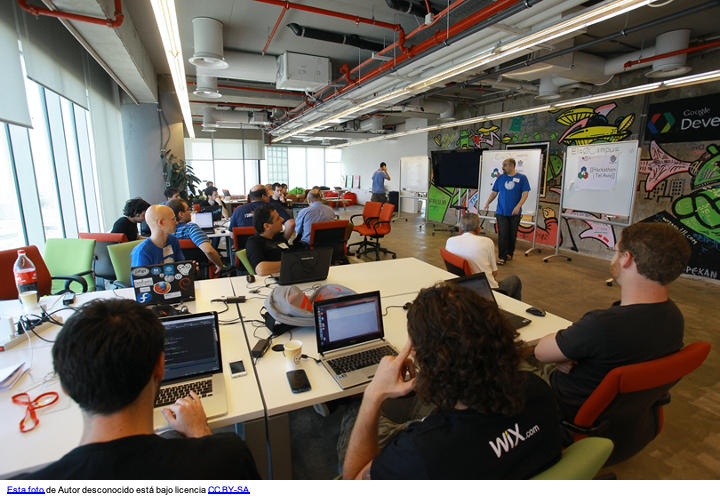
\includegraphics[scale=1.6]{Pictures/hackpng.png}}} % Image background
%\AddToShipoutPicture*{\put(0,0){\includegraphics[height=900, width=650]{Pictures/exponential.png}}} % Image background
\centering
\vspace*{11.3cm}
\par\normalfont\fontsize{35}{35}\sffamily\selectfont

\begin{center}
    % List of Latex Colour names here: https://www.overleaf.com/learn/latex/Using_colours_in_LaTeX
    \textbf{\color{Orange} \mytitle}  % Modify the name of the colour used to suit your image
    
    %\textbf{\color{White}(\ILMCode)} % Modify the name of the colour used to suit your image
    
    %\color{black}ILM\par % Modify the name of the colour used to suit your image
  \end{center}

   \vspace*{5cm}
   \LARGE  \color{white} \textbf{\author \\} % Modify the name of the colour used to suit your image

    %(\id)\par  


\endgroup

%----------------------------------------------------------------------------------------
%	COPYRIGHT PAGE
%----------------------------------------------------------------------------------------


\newpage
~\vfill
\thispagestyle{empty}

%\noindent \textbf{Statement of confirmation of authenticity}
%\vspace{0.5cm}

%\noindent By the act of making this submission, the learner declares that this is the work of the learner named on the cover sheet. The work has not, in whole or in part, been knowingly presented elsewhere for assessment, or where assessment has been built on a previous assessment, this has been identified. Where materials have been used from other sources it has been properly acknowledged. If this statement is untrue, the learner acknowledges that an assessment offence has been committed.
%Attention is drawn to the plagiarism and cheating policies of both the centre and of ILM. Plagiarism can result in a learner being withdrawn from a qualification.
%\vspace{1cm}

\noindent \textbf{Objetivo de este documento}
\vspace{0.5cm}

\noindent Este documento ha sido preparado para introducir los temas a tratar durante el curso: Seguridad TI. Favor no compartir este documento con terceros que no sean miembros actuales de este curso (de este semestre - segundo semestre 2025) dado que es un documento de uso interno aún en preparación. Si usted por error tiene este documento, por favor elimínelo.


%\begin{wrapfigure}{r}{60mm}
 % \begin{center}
  %  
\includegraphics[scale=0.5]{RT.jpg}
  %\end{center}
%\end{wrapfigure}
% \noindent \textbf{ROMINA TORRES} recibió en 2014 su grado de Doctor en Ingeniería Informática de la Universidad Técnica Federico Santa María. Egresada de Ingeniería Civil Informática realizó pasantías en las empresas KLA-Tencor y Synopsys el año 2001 y 2002 respectivamente en Silicon Valley, Estados Unidos. Posterior. a ello, trabajó para Motorola Software Group Valparaíso y Software AG. El 2012 realizó su pasantía doctoral en el Instituto INRIA, Rocquencourt, París, Francia. Entre el 2013-2020 fue directora de las carreras Informáticas de la Universidad Andrés Bello de la sede Viña del Mar. Entre el 2020 e inicios del 2023 fue Directora del Magister en Ciencias de la Computación y del Magister en Gestión de TI y Telecomunicaciones en la misma casa de estudios. Recibió el premio de mujer destacada Viña del Mar 2020 en la categoría innovación. Entre el 2019 y 2021 fue la directora alterna del FONDEF IDEA Ciencia ``Sistema Inteligente para la telerehabilitación cardiovascular. 
 %Desde el 2018 colabora con el Instituto Nacional de Ciberseguridad en formación para hacer de Valparaíso la capital de ciberseguridad del pacífico sur. Es la Investigadora Responsable de un Fondecyt de Iniciación 2022-2024: ``Framework for detecting, monitoring and analyzing multi-stage attacks in evolution during runtime''. Desde Abril 2023 es académica de la Facultad de Ingeniería y Ciencias de la Universidad Adolfo Ibáñez.  \textbf{e-mail:} romina.torres.t@uai.cl. \textbf{twitter:} @rominabot. %\textbf{Sitio Web:} \url{http://www.informatica-unab-vm.cl/profesores/romina.torres/}.  



\vspace{1cm}

%\noindent \textsc{\ILMCentreName - Report for the Award of a Level \ILMLevel Certificate from the Institute of Leadership and Management}\\

%\noindent This was written by \author, to be approved for submission by \reviewer. Written at the \ILMCentreName  (\ILMCentreCode).\\ % License information

\noindent \textit{ Liberación v0.2, \date. romibot} % Printing/edition date

%----------------------------------------------------------------------------------------
%	TABLE OF CONTENTS
%----------------------------------------------------------------------------------------

\chapterimage{diferente2.png} % Table of contents heading image
\vspace{20px}
\pagestyle{empty} % No headers

\tableofcontents % Print the table of contents itself

%\listoftables %uncomment this if you want to print the list of tables at the start

\pagestyle{fancy} % Print headers again


%----------------------------------------------------------------------------------------
%	Glossary
%----------------------------------------------------------------------------------------

\chapterimage{ampolletas.png} % Table of contents heading image
\vspace{20px}

\chapterimage{Pictures/networks.jpg}
\chapter{Repaso: Fundamentos de Redes para Seguridad de TI}
\vspace{65px}
\begin{flushright}
    \textit{Las redes son la columna vertebral de la comunicación digital moderna.}
\end{flushright}



Una red de computadoras es un grupo de computadoras y dispositivos conectados entre sí para compartir datos, información o recursos. 
Las redes y las telecomunicaciones son fundamentales para permitir la interacción y transacciones. Los componentes de hardware (HW) y software (SW) proveen estas funciones de comunicación y son críticas para la infraestructura del negocio, sumándose actualmente kits de servicios basados en nube. 

En 1966 existe la primera red que conectó dos computadores. El Gobierno de Estados Unidos inicia el proyecto ARPANET. Fue en octubre de 1969 cuando se envió el primer mensaje host-to-host desde el laboratorio de Kleinrock en la UCLA para SRI. Pronto otros dos nodos fueron agregados en la UC Santa Barbara y la Universidad de Utah. Al final de ese año las cuatro computadoras estaban conectadas en ARPANET, y con ello nacía la internet. 

\section{Modelo de capas y arquitectura de red}

\subsection{El problema de la complejidad}

Las redes enfrentan varios desafíos fundamentales de complejidad que requieren enfoques sistemáticos para su resolución. El número extremadamente grande de computadoras conectadas, que asciende a miles de millones de dispositivos en todo el mundo, presenta un desafío logístico y técnico sin precedentes. Esta escala masiva requiere arquitecturas que puedan manejar eficientemente la comunicación entre un número prácticamente ilimitado de dispositivos.

La variedad increíble de tecnologías utilizadas en las redes modernas añade otra capa de complejidad significativa. Cada tecnología presenta diferentes restricciones técnicas, limitaciones de ancho de banda, y características de latencia que deben ser consideradas en el diseño de protocolos de comunicación. Esta diversidad tecnológica incluye desde conexiones de fibra óptica de alta velocidad hasta comunicaciones satelitales con latencia elevada.

La ausencia de una entidad administrativa única en Internet representa un desafío fundamental, ya que Internet es esencialmente una red de redes donde cada organización mantiene control sobre su propia infraestructura. Esta descentralización requiere protocolos y estándares que permitan la interoperabilidad sin necesidad de coordinación centralizada. Finalmente, las demandas y aplicaciones en evolución constante presentan nuevos requisitos de rendimiento, seguridad y funcionalidad que deben ser atendidos por la infraestructura de red existente.

\subsection{Solución: Capas de abstracción}

Para manejar la complejidad inherente de las redes modernas, se utiliza el concepto fundamental de capas de abstracción, que proporciona una metodología sistemática para dividir y conquistar problemas complejos. La separación de preocupaciones es el principio rector que permite dividir el problema de comunicación de red en partes separadas y manejables, donde cada componente se enfoca en una función específica sin preocuparse por los detalles de implementación de otras partes.

La solución independiente de cada capa permite que los desarrolladores y ingenieros resuelvan cada parte por separado, optimizando cada componente según sus requisitos específicos sin afectar la funcionalidad de otras capas. Las interfaces comunes establecen contratos bien definidos entre capas, permitiendo que diferentes implementaciones coexistan siempre que respeten estos acuerdos de interfaz. Este enfoque facilita la interoperabilidad entre sistemas de diferentes fabricantes y tecnologías.

La encapsulación es un concepto crucial donde los datos de una capa se encapsulan dentro de la capa inferior, creando una estructura jerárquica donde cada nivel añade su propia información de control sin exponer los detalles internos a las capas superiores. Finalmente, la evolución independiente permite que cada capa evolucione por separado, facilitando la innovación tecnológica sin requerir cambios en toda la pila de protocolos.

\textbf{Regla importante}: "Sé estricto en lo que envías y verifica cuidadosamente lo que recibes"

\subsection{Modelo de referencia OSI}

El modelo OSI (Open Systems Interconnection) define siete capas de abstracción:

\begin{enumerate}
    \item \textbf{Capa 7 - Aplicación}: Interfaz con aplicaciones de usuario
    \item \textbf{Capa 6 - Presentación}: Codificación, compresión y encriptación
    \item \textbf{Capa 5 - Sesión}: Gestión de sesiones de comunicación
    \item \textbf{Capa 4 - Transporte}: Comunicación confiable entre procesos
    \item \textbf{Capa 3 - Red}: Enrutamiento entre redes
    \item \textbf{Capa 2 - Enlace de datos}: Transmisión en red local
    \item \textbf{Capa 1 - Física}: Transmisión de bits por medio físico
\end{enumerate}

\subsection{Modelo TCP/IP}

El modelo TCP/IP es más simple y práctico, con cuatro capas:

\begin{enumerate}
    \item \textbf{Capa de Aplicación}: Combina las capas 5, 6 y 7 del OSI
    \item \textbf{Capa de Transporte}: Corresponde a la capa 4 del OSI
    \item \textbf{Capa de Internet}: Corresponde a la capa 3 del OSI
    \item \textbf{Capa de Acceso a Red}: Combina las capas 1 y 2 del OSI
\end{enumerate}

\subsection{Capas 1 y 2: Física y Enlace de Datos}

\subsubsection{Capa 1: Capa Física}

La capa física representa la base fundamental de toda comunicación de red, siendo responsable de la codificación de bits para enviar por un enlace físico único. Esta capa define las características específicas del hardware y medio de transmisión, estableciendo los estándares que gobiernan cómo los datos se convierten en señales físicas que pueden viajar a través de diferentes medios.

Los ejemplos más comunes incluyen Ethernet para redes cableadas, que especifica cómo enviar bits a través de cables de cobre, y el estándar 802.11 WiFi para comunicaciones inalámbricas, que define cómo los datos se transmiten como ondas de radio. Esta capa es crucial porque determina las limitaciones fundamentales de velocidad, distancia y confiabilidad de la comunicación, estableciendo los parámetros básicos que todas las capas superiores deben respetar.

\subsubsection{Capa 2: Capa de Enlace}

La capa de enlace maneja el encapsulado y transmisión de bits en mensajes individuales enviados a través de una subred única, proporcionando el mecanismo para que los dispositivos en la misma red local se comuniquen de manera efectiva. Esta capa es responsable del direccionamiento local mediante direcciones MAC, que identifican únicamente cada dispositivo en la red local.

Una característica importante de esta capa es que a menudo la tecnología soporta broadcast, permitiendo que un mensaje sea enviado a todos los dispositivos en la red simultáneamente. Los ejemplos incluyen Ethernet para redes cableadas y 802.11 WiFi para redes inalámbricas, ambos especificando cómo enviar paquetes a un host específico en esta red. Esta capa también maneja la detección y corrección de errores a nivel de enlace, asegurando que los datos lleguen intactos al siguiente salto en la red.

\subsubsection{Direcciones MAC}

Las direcciones MAC (Media Access Control) representan identificadores únicos de 48 bits asignados a cada interfaz de red, proporcionando un mecanismo fundamental para la identificación de dispositivos en el nivel de enlace de datos. El formato estándar de estas direcciones permite una identificación precisa del fabricante del dispositivo, ya que los primeros 3 bytes, conocidos como OUI (Organizationally Unique Identifier), indican específicamente qué empresa manufacturó la interfaz de red.

Los últimos 3 bytes de la dirección MAC son únicos por fabricante, garantizando que no existan conflictos de direcciones dentro de la infraestructura de red de una empresa específica. La escritura convencional utiliza formato hexadecimal delimitado por dos puntos, como en el ejemplo BC:5F:F4:2B:E9:68, facilitando la lectura y manipulación por parte de administradores de red y herramientas de diagnóstico.

Es importante destacar que el alcance de las direcciones MAC es limitado, siendo significativas únicamente dentro de una red local, ya sea cableada o inalámbrica. Esta limitación de alcance es una característica de diseño que previene conflictos de direcciones en redes globales y simplifica la administración de redes locales.

\subsubsection{Protocolo ARP}

El Protocolo de Resolución de Direcciones (ARP) es fundamental para el funcionamiento de las redes IP, permitiendo encontrar la dirección MAC correspondiente a una dirección IP dada. Este protocolo establece un mapeo dinámico entre direcciones IP y direcciones MAC, resolviendo la diferencia fundamental entre el direccionamiento lógico de la capa de red y el direccionamiento físico de la capa de enlace.

El proceso de resolución ARP funciona mediante consultas a dispositivos en la red local, donde un dispositivo que necesita comunicarse con una dirección IP específica envía una solicitud broadcast preguntando qué dispositivo posee esa dirección IP. La información obtenida a través de ARP permite identificar no solo la dirección MAC del dispositivo destino, sino también información sobre el fabricante del dispositivo, ya que el OUI de la dirección MAC revela qué empresa manufacturó el hardware.

Por ejemplo, un dispositivo identificado como "TB-Galaxy-S7" puede ser reconocido por su OUI específico, proporcionando información valiosa para la administración de red y la seguridad. Este protocolo es esencial para el funcionamiento de cualquier red IP, ya que sin él, los dispositivos no podrían determinar cómo enviar paquetes a destinos específicos en la red local.

\subsection{Capa 3: Red}

\subsubsection{Protocolo de Internet (IP)}

El Protocolo de Internet (IP) es el componente fundamental que permite conectar múltiples subredes para proporcionar conectividad de extremo a extremo a través de redes heterogéneas. Este protocolo proporciona direccionamiento global mediante direcciones IP únicas, permitiendo que cualquier dispositivo en Internet pueda ser identificado y alcanzado desde cualquier otro punto de la red global.

Una característica importante del protocolo IP es que solo proporciona entrega de mejor esfuerzo, lo que significa que no garantiza la llegada de paquetes ni su orden de llegada. Esta característica de diseño permite que IP funcione de manera eficiente a través de diferentes tecnologías de enlace, desde conexiones de alta velocidad hasta enlaces lentos e inestables, adaptándose a las condiciones cambiantes de la red.

La flexibilidad del protocolo IP para funcionar sobre diferentes tecnologías de enlace es una de sus fortalezas principales, permitiendo que la misma infraestructura de red soporte desde conexiones Ethernet de alta velocidad hasta comunicaciones satelitales con latencia elevada. Esta versatilidad ha sido fundamental para el éxito y la expansión global de Internet.

\subsubsection{Direcciones IPv4}

Las direcciones IPv4 representan el esquema de direccionamiento fundamental de Internet, utilizando un formato de 32 bits que teóricamente proporciona direcciones únicas globalmente. La escritura convencional utiliza formato decimal punteado de cuatro bytes, como en el ejemplo "141.9.68.24", donde cada octeto puede tener valores entre 0 y 255, proporcionando un rango total de direcciones desde 0.0.0.0 hasta 255.255.255.255.

El sistema de direccionamiento IPv4 implementa un esquema de subredes donde los bits se dividen en porciones de red y host, permitiendo una organización jerárquica de las direcciones. La notación CIDR, como 181.41.0.0/18, indica específicamente cuántos bits están reservados para la porción de red, determinando el número de hosts disponibles en esa subred. El cálculo del número de hosts disponibles sigue la fórmula $2^{(32-n)} - 2$, donde n es el número de bits de red y se restan 2 direcciones reservadas para la dirección de red y la dirección de broadcast.

Este esquema de direccionamiento ha sido fundamental para el crecimiento de Internet, aunque la limitación de 32 bits ha llevado al desarrollo de IPv6 para abordar la escasez de direcciones que se ha vuelto crítica con la proliferación de dispositivos conectados.

\subsubsection{Direcciones especiales IPv4}

El esquema de direccionamiento IPv4 incluye varias categorías de direcciones especiales que cumplen funciones específicas en el funcionamiento de las redes. La dirección de loopback, 127.0.0.1, siempre se refiere a la máquina local, permitiendo que las aplicaciones se comuniquen consigo mismas sin necesidad de utilizar la red física. Esta dirección es fundamental para el desarrollo y testing de aplicaciones de red.

Las direcciones privadas, que incluyen los rangos 10.0.0.0/8, 172.16.0.0/12, y 192.168.0.0/16, están reservadas para uso interno en redes privadas y no son enrutadas en Internet público. Estas direcciones permiten que múltiples organizaciones utilicen el mismo espacio de direcciones sin conflictos, facilitando la implementación de redes internas sin consumir direcciones públicas limitadas.

Las direcciones link-local, en el rango 169.254.0.0/16, son auto-asignadas por dispositivos cuando no pueden obtener una dirección IP a través de DHCP, proporcionando conectividad básica en situaciones donde no hay un servidor de configuración disponible. Finalmente, NAT (Network Address Translation) es una técnica fundamental que permite traducir direcciones privadas a direcciones públicas, conservando el limitado espacio de direcciones IPv4 públicas mientras permite que múltiples dispositivos privados accedan a Internet.

\subsubsection{IPv6}

IPv6 representa la nueva iteración del esquema de direccionamiento del Protocolo de Internet, diseñada específicamente para abordar la escasez crítica de direcciones IPv4. Con un tamaño de 128 bits en lugar de los 32 bits de IPv4, IPv6 proporciona un espacio de direcciones prácticamente ilimitado, con capacidad para $2^{128}$ direcciones únicas, resolviendo definitivamente los problemas de agotamiento de direcciones que enfrenta IPv4.

La escritura de direcciones IPv6 utiliza palabras hexadecimales de 16 bits delimitadas por dos puntos, como en el ejemplo 2001:0db8:85a3:0000:0000:8a2e:0370:7334. Este formato más largo permite una representación más clara de la jerarquía de direcciones y facilita la implementación de características avanzadas como autoconfiguración y movilidad.

El despliegue de IPv6 ha estado en progreso durante los últimos 25 años, con una transición gradual desde IPv4 que ha requerido la implementación de tecnologías de transición como túneles y traducción de direcciones. A pesar de los desafíos de migración, IPv6 es esencial para el futuro crecimiento de Internet y la proliferación de dispositivos IoT, proporcionando la base para una conectividad verdaderamente global y escalable.

\subsection{Capa 4: Transporte}

\subsubsection{Tipos de servicios}

La capa de transporte proporciona dos tipos principales de servicios que satisfacen diferentes necesidades de las aplicaciones. UDP (User Datagram Protocol) ofrece datagramas no confiables, priorizando la velocidad y eficiencia sobre la garantía de entrega, siendo ideal para aplicaciones donde la pérdida ocasional de datos es aceptable, como streaming de video o juegos en línea.

TCP (Transmission Control Protocol) proporciona un flujo de bytes confiable, garantizando que todos los datos lleguen al destino en el orden correcto y sin errores. Este protocolo mantiene un registro detallado de los datos recibidos y retransmite automáticamente cualquier segmento que se pierda o llegue corrupto, siendo esencial para aplicaciones donde la integridad de los datos es crítica, como transferencia de archivos, correo electrónico y navegación web.

La confiabilidad en TCP se logra mediante mecanismos sofisticados de control de flujo, control de congestión y recuperación de errores, que trabajan en conjunto para asegurar una comunicación robusta incluso en condiciones de red adversas.

\subsubsection{Comunicación sin conexión vs. orientada a conexión}

La comunicación sin conexión, implementada por UDP, es similar a IP plano, proporcionando poco servicio adicional más allá del direccionamiento básico. En este modo, cada paquete se envía independientemente sin establecer una conexión previa, siendo ideal para aplicaciones donde la simplicidad y la velocidad son más importantes que la confiabilidad.

La comunicación orientada a conexión, implementada por TCP, proporciona comunicación confiable y sin errores mediante el establecimiento de una conexión virtual entre el origen y el destino antes de transmitir datos. Este enfoque incluye mecanismos de control de flujo, control de congestión y recuperación de errores, asegurando que los datos lleguen completos y en el orden correcto.

\subsubsection{Protocolo UDP}

El Protocolo de Datagramas de Usuario (UDP) permite a las aplicaciones enviar datagramas IP de manera simple y eficiente, proporcionando un servicio mínimo de transporte que prioriza la velocidad sobre la confiabilidad. La encapsulación en UDP es extremadamente ligera, con solo 8 bytes de encabezado seguidos directamente por la carga útil de datos, minimizando la sobrecarga de procesamiento y permitiendo transmisiones rápidas.

Las características distintivas de UDP incluyen la ausencia de control de flujo, lo que significa que no regula la velocidad de transmisión para evitar saturar al receptor, y la falta de control de errores, ya que no detecta ni corrige errores de transmisión automáticamente. Además, UDP no implementa retransmisión de paquetes perdidos, confiando en que las aplicaciones de nivel superior manejen estos aspectos si son necesarios.

UDP encuentra su aplicación ideal en situaciones cliente-servidor simples donde la simplicidad y la velocidad son más importantes que la confiabilidad, como en consultas DNS, donde una respuesta rápida es más valiosa que garantizar que cada consulta llegue perfectamente. Este protocolo también es fundamental para aplicaciones de tiempo real donde la latencia baja es crítica y la pérdida ocasional de datos es aceptable.

\subsubsection{Puertos}

Los puertos representan un mecanismo fundamental de multiplexación a nivel de aplicación, permitiendo que múltiples servicios y aplicaciones coexistan en un mismo dispositivo sin conflictos. Cada proceso que necesita utilizar servicios de red se adjunta a un puerto específico mediante la operación BIND, estableciendo un punto de entrada único para las comunicaciones destinadas a esa aplicación.

Cuando llega un paquete UDP o TCP, el puerto destino determina a qué proceso específico se debe entregar la carga útil del paquete, permitiendo que un solo dispositivo pueda ejecutar simultáneamente un servidor web, un servidor de correo, y otros servicios sin interferencia. El puerto origen es utilizado principalmente cuando se necesita una respuesta, permitiendo que el proceso destino sepa a qué puerto debe enviar su respuesta.

Este sistema de puertos es esencial para el funcionamiento de Internet, ya que permite que miles de aplicaciones diferentes funcionen simultáneamente en millones de dispositivos, cada una identificada únicamente por la combinación de dirección IP y número de puerto. Los puertos están numerados del 0 al 65535, con rangos específicos reservados para diferentes tipos de servicios y aplicaciones.

\subsubsection{Protocolo TCP}

El Protocolo de Control de Transmisión (TCP) está diseñado específicamente para proporcionar flujo de bytes confiable de extremo a extremo sobre redes que pueden ser no confiables, incorporando mecanismos sofisticados para garantizar la integridad y orden de los datos transmitidos. Este protocolo es robusto contra fallas y cambios en las propiedades de red, adaptándose dinámicamente a condiciones cambiantes como congestión, pérdida de paquetes y variaciones en la latencia.

TCP maneja flujos TCP e interfa eficientemente con la capa IP, aceptando flujos de datos de procesos de aplicación y dividiéndolos en piezas no mayores a 64 KB para su transmisión. El tamaño típico de segmento TCP es de 1460 bytes de datos, optimizado para caber eficientemente en un frame Ethernet estándar de 1500 bytes, maximizando la utilización del ancho de banda disponible.

Este protocolo se utiliza para situaciones donde la precisión y completitud de los datos son críticas, como compartir archivos, navegar por Internet o enviar correo electrónico. En estos casos, tener solo una porción parcial de los datos puede hacer que toda la información sea inútil, por lo que TCP garantiza que los datos sean precisos y completos antes de entregarlos a la aplicación.

\subsection{Sistema de nombres de dominio (DNS)}

El Sistema de Nombres de Dominio (DNS) es fundamental para el funcionamiento de Internet, ya que traduce nombres de dominio legibles por humanos en direcciones IP numéricas.

\subsubsection{Jerarquía de servidores DNS}

El DNS utiliza una estructura jerárquica de servidores que permite una distribución eficiente de la responsabilidad de resolución de nombres. Los servidores raíz representan el nivel más alto de esta jerarquía, manteniendo información sobre cómo encontrar servidores autoritativos para todas las zonas de nivel superior como .com, .org, .edu y .gov. Estos servidores son fundamentales para el funcionamiento global de Internet, ya que proporcionan el punto de entrada inicial para cualquier consulta DNS.

Los servidores de nivel superior manejan dominios específicos como .com, .org, .edu, .gov, y otros dominios de país como .cl, .ar, .mx. Estos servidores conocen la ubicación de los servidores autoritativos para cada dominio específico dentro de su zona de responsabilidad. Los servidores autoritativos son responsables de zonas específicas de dominio, manteniendo la información precisa sobre las direcciones IP correspondientes a los nombres de dominio en su zona.

Los servidores locales, también conocidos como resolvers, son los que consultan otros servidores DNS en nombre de las aplicaciones cliente. Estos servidores suelen ser proporcionados por los proveedores de servicios de Internet o configurados localmente en redes corporativas, actuando como intermediarios entre las aplicaciones y la infraestructura DNS global.

\subsubsection{Resolución de nombres}

El proceso de resolución DNS sigue una secuencia específica de pasos diseñada para encontrar eficientemente la dirección IP correspondiente a un nombre de dominio. El proceso comienza cuando un programa solicita la IP de un nombre de dominio, iniciando una cadena de consultas que involucra múltiples servidores DNS en la jerarquía global.

La consulta local es el primer paso, donde el resolver local consulta su servidor DNS configurado, que suele ser proporcionado por el proveedor de servicios de Internet. El servidor verifica si puede responder directamente a la consulta, lo cual es posible si la información está en su caché local o si es autoritativo para ese dominio específico.

Si el servidor local no puede responder directamente, inicia una consulta recursiva que sigue la jerarquía DNS desde la raíz hacia abajo. Esta consulta puede involucrar múltiples servidores DNS, cada uno proporcionando información sobre el siguiente paso en la cadena de resolución. Finalmente, cuando se obtiene la respuesta, se envía de vuelta al resolver original, que la entrega a la aplicación que hizo la consulta inicial.

\subsubsection{Configuración de DNS}

Cada zona DNS requiere una configuración específica que incluye múltiples servidores para garantizar la redundancia y disponibilidad del servicio. El servidor primario mantiene el archivo de zona con toda la información autoritativa sobre los nombres de dominio en esa zona específica. Este servidor es responsable de las actualizaciones y modificaciones en la información de la zona, siendo el punto de autoridad definitivo para esa porción del espacio de nombres DNS.

El servidor secundario proporciona redundancia crítica al copiar los datos del servidor primario, asegurando que el servicio DNS continúe funcionando incluso si el servidor primario falla. Esta configuración de respaldo es esencial para la confiabilidad del sistema DNS, ya que permite que las consultas se resuelvan desde múltiples ubicaciones geográficas y administrativas.

Las actualizaciones en la información DNS se realizan siempre en el servidor primario, que luego replica automáticamente estos cambios al servidor secundario mediante un proceso de transferencia de zona. Este mecanismo de replicación asegura que todos los servidores DNS para una zona específica mantengan información consistente y actualizada.

\subsubsection{Seguridad DNS}

El DNS presenta varias vulnerabilidades de seguridad críticas que pueden comprometer la integridad y confidencialidad de las comunicaciones de red. El DNS spoofing es una técnica donde los atacantes falsifican respuestas DNS, redirigiendo a los usuarios a sitios web maliciosos que imitan sitios legítimos. Esta técnica es particularmente peligrosa porque puede permitir el robo de credenciales y datos sensibles sin que el usuario se dé cuenta de que está en un sitio falso.

El DNS cache poisoning es otra amenaza significativa donde los atacantes contaminan la caché DNS de servidores legítimos, causando que múltiples usuarios sean redirigidos a sitios maliciosos durante períodos prolongados. El DNS tunneling es una técnica más sofisticada donde los atacantes utilizan el protocolo DNS para evadir firewalls y otros controles de seguridad, transmitiendo datos maliciosos a través de consultas DNS aparentemente legítimas.

Los ataques DNS amplification representan una amenaza de denegación de servicio, donde los atacantes utilizan servidores DNS públicos para amplificar el tráfico malicioso, causando interrupciones significativas en servicios críticos. Estos ataques pueden ser especialmente devastadores porque pueden generar volúmenes de tráfico extremadamente altos con relativamente poco esfuerzo del atacante.

\subsubsection{Medidas de protección DNS}

Para proteger contra los ataques DNS, se han desarrollado varias medidas de seguridad que abordan las vulnerabilidades específicas del protocolo. DNSSEC (DNS Security Extensions) es una extensión fundamental que proporciona autenticación y verificación de integridad para las respuestas DNS, utilizando criptografía de clave pública para asegurar que las respuestas provengan de servidores autorizados y no hayan sido modificadas en tránsito.

DNS over HTTPS (DoH) y DNS over TLS (DoT) son tecnologías que encriptan las consultas DNS, previniendo que los atacantes intercepten y manipulen las comunicaciones DNS. Estas tecnologías son especialmente importantes en redes públicas donde las consultas DNS pueden ser interceptadas fácilmente. El filtrado de DNS es otra medida importante que bloquea dominios maliciosos conocidos, previniendo que los usuarios accedan a sitios web peligrosos.

Estas medidas de protección trabajan en conjunto para crear múltiples capas de seguridad que hacen más difícil para los atacantes comprometer el sistema DNS. La implementación de estas medidas es esencial para mantener la confiabilidad y seguridad de las comunicaciones de red modernas.

\begin{itemize}
    \item \textbf{Dirección MAC}: Identificador único del hardware
    \item \textbf{Dirección IPv6}: Link local - no enrutada a internet
    \item \textbf{Dirección IPv4}: IP privada enrutada por NAT
    \item \textbf{Máscara de subred}: Muestra que es una red /24
    \item \textbf{Información DHCP}: Información de arrendamiento
    \item \textbf{Puerta de enlace}: IP a la que enviamos para llegar a internet
    \item \textbf{Servidor DNS}: IP para buscar nombres
\end{itemize}

\subsubsection{Configuración Linux}

\begin{itemize}
    \item \textbf{Dirección MAC}: Identificador único del hardware
    \item \textbf{Máscara de subred}: Muestra que es una red /24
    \item \textbf{Dirección IPv4}: IP privada enrutada por NAT
    \item \textbf{Dirección IPv6}: Link local - no enrutada a internet
    \item \textbf{Servidor DNS}: IP para buscar nombres
    \item \textbf{Puerta de enlace}: IP a la que enviamos para llegar a internet
\end{itemize}



A medida que se conectan más y más dispositivos, se vuelve cada vez más difícil obtener una dirección pública que no esté ya en uso. Por ejemplo, Cisco, un gigante de la industria en el mundo de las redes, estimó que habría aproximadamente 50 mil millones de dispositivos conectados a Internet para fines de 2021. (Cisco., 2021) . Utilizando el esquema de direccionamiento del Protocolo de Internet conocido como IPv4, que utiliza un sistema de numeración de 2\^32 direcciones IP se tienen 4,29 mil millones de puntos. 
IPv6 es una nueva iteración del esquema de direccionamiento del Protocolo de Internet para ayudar a abordar este problema. 
Admite hasta 2\^128 de direcciones IP (más de 340 billones), resolviendo los problemas que enfrenta IPv4. Ejemplo:\\
 IPv4 $192.168.10.150 $ vs  \\IPv6 $3002:0bd6:0000:0000:0000:ee00:0033:6778$


La división en subredes se logra dividiendo la cantidad de hosts que pueden caber dentro de la red, representados por un número llamado máscara de subred.  una máscara de subred que también se representa como un número de cuatro bytes (32 bits), que van de 0 a 255 (0-255). Las subredes usan direcciones IP de tres maneras diferentes:
\begin{itemize}
    \item Identificar la dirección de red: identifica el inicio de la red real y se utiliza para identificar la existencia de una red. Por ejemplo, un dispositivo con la dirección IP 192.168.1.100 estará en la red identificada por 192.168.1.0 
\item Identificar la dirección del host: se usa para identificar un dispositivo en la subred. 
\item Identificar la puerta de enlace predeterminada: dirección especial asignada a un dispositivo en la red que es capaz de enviar información a otra red. Estos dispositivos pueden usar cualquier dirección de host, pero generalmente usan la primera o la última dirección de host en una red (.1 o .254). 

\end{itemize}


\textbf{El protocolo ARP o protocolo de resolución de direcciones} para abreviar, es la tecnología que se encarga de permitir que los dispositivos se identifiquen en una red. Permite que un dispositivo asocie su dirección MAC con una dirección IP en la red. Cada dispositivo en una red mantendrá un registro de las direcciones MAC asociadas con otros dispositivos.
Cuando los dispositivos deseen comunicarse con otros, enviarán una transmisión a toda la red en busca del dispositivo específico. Los dispositivos pueden usar el protocolo ARP para encontrar la dirección MAC (y por lo tanto el identificador físico) de un dispositivo para la comunicación.

Cada dispositivo dentro de una red tiene un registro para almacenar información, que se denomina caché. En el contexto del  protocolo ARP  , este caché almacena los identificadores de otros dispositivos en la red.
%
Para mapear estos dos identificadores juntos (dirección IP y dirección MAC ), el protocolo ARP envía dos tipos de mensajes:
Solicitud ARP y 
Respuesta ARP. \\
Cuando se envía una solicitud ARP , se transmite un mensaje a todos los demás dispositivos encontrados en una red por el dispositivo, preguntando si la dirección MAC del dispositivo coincide o no con la dirección IP solicitada. Si el dispositivo tiene la dirección IP solicitada, se devuelve una respuesta ARP al dispositivo inicial para confirmarlo. El dispositivo inicial ahora recordará esto y lo almacenará dentro de su caché (una entrada ARP ). 

Las direcciones IP se pueden asignar de forma manual, introduciéndolas físicamente en un dispositivo, o de forma automática y más comúnmente mediante el uso de un servidor DHCP ( D ynamic H ost C onfiguration P rotocol). Cuando un dispositivo se conecta a una red, si aún no se le ha asignado manualmente una dirección IP, envía una solicitud ( DHCP Discover) para ver si hay algún servidor DHCP en la red. Luego, el servidor DHCP responde con una dirección IP que el dispositivo podría usar (oferta de DHCP). Luego, el dispositivo envía una respuesta confirmando que desea la dirección IP ofrecida (solicitud DHCP) y, por último, el servidor DHCP envía una respuesta reconociendo que esto se ha completado y que el dispositivo puede comenzar a usar la dirección IP (DHCP ACK).




Hay múltiples métodos para conectarse a Internet. ISP  - usando fibra óptica lo que permite conexiones más rápidas que otras opciones. Depende de donde la persona vive. Existe mediante satélite y a la antigua con servicios de dialup, o inalámbricamente. 

Smartphones se conectan a redes móviles de múltiples generaciones, evolucionando desde la 3ra generación hasta la actual 5ta generación, con desarrollo activo de la 6ta generación. Ellos se conectan a redes Wi-Fi usando estándar 802.11. 

\subsubsection{Evolución de las redes móviles}

\begin{itemize}
    \item \textbf{3G (Tercera Generación)}: Introdujo Internet móvil de alta velocidad, videollamadas y navegación web móvil. Velocidades típicas: 384 Kbps - 2 Mbps.
    
    \item \textbf{4G/LTE (Cuarta Generación)}: Revolucionó la conectividad móvil con velocidades de hasta 100 Mbps, streaming de video HD, y aplicaciones móviles avanzadas. Tecnología Long Term Evolution (LTE) como estándar principal.
    
    \item \textbf{5G (Quinta Generación)}: Tecnología actual que ofrece velocidades de hasta 10 Gbps, latencia ultra-baja (1ms), y soporte para IoT masivo. Habilita aplicaciones como vehículos autónomos, cirugía remota, y realidad aumentada.
    
    \item \textbf{6G (Sexta Generación)}: En desarrollo activo, se espera que esté disponible comercialmente hacia 2030. Promete velocidades de hasta 1 Tbps, latencia de microsegundos, y soporte para tecnologías emergentes como hologramas, telepresencia inmersiva, y computación cuántica distribuida.
\end{itemize}

Redes Celulares 3G/4G/5G proveen Internet y comunicación por voz estable en un área amplia. Con servicio celular, la conexión a Internet parece continua al usuario, incluso si los dispositivos se mueven de celda a celda. Sin embargo, muchos proveedores imponen límite de transferencia y cargos por acceso o definitivamente bajan la velocidad de conexión cuando los usuarios exceden el límite.

\subsubsection{Características de la 6G}

La sexta generación de redes móviles se enfoca en:

\begin{itemize}
    \item \textbf{Velocidades extremas}: Hasta 1 Tbps (1000 Gbps), 100 veces más rápido que 5G
    \item \textbf{Latencia ultra-baja}: Menos de 1 microsegundo para aplicaciones críticas
    \item \textbf{Conectividad masiva}: Soporte para 10 millones de dispositivos por km²
    \item \textbf{Inteligencia artificial integrada}: Redes autónomas que se optimizan automáticamente
    \item \textbf{Sostenibilidad}: Eficiencia energética extrema y reducción de huella de carbono
    \item \textbf{Seguridad cuántica}: Encriptación resistente a computación cuántica
\end{itemize}

\subsubsection{Aplicaciones futuras de la 6G}

\begin{itemize}
    \item \textbf{Telepresencia holográfica}: Comunicación tridimensional en tiempo real
    \item \textbf{Internet táctil}: Transmisión de sensaciones físicas a través de la red
    \item \textbf{Computación cuántica distribuida}: Redes que conectan computadores cuánticos
    \item \textbf{Realidad extendida}: Fusión perfecta entre mundo físico y digital
    \item \textbf{Medicina remota avanzada}: Cirugía robótica con latencia imperceptible
    \item \textbf{Transporte inteligente}: Sistemas de tráfico autónomos y coordinados
\end{itemize}
Dispositivos celulares pueden actuar como puntos de acceso a otros dispositivos. Estos se conectan a la Internet usando una conexión celular y la convierten a una conexión Wi-Fi para que otros dispositivos se puedan conectar mientras el carrier tenga cobertura. 

\subsubsection{Seguridad en redes móviles vs WiFi}

Aunque 3G, 4G o 5G sean más lentas que una Wi-Fi - son mucho más seguras debido a:

\begin{itemize}
    \item \textbf{Encriptación robusta}: Las redes móviles utilizan algoritmos de encriptación avanzados (AES-256, ChaCha20-Poly1305)
    \item \textbf{Autenticación de red}: Verificación de identidad del operador móvil antes de permitir conexión
    \item \textbf{Aislamiento de tráfico}: Cada usuario tiene su propio canal de comunicación
    \item \textbf{Monitoreo continuo}: Los operadores móviles monitorean constantemente el tráfico en busca de anomalías
    \item \textbf{Actualizaciones de seguridad}: Mejoras continuas en protocolos de seguridad
\end{itemize}

\subsubsection{Vulnerabilidades en redes WiFi}

Las redes WiFi presentan mayores riesgos de seguridad:

\begin{itemize}
    \item \textbf{Evil Twin}: Atacantes crean redes WiFi falsas con nombres similares a redes legítimas
    \item \textbf{Man-in-the-Middle}: Interceptación de tráfico entre el dispositivo y el punto de acceso
    \item \textbf{Wardriving}: Búsqueda de redes WiFi vulnerables para explotación
    \item \textbf{Deauthentication}: Ataques que desconectan dispositivos de la red
    \item \textbf{KRACK}: Vulnerabilidades en el protocolo WPA2
\end{itemize}

\subsubsection{Medidas de seguridad para WiFi}

Para mitigar los riesgos en redes WiFi:

\begin{itemize}
    \item \textbf{Encriptación WPA3}: Último estándar de seguridad WiFi
    \item \textbf{Redes privadas virtuales (VPN)}: Encriptación adicional del tráfico
    \item \textbf{Autenticación 802.1X}: Verificación de identidad antes de permitir acceso
    \item \textbf{Segmentación de red}: Separación de dispositivos IoT y críticos
    \item \textbf{Monitoreo de tráfico}: Detección de dispositivos no autorizados
    \item \textbf{Actualizaciones regulares}: Parches de seguridad para routers y dispositivos
\end{itemize} 


\subsection{Tipos y Topologías de redes}

Redes pueden ser públicas o privadas. 

Las redes WANs conectan sistemas sobre áreas grandes geográficamente. Usualmente conecta redes independientes que permite a las personas comunicarse fácilmente entre otros. La Internet oculta los detalles de este proceso del usuario final. Si se envía un correo el usuario no debe preocuparse de cómo se mueve los datos. El Ingeniero en Seguridad si. En este caso encriptación o utilizar redes privadas. 

A pesar que al final del siglo 20 muchos tipos de redes LAN existían, hoy la mayoría ha convergido a una única tecnología llamada Ethernet. Todos los computadores conectados a un "cable" debían pelear entre ellas para turnarse el uso de la red, lo cual era ineficiente. Afortunadamente, tecnología evolucionó, de manera que cada red tiene un cable dedicado, que conecta cada uno a un switch que controla una porción de la red. 


Una VLAN es una LAN virtual que es creada en el router y switch es una colección de dispositivos de red relacionados logicamente que son vistos como un segmento de una red. Da a administradores la capacidad de separar los segmentos de red sin tener que separar físicamente la red cableando y pueden tambien aislar grupos lógicos de dispositivos para reducir el tráfico de red y aumentar la seguridad.  \textbf{Ejemplo:} una VLAN para HR - toda la información sensible que ciaje en esa red de un computador a otro, queda oculta de computadores no HR. 

\subsection{Topologías}
\begin{itemize}
    \item \textbf{Topología de estrellas:} dispositivos se conectan individualmente a través de un dispositivo de red central, como un conmutador o concentrador. Esta topología es la más común hoy en día debido a su confiabilidad y escalabilidad (vs mantenimiento), a pesar del costo ( más cableado y la compra de equipos de red dedicados). Single point of failure (aunque actualmente son bastante robustos). 
    \item \textbf{Topología de bus: } los datos destinados a cada dispositivo viajan a lo largo del mismo cable, es muy probable que se vuelvan lentos y se produzcan cuellos de botella si los dispositivos dentro de la topología solicitan datos simultáneamente. difícil identificar qué dispositivo está experimentando problemas con los datos que viajan por la misma ruta. Mejor costo. poca redundancia en caso de fallas. 
    \item \textbf{Topología de anillo: } computadores se conectan entre si.  funciona mediante el envío de datos a través del bucle hasta que llega al dispositivo de destino, utilizando otros dispositivos a lo largo del bucle para reenviar los datos. Un dispositivo solo enviará datos recibidos de otro dispositivo en esta topología si no tiene ninguno para enviarse a sí mismo. Si el dispositivo tiene datos para enviar, primero enviará sus propios datos antes de enviar datos desde otro dispositivo. aunque  menos propensas a los cuellos de botella, como dentro de una topología de bus - no es una forma eficiente de que los datos viajen a través de una red
\end{itemize}


\section{Protocolos de Red}

\subsection{Conceptos fundamentales}

\textbf{Protocolo}: conjunto de reglas que gobiernan el formato de mensajes que los computadores intercambian. Gobierna como el equipamiento de red interactúa para entregar la data cruzando la red.

Esto es necesario porque los computadores necesitan un lenguaje común para comunicarse. Hoy la mayoría habla al menos un estándar: 
TCP – Protocolo de control de transmisión, y  
IP – Protocolo de Internet. 

\textbf{TCP/IP} es una suite de protocolos que operan en las capas de red y transporte del modelo de referencia OSI y gobiernan todas las actividades sobre la Internet y la mayoría de las redes de casa y corporaciones. Desarrollado por el departamento de Defensa de Estados Unidos para proveer una infraestructura de red altamente confiable y tolerante a fallos.

\subsection{Arquitectura TCP/IP}

La suite TCP/IP se organiza en cuatro capas principales que corresponden al modelo OSI:

\begin{itemize}
    \item \textbf{Capa de Aplicación}: Corresponde a las capas 5, 6 y 7 del modelo OSI
    \item \textbf{Capa de Transporte}: Corresponde a la capa 4 del modelo OSI
    \item \textbf{Capa de Internet}: Corresponde a la capa 3 del modelo OSI
    \item \textbf{Capa de Acceso a Red}: Corresponde a las capas 1 y 2 del modelo OSI
\end{itemize}

\subsection{Protocolos de la capa de aplicación}

\begin{itemize}
    \item \textbf{HTTP (Puerto 80)}: Protocolo de transferencia de hipertexto para la World Wide Web
    \item \textbf{HTTPS (Puerto 443)}: Versión segura de HTTP con encriptación SSL/TLS
    \item \textbf{FTP (Puerto 21)}: Protocolo de transferencia de archivos
    \item \textbf{SFTP (Puerto 22)}: FTP seguro sobre SSH
    \item \textbf{SMTP (Puerto 25)}: Protocolo de envío de correo electrónico
    \item \textbf{POP3 (Puerto 110)}: Protocolo de recepción de correo electrónico
    \item \textbf{IMAP (Puerto 143)}: Protocolo de acceso a correo electrónico
    \item \textbf{DNS (Puerto 53)}: Sistema de nombres de dominio
    \item \textbf{DHCP (Puertos 67/68)}: Protocolo de configuración dinámica de hosts
    \item \textbf{SNMP (Puerto 161)}: Protocolo simple de administración de red
    \item \textbf{Telnet (Puerto 23)}: Protocolo de terminal virtual (inseguro)
    \item \textbf{SSH (Puerto 22)}: Shell seguro para acceso remoto
\end{itemize}

\subsection{Protocolos de la capa de transporte}

\begin{itemize}
    \item \textbf{TCP (Protocolo de Control de Transmisión)}: Protocolo orientado a conexión que garantiza la entrega confiable de datos
    \item \textbf{UDP (Protocolo de Datagramas de Usuario)}: Protocolo no orientado a conexión que prioriza la velocidad sobre la confiabilidad
    \item \textbf{SCTP (Protocolo de Control de Transmisión de Stream)}: Protocolo híbrido que combina características de TCP y UDP
    \item \textbf{DCCP (Protocolo de Control de Congestión de Datagramas)}: Protocolo para aplicaciones multimedia en tiempo real
\end{itemize}

\subsection{Protocolos de la capa de Internet}

\begin{itemize}
    \item \textbf{IP (Protocolo de Internet)}: Protocolo principal para el direccionamiento y enrutamiento de paquetes
    \item \textbf{ICMP (Protocolo de Mensajes de Control de Internet)}: Protocolo para mensajes de control y diagnóstico
    \item \textbf{IGMP (Protocolo de Gestión de Grupos de Internet)}: Protocolo para gestión de grupos multicast
    \item \textbf{ARP (Protocolo de Resolución de Direcciones)}: Protocolo para mapear direcciones IP a direcciones MAC
    \item \textbf{RARP (Protocolo de Resolución de Direcciones Inverso)}: Protocolo para mapear direcciones MAC a direcciones IP
\end{itemize}

\subsection{Protocolos de la capa de acceso a red}

\begin{itemize}
    \item \textbf{Ethernet (IEEE 802.3)}: Estándar para redes cableadas de área local
    \item \textbf{WiFi (IEEE 802.11)}: Estándar para redes inalámbricas de área local
    \item \textbf{PPP (Protocolo Punto a Punto)}: Protocolo para conexiones punto a punto
    \item \textbf{Frame Relay}: Protocolo para redes de área amplia
    \item \textbf{ATM (Modo de Transferencia Asíncrona)}: Protocolo para redes de alta velocidad
\end{itemize}

\subsection{Protocolo TCP en detalle}

El \textbf{Protocolo de Control de Transmisión} (TCP) está diseñado teniendo en cuenta la confiabilidad y la garantía. Este protocolo reserva una conexión constante entre los dos dispositivos durante el tiempo que se tarda en enviar y recibir los datos. Incorpora la comprobación de errores en su diseño. La verificación de errores es la forma en que TCP puede garantizar que los datos enviados se hayan recibido y vuelto a ensamblar en el mismo orden.

TCP se utiliza para situaciones como compartir archivos, navegar por Internet o enviar un correo electrónico. Este uso se debe a que estos servicios requieren que los datos sean precisos y completos (¡no es bueno tener medio archivo!).

\subsubsection{Características principales de TCP}

\begin{itemize}
    \item \textbf{Orientado a conexión}: Establece una conexión virtual entre el origen y el destino antes de transmitir datos
    \item \textbf{Entrega confiable}: Garantiza que todos los paquetes lleguen al destino en el orden correcto
    \item \textbf{Control de flujo}: Regula la velocidad de transmisión para evitar saturar al receptor
    \item \textbf{Control de congestión}: Adapta la velocidad de transmisión según el estado de la red
    \item \textbf{Recuperación de errores}: Detecta y corrige errores de transmisión automáticamente
\end{itemize}

\subsubsection{Estados de conexión TCP}

Una conexión TCP pasa por varios estados durante su ciclo de vida:

\begin{enumerate}
    \item \textbf{CLOSED}: Estado inicial, no hay conexión
    \item \textbf{LISTEN}: El servidor espera conexiones entrantes
    \item \textbf{SYN\_SENT}: El cliente ha enviado SYN, espera respuesta
    \item \textbf{SYN\_RECEIVED}: El servidor ha recibido SYN, ha enviado SYN+ACK
    \item \textbf{ESTABLISHED}: Conexión establecida, se pueden transmitir datos
    \item \textbf{FIN\_WAIT\_1}: El cliente ha enviado FIN, espera ACK
    \item \textbf{FIN\_WAIT\_2}: El cliente ha recibido ACK de FIN, espera FIN del servidor
    \item \textbf{CLOSE\_WAIT}: El servidor ha recibido FIN, espera que la aplicación cierre
    \item \textbf{LAST\_ACK}: El servidor ha enviado FIN, espera ACK
    \item \textbf{TIME\_WAIT}: El cliente espera un tiempo antes de cerrar completamente
\end{enumerate}




\begin{itemize}
    \item Ventajas de TCP 
    \begin{itemize}
        \item Garantiza la exactitud de los datos.
        \item Capaz de sincronizar dos dispositivos para evitar que el otro se inunde de datos.

\item Realiza muchos más procesos para mayor confiabilidad.

    \end{itemize}
    \item Desventajas de TCP
        \begin{itemize}
            \item Requiere una conexión confiable entre los dos dispositivos. Si no se recibe una pequeña porción de datos, entonces no se puede usar toda la porción de datos.
            \item Una conexión lenta puede provocar un cuello de botella en otro dispositivo, ya que la conexión estará reservada en la computadora receptora todo el tiempo.
%\item 
        \end{itemize}



\end{itemize}



\subsection{Protocolo UDP en detalle}

TCP no es el único protocolo que corre sobre IP. Por ejemplo \textbf{UDP (User Datagram Protocol)} corre en paralelo a TCP en una capa diferente para soportar otros protocolos. Estos dos protocolos comunes proveen diferentes tipos de servicios de transporte útiles para diferentes escenarios. 

UDP no cuenta con las muchas funciones que ofrece TCP, como la verificación de errores y la confiabilidad. De hecho, todos los datos que se envían a través de UDP se envían a la computadora, ya sea que lleguen allí o no. No hay sincronización entre los dos dispositivos ni garantía de entrega.

\subsubsection{Características principales de UDP}

\begin{itemize}
    \item \textbf{No orientado a conexión}: No establece una conexión antes de transmitir datos
    \item \textbf{Entrega no confiable}: No garantiza que los paquetes lleguen al destino
    \item \textbf{Sin control de flujo}: No regula la velocidad de transmisión
    \item \textbf{Sin control de congestión}: No adapta la velocidad según el estado de la red
    \item \textbf{Sin recuperación de errores}: No detecta ni corrige errores automáticamente
    \item \textbf{Transmisión rápida}: Prioriza la velocidad sobre la confiabilidad
\end{itemize}

\subsubsection{Aplicaciones típicas de UDP}

UDP es ideal para aplicaciones donde la velocidad es más importante que la confiabilidad:

\begin{itemize}
    \item \textbf{Streaming de video/audio}: Donde la pérdida ocasional de paquetes es aceptable
    \item \textbf{Juegos en línea}: Donde la latencia baja es crítica
    \item \textbf{DNS}: Consultas rápidas de nombres de dominio
    \item \textbf{DHCP}: Configuración automática de red
    \item \textbf{SNMP}: Monitoreo de red en tiempo real
    \item \textbf{VoIP}: Comunicación de voz sobre IP
\end{itemize}


\begin{itemize}
    \item Ventajas de UDP 
    \begin{itemize}
        \item UDP es mucho más rápido que TCP.
        \item UDP deja la capa de aplicación (software de usuario) para decidir si hay algún control sobre la rapidez con que se envían los paquetes.

    \item UDP no reserva una conexión continua en un dispositivo como lo hace TCP.


    \end{itemize}
    \item Desventajas de UDP
        \begin{itemize}
            \item A UDP no le importa si se reciben los datos.
            \item Es bastante flexible para los desarrolladores de software en este sentido.
            \item Esto significa que las conexiones inestables resultan en una experiencia terrible para el usuario.
        \end{itemize}

UDP es útil en situaciones en las que se envían pequeños fragmentos de datos. Por ejemplo, los protocolos utilizados para descubrir dispositivos ( ARP y DHCP ) o archivos más grandes como transmisión de video (donde está bien si alguna parte del video está pixelada. Los píxeles son solo piezas perdidas de ¡datos!)




\subsection{Paquetes y transmisión de datos}

Los paquetes y los frames son pequeños fragmentos de datos que, cuando se forman juntos, forman un fragmento de información o mensaje más grande.

\subsubsection{Encabezamiento del paquete}

El encabezamiento del paquete está compuesto por:
\begin{itemize}
    \item \textbf{Tiempo para vivir (TTL)}: Este campo establece un temporizador de caducidad para que el paquete no obstruya su red si nunca logra llegar a un host o escapar.
    \item \textbf{Suma de verificación}: Este campo proporciona verificación de integridad para protocolos como TCP/IP. Si se cambia algún dato, este valor será diferente de lo que se esperaba y, por lo tanto, corrupto.
    \item \textbf{Dirección de la fuente}: La dirección IP del dispositivo desde el que se envía el paquete para que los datos sepan a dónde regresar.
    \item \textbf{Dirección de destino}: La dirección IP del dispositivo al que está destinado el paquete para que los datos sepan a dónde viajar a continuación.
\end{itemize}

\subsubsection{¿Cómo viaja la información por la red?}

Cuando una máquina envía datos a otra, el proceso sigue estos pasos:

\begin{enumerate}
    \item \textbf{División en paquetes}: Los datos se dividen en paquetes de tamaño fijo (típicamente 1500 bytes para Ethernet)
    \item \textbf{Encapsulación}: Cada paquete recibe encabezados con información de control
    \item \textbf{Enrutamiento}: Los routers deciden la mejor ruta hacia el destino
    \item \textbf{Transmisión física}: Los paquetes se convierten en señales eléctricas/ópticas
    \item \textbf{Recepción}: La máquina destino recibe y reensambla los paquetes
\end{enumerate}

\subsubsection{¿Por qué puedo ver paquetes que no son para mí?}

En redes conmutadas (switches), cada dispositivo solo recibe paquetes destinados a él. Sin embargo, en ciertas situaciones puedes ver tráfico de otros:

\begin{itemize}
    \item \textbf{Redes con hubs}: Los hubs retransmiten todo el tráfico a todos los puertos
    \item \textbf{Modo promiscuo}: Tu tarjeta de red puede configurarse para capturar todo el tráfico
    \item \textbf{ARP poisoning}: Técnica que redirige tráfico a través de tu máquina
    \item \textbf{Port mirroring}: El switch puede configurarse para duplicar tráfico a un puerto específico
\end{itemize}

\textbf{IMPORTANTE}: En este curso, solo se recomienda analizar tráfico de tu propia máquina por razones de seguridad y ética.

\subsection{¿Cómo funciona la transmisión física de datos?}

\subsubsection{Del software al cable}

Cuando envías un email o visitas una página web, los datos pasan por esta transformación:

\begin{enumerate}
    \item \textbf{Aplicación}: Tu programa (navegador, email) genera los datos
    \item \textbf{Encapsulación TCP/IP}: Los datos se dividen y empaquetan
    \item \textbf{Driver de red}: El sistema operativo prepara los paquetes
    \item \textbf{Tarjeta de red}: Convierte datos digitales en señales físicas
    \item \textbf{Medio físico}: Cable de cobre, fibra óptica o ondas de radio
\end{enumerate}

\subsubsection{Señales en diferentes medios}

\begin{itemize}
    \item \textbf{Cable de cobre (Ethernet)}: Los datos se convierten en impulsos eléctricos que varían entre 0V y 5V
    \item \textbf{Fibra óptica}: Los datos se convierten en pulsos de luz (fotones) que se encienden y apagan
    \item \textbf{WiFi}: Los datos se convierten en ondas de radio que varían en frecuencia y amplitud
\end{itemize}

\subsubsection{¿Por qué 1500 bytes por paquete?}

El tamaño máximo de paquete Ethernet (MTU) está limitado por:

\begin{itemize}
    \item \textbf{Limitaciones físicas}: Capacidad del medio de transmisión
    \item \textbf{Control de errores}: Paquetes más pequeños son más fáciles de retransmitir
    \item \textbf{Latencia}: Paquetes grandes pueden bloquear la red
    \item \textbf{Memoria del hardware}: Los switches y routers tienen buffers limitados
\end{itemize}

\subsubsection{El viaje de un paquete}

Imagina que envías un email a alguien en otro país:

\begin{enumerate}
    \item \textbf{Tu computadora}: Divide el email en paquetes de 1500 bytes
    \item \textbf{Tu router}: Recibe los paquetes y decide la mejor ruta
    \item \textbf{Internet}: Los paquetes viajan por múltiples routers
    \item \textbf{Router destino}: Recibe los paquetes y los envía a la red local
    \item \textbf{Computadora destino}: Reensambla los paquetes en el email original
\end{enumerate}

\textbf{NOTA IMPORTANTE}: Cada paquete puede tomar una ruta diferente, pero todos llegan al mismo destino y se reensamblan en el orden correcto.

\section{Comandos de terminal para análisis de red (macOS)}

\subsection{Información básica de red}

\begin{tcolorbox}[colback=blue!5!white,colframe=blue!60!gray,title=Comandos básicos]
\textbf{Nota}: Todos estos comandos funcionan en macOS, Linux y otros sistemas Unix.
\end{tcolorbox}

\subsubsection{Configuración de red}

\begin{itemize}
    \item \textbf{ifconfig}: Muestra la configuración de todas las interfaces de red
    \begin{verbatim}
    ifconfig en0    # Información de la interfaz WiFi
    ifconfig en1    # Información de la interfaz Ethernet
    \end{verbatim}
    
    \item \textbf{networksetup}: Configuración avanzada de red en macOS
    \begin{verbatim}
    networksetup -listallnetworkservices    # Lista todos los servicios
    networksetup -getinfo "Wi-Fi"          # Info del WiFi
    \end{verbatim}
    
    \item \textbf{scutil}: Herramienta de configuración del sistema
    \begin{verbatim}
    scutil --proxy    # Configuración de proxy
    scutil --dns      # Configuración DNS
    \end{verbatim}
\end{itemize}

\subsubsection{Conectividad y diagnóstico}

\begin{itemize}
    \item \textbf{ping}: Prueba conectividad con un host
    \begin{verbatim}
    ping -c 4 google.com    # 4 pings a Google
    ping -i 0.2 8.8.8.8     # Ping cada 0.2 segundos
    \end{verbatim}
    
    \item \textbf{traceroute}: Ruta que siguen los paquetes
    \begin{verbatim}
    traceroute google.com    # Ruta a Google
    traceroute -n 8.8.8.8    # Sin resolución DNS
    \end{verbatim}
    
    \item \textbf{nslookup}: Consultas DNS
    \begin{verbatim}
    nslookup google.com      # Resolución directa
    nslookup -type=mx gmail.com  # Registros MX
    \end{verbatim}
    
    \item \textbf{dig}: Herramienta DNS más avanzada
    \begin{verbatim}
    dig google.com           # Información DNS completa
    dig +short google.com    # Solo la IP
    \end{verbatim}
\end{itemize}

\subsubsection{Análisis de tráfico}

\begin{itemize}
    \item \textbf{netstat}: Estadísticas de red y conexiones
    \begin{verbatim}
    netstat -an              # Todas las conexiones
    netstat -an | grep LISTEN # Solo puertos escuchando
    netstat -i                # Estadísticas de interfaces
    \end{verbatim}
    
    \item \textbf{lsof}: Lista archivos abiertos (incluye conexiones de red)
    \begin{verbatim}
    lsof -i                  # Todas las conexiones de red
    lsof -i :80              # Conexiones en puerto 80
    lsof -i tcp              # Solo conexiones TCP
    \end{verbatim}
    
    \item \textbf{tcpdump}: Captura de paquetes (requiere permisos de administrador)
    \begin{verbatim}
    sudo tcpdump -i en0      # Captura en interfaz WiFi
    sudo tcpdump port 80     # Solo tráfico HTTP
    sudo tcpdump -w capture.pcap  # Guarda en archivo
    \end{verbatim}
\end{itemize}

\subsubsection{Información del sistema}

\begin{itemize}
    \item \textbf{ps}: Procesos del sistema
    \begin{verbatim}
    ps aux | grep -i network # Procesos relacionados con red
    ps -ef | grep -i http    # Procesos HTTP
    \end{verbatim}
    
    \item \textbf{top}: Monitoreo en tiempo real
    \begin{verbatim}
    top                       # Monitoreo general
    top -pid $(pgrep -f "http")  # Solo proceso HTTP
    \end{verbatim}
    
    \item \textbf{system\_profiler}: Información detallada del sistema
    \begin{verbatim}
    system_profiler SPNetworkDataType  # Info de red
    system_profiler SPHardwareDataType  # Info de hardware
    \end{verbatim}
\end{itemize}

\section{Ejercicios prácticos de análisis de red}

\subsection{Ejercicio 1: Análisis de conexiones activas}

\textbf{Objetivo}: Identificar qué servicios están ejecutándose en tu máquina y qué conexiones están activas.

\textbf{Pasos}:
\begin{enumerate}
    \item Abre Terminal en macOS
    \item Ejecuta: \texttt{netstat -an | grep LISTEN}
    \item Identifica los puertos abiertos y su estado
    \item Ejecuta: \texttt{lsof -i | grep LISTEN}
    \item Correlaciona los puertos con los procesos
\end{enumerate}

\textbf{Análisis}:
\begin{itemize}
    \item ¿Qué puertos están abiertos?
    \item ¿Qué servicios están ejecutándose?
    \item ¿Hay puertos que no esperabas?
\end{itemize}

\subsection{Ejercicio 2: Captura de tráfico HTTP}

\textbf{Objetivo}: Capturar y analizar tráfico HTTP de tu navegador.

\textbf{Pasos}:
\begin{enumerate}
    \item Abre Terminal como administrador
    \item Ejecuta: \texttt{sudo tcpdump -i en0 -w http\_capture.pcap port 80}
    \item Abre tu navegador y visita una página HTTP (no HTTPS)
    \item Detén la captura con Ctrl+C
    \item Analiza el archivo con: \texttt{tcpdump -r http\_capture.pcap -A}
\end{enumerate}

\textbf{Análisis}:
\begin{itemize}
    \item ¿Puedes ver el contenido de las páginas web?
    \item ¿Qué información se transmite en texto plano?
    \item ¿Por qué es importante HTTPS?
\end{itemize}

\subsection{Ejercicio 3: Análisis de DNS}

\textbf{Objetivo}: Entender cómo funciona la resolución de nombres de dominio.

\textbf{Pasos}:
\begin{enumerate}
    \item Ejecuta: \texttt{dig google.com}
    \item Ejecuta: \texttt{dig +trace google.com}
    \item Compara los resultados
    \item Ejecuta: \texttt{nslookup google.com 8.8.8.8}
\end{enumerate}

\textbf{Análisis}:
\begin{itemize}
    \item ¿Cuántos servidores DNS están involucrados?
    \item ¿Qué información proporciona cada respuesta?
    \item ¿Por qué hay múltiples servidores DNS?
\end{itemize}

\subsection{Ejercicio 4: Monitoreo de tráfico en tiempo real}

\textbf{Objetivo}: Observar el tráfico de red en tiempo real.

\textbf{Pasos}:
\begin{enumerate}
    \item Ejecuta: \texttt{sudo tcpdump -i en0 -n}
    \item Abre diferentes aplicaciones (navegador, email, etc.)
    \item Observa los paquetes que se generan
    \item Identifica patrones de tráfico
\end{enumerate}

\textbf{Análisis}:
\begin{itemize}
    \item ¿Qué tipos de paquetes ves?
    \item ¿Cómo varía el tráfico según la aplicación?
    \item ¿Puedes identificar el protocolo por el patrón?
\end{itemize}

\subsection{Ejercicio 5: Análisis de seguridad básico}

\textbf{Objetivo}: Identificar posibles vulnerabilidades en tu configuración de red.

\textbf{Pasos}:
\begin{enumerate}
    \item Ejecuta: \texttt{netstat -an | grep LISTEN}
    \item Verifica qué servicios están expuestos
    \item Ejecuta: \texttt{ps aux | grep -i network}
    \item Revisa la configuración de firewall
\end{enumerate}

\textbf{Análisis}:
\begin{itemize}
    \item ¿Hay servicios innecesarios ejecutándose?
    \item ¿Qué puertos están abiertos al exterior?
    \item ¿Cómo podrías mejorar la seguridad?
\end{itemize}

\subsection{Herramientas adicionales recomendadas}

\begin{itemize}
    \item \textbf{Wireshark}: Interfaz gráfica para análisis de paquetes
    \item \textbf{Network Utility}: Herramienta gráfica incluida en macOS
    \item \textbf{Activity Monitor}: Monitoreo visual de procesos y red
    \item \textbf{Console}: Logs del sistema para análisis de red
\end{itemize}

\textbf{NOTA DE SEGURIDAD}: Estos ejercicios están diseñados para análisis educativo. Solo analiza tráfico de tu propia máquina y redes autorizadas.

\section{Limitaciones y consideraciones éticas}

\subsection{¿Qué NO puedes ver desde tu computadora?}

Es importante entender las limitaciones técnicas y legales:

\begin{itemize}
    \item \textbf{Tráfico de otros dispositivos}: En redes modernas con switches, solo ves tráfico destinado a ti
    \item \textbf{Redes aisladas}: No puedes acceder a redes completamente separadas
    \item \textbf{Tráfico encriptado}: El contenido de HTTPS, VPNs y otros protocolos seguros está oculto
    \item \textbf{Redes corporativas}: Muchas empresas tienen políticas estrictas contra el análisis de tráfico
\end{itemize}

\subsection{¿Qué SÍ puedes ver?}

Desde tu propia máquina puedes analizar:

\begin{itemize}
    \item \textbf{Tráfico saliente}: Todo lo que envías a Internet
    \item \textbf{Tráfico entrante}: Respuestas a tus solicitudes
    \item \textbf{Tráfico localhost}: Comunicación entre aplicaciones en tu máquina
    \item \textbf{Tráfico de red local}: Si estás en una red doméstica o universitaria
\end{itemize}

\subsection{Consideraciones éticas y legales}

\begin{tcolorbox}[colback=red!5!white,colframe=red!60!gray,title=\textbf{ADVERTENCIA IMPORTANTE}]
\textbf{NUNCA} analices tráfico de redes ajenas sin autorización explícita. Esto puede ser ilegal y resultar en consecuencias graves.
\end{tcolorbox}

\begin{itemize}
    \item \textbf{Privacidad}: Los datos de otros usuarios son confidenciales
    \item \textbf{Leyes locales}: Las leyes sobre interceptación de comunicaciones varían por país
    \item \textbf{Políticas de red}: Muchas redes tienen términos de servicio específicos
    \item \textbf{Responsabilidad profesional}: Como estudiante de seguridad, debes ser un ejemplo de ética
\end{itemize}

\subsection{Cuándo SÍ está permitido el análisis}

\begin{itemize} 
    \item \textbf{Tu propia máquina}: Análisis completo de tu tráfico
    \item \textbf{Redes propias}: Si eres administrador de la red
    \item \textbf{Redes autorizadas}: Con permiso explícito por escrito
    \item \textbf{Entornos de laboratorio}: Redes aisladas para aprendizaje
    \item \textbf{Investigación académica}: Con aprobación del comité de ética
\end{itemize}

\subsection{Alternativas seguras para aprendizaje}

Si quieres practicar análisis de red de manera segura:

\begin{itemize}
    \item \textbf{Entornos virtuales}: Máquinas virtuales con tráfico simulado
    \item \textbf{Herramientas de simulación}: Software que genera tráfico de red sintético
    \item \textbf{Capturas públicas}: Archivos de captura disponibles para estudio
    \item \textbf{Laboratorios online}: Plataformas que proporcionan entornos seguros
    \item \textbf{Proyectos propios}: Crea tu propia red de prueba
\end{itemize}

\subsection{Recursos para aprendizaje ético}

\begin{itemize}
    \item \textbf{Wireshark Sample Captures}: Capturas de tráfico para estudio
    \item \textbf{PCAP files}: Archivos de captura de diferentes tipos de tráfico
    \item \textbf{Network simulation tools}: Herramientas para simular redes
    \item \textbf{Online labs}: Laboratorios virtuales de seguridad
    \item \textbf{Academic resources}: Materiales educativos aprobados
\end{itemize}

\textbf{Recuerda}: La seguridad de la información es una responsabilidad. Usa tus conocimientos para proteger, no para explotar.

\subsection{Comunicación cliente-servidor}

\subsection{Comunicación cliente-servidor}

La comunicación en redes sigue principalmente el modelo cliente-servidor, que establece una arquitectura fundamental donde los roles y responsabilidades están claramente definidos. En este modelo, el cliente actúa como solicitante de servicios, enviando peticiones específicas a servidores que están diseñados para responder a múltiples clientes simultáneamente. El servidor proporciona servicios especializados a múltiples clientes, manteniendo la independencia entre las diferentes solicitudes.

Una característica importante de este modelo es la independencia del servidor, que no necesita conocer detalles específicos del cliente para proporcionar sus servicios. Esta separación de responsabilidades permite que los servidores sean altamente especializados y optimizados para sus funciones específicas, mientras que los clientes pueden ser simples y enfocados en la presentación de datos al usuario final.

\subsubsection{Arquitectura de comunicación}

La comunicación cliente-servidor utiliza el modelo de capas para organizar las responsabilidades de manera eficiente. En la capa de aplicación, los programas cliente y servidor implementan la lógica específica de cada servicio, como navegadores web, servidores de correo electrónico o aplicaciones de base de datos. La API de sockets proporciona la interfaz entre las aplicaciones y el kernel del sistema operativo, permitiendo que los programas de usuario accedan a las capacidades de red del sistema.

La capa de transporte utiliza TCP para proporcionar comunicación confiable entre el cliente y el servidor, garantizando que los datos lleguen completos y en el orden correcto. La capa de red implementa IP para el direccionamiento lógico, permitiendo que las comunicaciones atraviesen múltiples redes y routers. Finalmente, la capa de enlace utiliza Ethernet para la transmisión física de los datos, convirtiendo la información digital en señales que pueden viajar por el medio físico.

\subsubsection{API de sockets TCP}

\subsubsection{API de sockets TCP}

Los sockets TCP siguen un patrón específico que establece una secuencia de operaciones bien definida para establecer y mantener comunicaciones confiables. El servidor TCP inicia el proceso creando un socket mediante la función socket(), que asigna los recursos del sistema necesarios para la comunicación de red. Luego, el servidor utiliza bind() para asociar el socket a una dirección IP y puerto específicos, estableciendo el punto de entrada para las conexiones entrantes.

El servidor continúa con listen() para comenzar a escuchar conexiones entrantes, configurando el socket para aceptar múltiples conexiones simultáneas. Cuando llega una conexión, accept() crea un nuevo socket para manejar esa conexión específica, permitiendo que el servidor continúe escuchando nuevas conexiones mientras procesa las existentes. Durante la comunicación activa, read() y write() permiten el intercambio de datos entre el cliente y el servidor, y finalmente close() cierra la conexión de manera ordenada.

El cliente TCP sigue un patrón más simple, comenzando también con socket() para crear su socket de comunicación. Luego utiliza connect() para establecer la conexión con el servidor, especificando la dirección IP y puerto del servidor destino. Una vez establecida la conexión, write() y read() permiten el intercambio de datos, y close() termina la comunicación de manera limpia.

\subsubsection{Puertos y multiplexación}

\subsubsection{Puertos y multiplexación}

Los puertos representan un mecanismo fundamental de multiplexación que permite que múltiples servicios y aplicaciones coexistan en un mismo dispositivo sin conflictos. Cada interfaz de red tiene 65536 puertos disponibles, numerados del 0 al 65535, proporcionando un espacio de direccionamiento amplio para diferentes servicios. Esta multiplexación permite que múltiples servicios funcionen simultáneamente en una misma dirección IP, cada uno identificado únicamente por su número de puerto.

Los puertos estándar son números predefinidos que están reservados para servicios específicos y ampliamente reconocidos. Por ejemplo, el puerto 80 está reservado para HTTP, el puerto 22 para SSH, el puerto 443 para HTTPS, y el puerto 53 para DNS. Estos puertos estándar facilitan la configuración y el descubrimiento de servicios, ya que las aplicaciones pueden asumir que ciertos servicios estarán disponibles en puertos específicos.

La operación bind() es fundamental en este proceso, ya que permite que un proceso se adjunte a un puerto específico, estableciendo un punto de entrada único para las comunicaciones destinadas a esa aplicación. Esta operación es esencial para que los servidores puedan recibir conexiones entrantes en puertos específicos, mientras que los clientes pueden conectarse a servicios conocidos utilizando los puertos estándar correspondientes.

\subsection{Configuraciones reales de red}

\subsubsection{Configuración Windows}

La configuración de red en sistemas Windows proporciona información detallada sobre los parámetros de conectividad del dispositivo. La dirección MAC representa el identificador único del hardware de red, siendo un valor de 48 bits que identifica específicamente la interfaz de red física. La dirección IPv6 link-local es una dirección auto-configurada que no se enruta a Internet, utilizada para comunicación local dentro de la red.

La dirección IPv4 privada es asignada por el router o servidor DHCP local y se enruta a Internet a través de NAT (Network Address Translation), permitiendo que múltiples dispositivos en la red local compartan una sola dirección IP pública. La máscara de subred, mostrada como /24 en este ejemplo, indica que es una red de clase C con capacidad para 254 hosts.

La información DHCP incluye detalles sobre el arrendamiento de la dirección IP, incluyendo cuándo se obtuvo y cuándo expira. La puerta de enlace es la dirección IP del router que proporciona acceso a Internet, siendo el punto de salida para todo el tráfico destinado a redes externas. El servidor DNS es la dirección IP del servidor que resuelve nombres de dominio a direcciones IP, siendo fundamental para la navegación web y otras aplicaciones de red.

\subsubsection{Configuración Linux}

La configuración de red en sistemas Linux sigue principios similares a Windows pero con algunas diferencias en la presentación y gestión. La dirección MAC mantiene su función como identificador único del hardware de red, siendo esencial para la comunicación a nivel de enlace de datos. La máscara de subred, también mostrada como /24, indica una red de clase C estándar.

La dirección IPv4 privada funciona de manera idéntica a Windows, siendo asignada por DHCP y enrutada a Internet a través de NAT. La dirección IPv6 link-local es auto-configurada y utilizada para comunicación local, no siendo enrutada a Internet. El servidor DNS proporciona resolución de nombres de dominio, siendo configurado típicamente por el proveedor de servicios de Internet o el administrador de red.

La puerta de enlace representa el router que proporciona acceso a Internet, siendo el punto de salida para todo el tráfico externo. Esta configuración es fundamental para el funcionamiento de cualquier dispositivo conectado a una red TCP/IP moderna.

\subsection{Principios de seguridad en redes}

Basado en el material de Duke University, es fundamental recordar que:

\textbf{Regla importante}: "Sé estricto en lo que envías y verifica cuidadosamente lo que recibes"

Esta regla es crucial porque el layering mal implementado invita vulnerabilidades de seguridad que pueden comprometer toda la infraestructura de red. Muchas vulnerabilidades surgen de asunciones implícitas entre capas, donde una capa asume incorrectamente que otra capa ha validado o procesado los datos de manera específica. La validación de entrada debe realizarse siempre antes de procesar los datos recibidos, independientemente de la confianza que se tenga en la fuente.

La modularidad es beneficiosa solo si no se hacen asunciones peligrosas sobre el comportamiento de otras capas. Cada capa debe ser estricta en lo que envía y verificar cuidadosamente lo que recibe, sin confiar en que otras capas hayan realizado validaciones o procesamientos específicos. Este principio es fundamental para prevenir vulnerabilidades de seguridad que pueden explotarse mediante manipulación de datos en diferentes niveles del stack de protocolos.

\textbf{Ejemplo de vulnerabilidad}: Un paquete con tamaño de frame Ethernet en conflicto con el tamaño del paquete TCP puede causar que código de red defectuoso falle (segfault), demostrando cómo las asunciones entre capas pueden llevar a comportamientos inesperados y potencialmente peligrosos.

El modelo OSI (Open Systems Interconnection) es un modelo conceptual que permite caracterizar y estandarizar las funciones de un sistema de comunicaciones en cascada o capas para construir una red y usar sus recursos conectados. Este modelo:

\begin{itemize}
    \item Particiona la comunicación en 7 capas de abstracción
    \item Permite el desarrollo de tecnologías que actúen por cada capa independientemente de las contiguas
    \item Cada capa funciona como un servicio para la capa subyacente
    \item Cada capa agrega datos de encabezado (encapsulación hacia abajo, desencapsulación hacia arriba)
\end{itemize}

\subsection{Descripción detallada de las capas del modelo OSI}

\subsubsection{Capa 7: Aplicación}

Esta capa es responsable de interactuar con los usuarios finales mediante software de aplicación. Incluye todos los programas en un computador que permiten a los usuarios interactuar con la red.

\textbf{Función}: Define los protocolos estandarizados de interacción entre equipos.

\textbf{Protocolos principales}:
Los protocolos de la capa de aplicación incluyen FTP y SFTP para transferencia de archivos, NFS para sistemas de archivos distribuidos, POP3/IMAP y SMTP para correo electrónico, DNS para resolución de nombres, TELNET y SSH para administración remota, y HTTP/HTTPS para servicios web. Cada uno de estos protocolos define estándares específicos para la interacción entre equipos en diferentes contextos de aplicación.

\textbf{Vulnerabilidades típicas}:
Las vulnerabilidades en la capa de aplicación incluyen problemas de diseño que permiten el uso de recursos por usuarios no autenticados, puertas traseras y defectos de diseño que permiten evadir controles de seguridad, y controles inadecuados de seguridad estilo "todo o nada" que no proporcionan granularidad adecuada. Los fallos de programación pueden ser aprovechados para causar comportamiento no deseado, y los ataques de replay en SSH pueden comprometer la seguridad de las comunicaciones remotas.

\textbf{Medidas de mitigación}:
Las medidas de mitigación incluyen controles a nivel de aplicación para definir y hacer cumplir políticas de acceso específicas, estándares de testing y compliance para código y funcionalidad de aplicaciones, firewalls de aplicación (WAF) para detectar y prevenir ataques específicos, cifrado para confidencialidad e integridad de datos, y firmas digitales para autenticación, no rechazo e integridad de las comunicaciones.

\subsubsection{Capa 6: Presentación}

Esta capa se encarga de métodos de codificación, cifrado y compresión para los hosts que realizan la comunicación.

\textbf{Función}: Organizar los datos enviados y homogeneizar las comunicaciones entre diferentes dispositivos y sistemas de codificación (ASCII, UTF-8, etc.).

\textbf{Protocolos principales}: SSL/TLS, MIME, JPEG, MPEG, XML

\textbf{Vulnerabilidades típicas}:
\begin{itemize}
    \item Tácticas de ingeniería social para engañar usuarios
    \item Robo de credenciales de inicio de sesión e información de tarjetas de crédito
    \item Instalación de malware en el sistema de la víctima
    \item Ataques a codificación y descodificación de datos
    \item Mal manejo de entradas inesperadas
    \item Vulnerabilidades en SSL/TLS
\end{itemize}

\textbf{Medidas de mitigación}:
\begin{itemize}
    \item Chequeo de entradas
    \item Revisión de sistemas criptográficos (SSL/TLS)
    \item Validación de certificados
    \item Monitoreo de protocolos de seguridad
\end{itemize}

\subsubsection{Capa 5: Sesión}

Esta capa se encarga de la apertura, cierre y manejo de sesiones abiertas de comunicación, así como de interrupciones en la comunicación.

\textbf{Protocolos principales}: Remote Procedure Call (RPC), NetBIOS, SQL*Net, PPTP, L2TP, SOCKS

\textbf{Vulnerabilidades típicas}:
\begin{itemize}
    \item Interceptación de información sensible (passwords, identificadores de sesión)
    \item Spoofing de identificadores de sesión
    \item Filtración de información mediante intentos fallidos de autenticación
    \item Fuerza bruta sobre credenciales de autenticación
    \item Ataques de secuestro de sesión (activos y pasivos)
\end{itemize}

\textbf{Medidas de mitigación}:
\begin{itemize}
    \item SSL/TLS para cifrar comunicaciones
    \item Tiempo de expiración de sesiones
    \item Nivel de corte (cantidad de intentos de autenticación antes de bloquear)
    \item Tokens de sesión únicos
    \item Regeneración de IDs de sesión
    \item Encriptación de sesiones
\end{itemize}

\subsubsection{Capa 4: Transporte}

Esta capa es responsable de romper datos en paquetes y transmitirlos apropiadamente por la red, realizando control de flujo y de error.

\textbf{Función}: Reordenamiento de paquetes, confiabilidad (que la información llegue sin errores), multiplexación (uso de múltiples servicios).

\textbf{Protocolos principales}: TCP, UDP, SCTP, DCCP

\textbf{Vulnerabilidades típicas}:
Las vulnerabilidades en la capa de transporte incluyen diferencias en la implementación de protocolos que pueden llevar a fingerprinting, donde los atacantes identifican sistemas operativos específicos basándose en respuestas únicas de los protocolos. Los ataques de Denial-of-Service (DoS) son particularmente problemáticos en esta capa, ya que pueden agotar los recursos del sistema objetivo. La amplificación en respuestas de servidores puede ser explotada para generar tráfico malicioso masivo, mientras que el escaneo de puertos permite a los atacantes identificar servicios vulnerables.

Ataques específicos como SYN Flooding, Port Scanning y Session Hijacking representan amenazas significativas que pueden comprometer la confidencialidad e integridad de las comunicaciones. Estos ataques aprovechan las características específicas de los protocolos de transporte para obtener acceso no autorizado o interrumpir servicios.

\textbf{Medidas de mitigación}:
Las medidas de mitigación incluyen la implementación de firewalls junto con sistemas de detección y prevención de intrusiones (IPS/IDS) que pueden identificar y bloquear patrones de tráfico sospechosos. Es fundamental mantener los sistemas actualizados con los últimos parches de seguridad para cerrar vulnerabilidades conocidas. El rate limiting y SYN cookies proporcionan protección específica contra ataques de inundación, mientras que el monitoreo continuo de conexiones permite detectar actividad anómala en tiempo real.

\subsubsection{Capa 3: Red}

Esta capa se encarga principalmente del enrutamiento de paquetes. Su misión es que el paquete llegue a su destino aunque no haya una conexión directa.

\textbf{Función}: Enrutamiento de paquetes entre redes diferentes, direccionamiento lógico.

\textbf{Protocolos principales}: IP (IPv4, IPv6), IGMP (multicasting), ICMP (ping), OSPF, BGP, RIP, EIGRP

\textbf{Vulnerabilidades típicas}:
Las vulnerabilidades en la capa de red incluyen ataques Man-in-the-Middle (MITM) que utilizan suplantación de identidad ARP para interceptar comunicaciones entre dispositivos. El spoofing de direcciones IP permite a los atacantes falsificar su origen, mientras que el flooding de paquetes ICMP, como el famoso "ping de la muerte", puede causar interrupciones en servicios críticos. Otros ataques incluyen IP Spoofing, DDoS/DoS y Route Poisoning, que pueden comprometer la integridad de las tablas de enrutamiento.

Los ataques de enrutamiento representan una amenaza particularmente sofisticada que puede redirigir el tráfico de red hacia destinos maliciosos, comprometiendo la confidencialidad de las comunicaciones y permitiendo interceptación masiva de datos.

\textbf{Medidas de mitigación}:
Las medidas de mitigación incluyen la minimización del abuso de ICMP/IGMP mediante filtrado estricto de estos protocolos. Los firewalls de red proporcionan protección fundamental mediante el filtrado de paquetes basado en reglas específicas. Los sistemas de detección y prevención de intrusiones (IDS/IPS) monitorean el tráfico en busca de patrones maliciosos, mientras que los servicios de mitigación de DDoS protegen contra ataques distribuidos. El filtrado de paquetes y el monitoreo continuo de tráfico completan la estrategia de defensa en esta capa.

\subsubsection{Capa 2: Enlace de Datos}

En esta capa los datos se preparan para su uso en la capa física. Su objetivo es conseguir que la información fluya libre de errores entre 2 equipos.

\textbf{Función}: Finaliza la comunicación entre los nodos de red y divide paquetes en tramas.

\textbf{Protocolos principales}: Ethernet, WiFi (802.11), PPP, Frame Relay, ATM, VLAN

\textbf{Vulnerabilidades típicas}:
Las vulnerabilidades en la capa de enlace incluyen spoofing de direcciones MAC, donde los atacantes falsifican la dirección física de un dispositivo para obtener acceso no autorizado a la red. Las suplantaciones de DHCP y ARP permiten a los atacantes redirigir el tráfico hacia dispositivos maliciosos, mientras que técnicas como VLAN Hopping y MAC Flooding pueden comprometer la segmentación de red.

Los ataques específicos de redes inalámbricas incluyen Rogue Access Points y Evil Twin Attacks, donde los atacantes crean puntos de acceso falsos para interceptar comunicaciones. Los ataques de sniffing de tráfico son particularmente problemáticos en redes compartidas, ya que permiten la interceptación de datos sensibles sin acceso físico directo.

\textbf{Medidas de mitigación}:
Las medidas de mitigación incluyen Port Security que controla el acceso a puertos de red basándose en direcciones MAC autorizadas. Las VLANs proporcionan segmentación lógica que aísla diferentes tipos de tráfico, mientras que 802.1X implementa autenticación robusta de dispositivos antes de permitir acceso a la red. El ARP monitoring detecta intentos de suplantación de direcciones, y los switches inteligentes proporcionan funcionalidades avanzadas de seguridad. El monitoreo continuo de dispositivos autorizados completa la estrategia de defensa en esta capa.

\subsubsection{Capa 1: Física}

Esta capa está encargada de conectar adecuadamente los nodos de la red mediante medios cableados o inalámbricos.

\textbf{Función}: Describe el hardware usado (interfaces de red, características físicas y mecánicas de la conexión) y la forma de transmitir bits y bytes de datos.

\textbf{Estándares principales}: Ethernet (IEEE 802.3), WiFi (IEEE 802.11), Fibra Óptica, Cable Coaxial, Par Trenzado

\textbf{Vulnerabilidades típicas}:
Las vulnerabilidades en la capa física incluyen amenazas directas al hardware y la infraestructura física de la red. El robo físico de equipos puede resultar en pérdida de datos y acceso no autorizado a configuraciones sensibles. La pérdida de energía eléctrica o control ambiental puede interrumpir completamente los servicios de red, mientras que la desconexión de enlaces físicos de datos puede aislar segmentos críticos de la red.

La interceptación de datos mediante acceso físico directo a los cables representa una amenaza significativa, especialmente en entornos donde la infraestructura física no está adecuadamente protegida. El keylogging físico puede capturar credenciales sensibles, mientras que los ataques de olfateo/rastreo pueden revelar información sobre la estructura de la red. El jamming de señales puede interrumpir completamente las comunicaciones inalámbricas.

\textbf{Medidas de mitigación}:
Las medidas de mitigación incluyen seguridad física robusta con vigilancia vía CCTV y control de acceso estricto a áreas críticas. El blindaje electromagnético, incluyendo cables blindados y jaulas de Faraday, protege contra interceptación de señales. Los bloqueadores de señal GSM previenen comunicaciones no autorizadas en áreas sensibles, mientras que el monitoreo físico continuo detecta intrusiones y anomalías. El análisis de espectro identifica interferencias y señales no autorizadas, y los sensores de movimiento proporcionan alertas inmediatas de actividad física sospechosa.

\subsection{Interacción entre capas y seguridad}

La seguridad en redes debe implementarse en múltiples capas siguiendo el principio de \textbf{defensa en profundidad}. Un ataque exitoso en una capa puede comprometer toda la comunicación, por lo que es esencial proteger cada nivel de manera comprehensiva. La seguridad física incluye control de acceso estricto, monitoreo ambiental continuo y protección contra desastres naturales que pueden afectar la infraestructura crítica.

La seguridad de enlace se enfoca en la autenticación robusta de dispositivos, encriptación de datos en tránsito y control granular de acceso a puertos de red. La seguridad de red implementa filtrado avanzado de paquetes, encriptación IPsec para comunicaciones seguras y monitoreo continuo del tráfico de red. La seguridad de transporte utiliza encriptación TLS/SSL, autenticación mutua de conexiones y control estricto de sesiones activas.

La seguridad de aplicación completa la estrategia con validación rigurosa de entrada de datos, autenticación multifactor de usuarios y autorización granular basada en roles y permisos específicos. Esta aproximación de múltiples capas asegura que incluso si una capa es comprometida, las otras capas proporcionan protección adicional, minimizando el impacto potencial de los ataques.

\subsection{Herramientas de seguridad por capa}

\begin{table}[H]
\centering
\begin{tabular}{|l|l|l|}
\hline
\textbf{Capa} & \textbf{Herramientas de Seguridad} & \textbf{Funcionalidad} \\
\hline
Física & Cámaras, sensores, control de acceso & Monitoreo y control físico \\
\hline
Enlace & Switches inteligentes, 802.1X & Control de acceso a puertos \\
\hline
Red & Firewalls, IDS/IPS, VPNs & Filtrado y monitoreo de tráfico \\
\hline
Transporte & Firewalls de estado, WAF & Control de conexiones \\
\hline
Sesión & Gestores de sesión, tokens & Control de sesiones activas \\
\hline
Presentación & Analizadores SSL/TLS, validadores & Verificación de protocolos \\
\hline
Aplicación & WAF, antivirus, filtros & Protección de aplicaciones \\
\hline
\end{tabular}
\caption{Herramientas de seguridad por capa del modelo OSI}
\end{table}

\section{Conclusiones}

La comprensión del modelo OSI y las capas de red es fundamental para implementar seguridad efectiva. Cada capa presenta vulnerabilidades específicas que requieren controles de seguridad apropiados y especializados. La defensa en profundidad, aplicando múltiples capas de protección, es esencial para proteger la infraestructura de red moderna contra amenazas cada vez más sofisticadas.

Cada capa del modelo OSI tiene funciones específicas y vulnerabilidades únicas que deben ser comprendidas y abordadas de manera individual. La seguridad debe implementarse en múltiples capas simultáneamente, no solo en una, ya que los atacantes pueden dirigir sus esfuerzos a cualquier nivel del modelo. Las herramientas de seguridad deben ser apropiadas para cada capa específica, proporcionando protección granular y efectiva.

El monitoreo continuo es esencial en todas las capas, permitiendo la detección temprana de amenazas y la respuesta rápida a incidentes de seguridad. Esta aproximación comprehensiva asegura que la infraestructura de red esté protegida contra una amplia gama de amenazas, desde ataques físicos hasta vulnerabilidades de aplicación sofisticadas.


\chapterimage{Pictures/map.png}
\chapter{Introducción}
\vspace{95px}
\begin{flushright}
    \textit{\textit{"x"}. x.}
\end{flushright}
%capitulo I y III libro 
%Y por qué son excusas baratas
%Consecuencias de un ataque
%Preliminares
%Principios de seguridad
%El señor Hacker



\section{¿Qué es la Seguridad}


La {seguridad computacional}, la seguridad de la información y la ciberseguridad son términos relacionados, pero tienen enfoques y alcances ligeramente diferentes en el ámbito de la protección de la tecnología y la información. 

\textbf{La seguridad computacional  (Computer Security)} se centra en la protección de sistemas informáticos, incluidos hardware, software y redes, contra amenazas físicas y lógicas que podrían afectar su disponibilidad, integridad y confidencialidad. Los aspectos clave de la seguridad computacional incluyen la \textbf{prevención de accesos no autorizados}, el \textbf{control de acceso a los recursos}, la \textbf{protección contra malware} y la \textbf{implementación de medidas para garantizar la continuidad del servicio}.
Busca proteger los activos tecnológicos y recursos informáticos de una organización o individuo.

La \textbf{Seguridad de la Información} (Information Security) se enfoca en la \textbf{protección de la información}, ya sea almacenada digitalmente o en formato físico. Esta disciplina busca salvaguardar la confidencialidad, integridad y disponibilidad de los datos. Incluye la \textbf{aplicación de controles, políticas y procedimientos para proteger la información sensible y evitar que caiga en manos no autorizadas o se vea comprometida de alguna manera}. Abarca aspectos más amplios que solo los sistemas informáticos y se aplica a todos los aspectos de la información en una organización, como los datos almacenados en bases de datos, archivos, documentos impresos, comunicaciones electrónicas, entre otros.

La \textbf{{Ciberseguridad}} (Cybersecurity) es una rama específica de la seguridad de la información que se enfoca en proteger los sistemas informáticos y las redes contra ataques cibernéticos. Estos ataques pueden provenir de diversas fuentes, como hackers, ciberdelincuentes, gobiernos hostiles o incluso errores humanos.
%
Los profesionales de la ciberseguridad trabajan para identificar y mitigar vulnerabilidades en sistemas y redes, implementar medidas preventivas y reactivas para protegerse contra amenazas cibernéticas y también se ocupan de la detección y respuesta a incidentes de seguridad.

Acorde al NIST SP 800, los siguientes conceptos deben ser comprendido por todos los que trabajen en ambientes que potencialmente pueden recibir ataques:
\begin{itemize}
    \item \textbf{Evento} es cualquier ocurrencia observable en una red o sistema. 

    \item \textbf{Incumplimiento} (NIST SP 800-53 Rev. 5):  La pérdida de control, el compromiso, la divulgación no autorizada, la adquisición no autorizada o cualquier evento similar en el que: una persona que no sea un usuario autorizado acceda o acceda potencialmente a información de identificación personal; o un usuario autorizado accede a información de identificación personal para un propósito distinto al autorizado. 
    
    \item \textbf{incidente}: Un evento que real o potencialmente pone en peligro la confidencialidad, integridad o disponibilidad de un sistema de información o la información que el sistema procesa, almacena o transmite
   
    \item \textbf{Intrusión}: Un evento de seguridad, o una combinación de eventos, que constituye un incidente de seguridad deliberado en el que un intruso obtiene o intenta obtener acceso a un sistema o recurso del sistema sin autorización.
   
    \item \textbf{Amenaza}: Cualquier circunstancia o evento con el potencial de afectar negativamente las operaciones de la organización (incluyendo la misión, las funciones, la imagen o la reputación), los activos de la organización, las personas, otras organizaciones o la nación a través de un sistema de información a través del acceso no autorizado, la destrucción, la divulgación, la modificación de la información y/ o denegación de servicio
    \item \textbf{Vulnerabilidad} Debilidad en un sistema de información, procedimientos de seguridad del sistema, controles internos o implementación que podría ser aprovechada por una fuente de amenazas
    \item \textbf{Día cero}: Una vulnerabilidad del sistema previamente desconocida con el potencial de explotación sin riesgo de detección o prevención porque, en general, no se ajusta a patrones, firmas o métodos reconocidos. 
    \item \textbf{Exploit} Un ataque particular. Se llama así porque estos ataques aprovechan las vulnerabilidades del sistema.
\end{itemize}

\subsection{Confidencialidad}
La confidencialidad se refiere a la protección de la información contra accesos no autorizados. Esto implica el uso de técnicas como el cifrado, que asegura que solo las partes autorizadas puedan acceder a la información. La pérdida de confidencialidad puede resultar en la divulgación de datos sensibles, lo que puede tener consecuencias legales y financieras significativas.

\subsection{Integridad}
La integridad asegura que los datos no sean alterados de manera no autorizada. Esto es vital para mantener la confianza en la información que se maneja. Las técnicas de control de versiones y los hashes son herramientas comunes para verificar la integridad de los datos. Un ataque que compromete la integridad puede llevar a decisiones erróneas basadas en información manipulada.

\subsection{Disponibilidad}
La disponibilidad garantiza que la información esté accesible cuando se necesite. Esto es especialmente crítico en entornos empresariales donde la inactividad puede resultar en pérdidas financieras. Los ataques de denegación de servicio (DoS) son un ejemplo de cómo se puede comprometer la disponibilidad, afectando la capacidad de una organización para operar.



\section{Modelos de Amenazas}
Al diseñar una defensa, es fundamental conocer el objetivo. Esto incluye definir los activos en riesgo, las vulnerabilidades existentes y las capacidades del atacante. Solo así se puede determinar cómo la defensa puede prevenir el éxito del ataque.

\subsection{Ejemplo de Modelado de Amenazas: HTTPS}
En el caso de las comunicaciones HTTPS, se negocia una clave en comunicación abierta, conocida solo por el usuario y el servidor. Todo el contenido se cifra con esta clave, lo que protege la información sensible. El proceso de handshake en HTTPS implica varios pasos:

\begin{enumerate}
    \item \textbf{Conexión Inicial}: El cliente envía un mensaje "ClientHello" al servidor, indicando las versiones de protocolo y los métodos de cifrado que soporta.
    \item \textbf{Respuesta del Servidor}: El servidor responde con un mensaje "ServerHello", eligiendo la versión de protocolo y el método de cifrado que se utilizará.
    \item \textbf{Intercambio de Certificados}: El servidor envía su certificado digital al cliente, que contiene la clave pública del servidor. El cliente verifica la autenticidad del certificado.
    \item \textbf{Generación de Clave de Sesión}: El cliente genera una clave de sesión, la cifra con la clave pública del servidor y la envía al servidor.
    \item \textbf{Establecimiento de Conexión Segura}: Ambos, cliente y servidor, utilizan la clave de sesión para cifrar la comunicación.
\end{enumerate}

Este proceso asegura que incluso si un atacante intercepta la comunicación, no podrá descifrar los datos sin la clave de sesión.
\section{Gestión de Riesgos}
La gestión de riesgos es un proceso esencial en la seguridad informática que implica identificar, evaluar y tratar los riesgos asociados con las amenazas a los activos de información. Este proceso ayuda a las organizaciones a priorizar sus esfuerzos de seguridad y a asignar recursos de manera efectiva.

\subsection{Análisis de Riesgos}
El análisis de riesgos comienza con la identificación de activos clave y las amenazas a las que están expuestos. Se busca determinar el nivel de riesgo que cada amenaza representa para la organización. Esto se puede expresar mediante la fórmula:

\[
\text{Riesgo} = (\text{Probabilidad de que ocurra la amenaza}) \times (\text{Costo para la organización})
\]

Este enfoque permite a la dirección evaluar los riesgos y decidir cómo tratarlos. La evaluación de riesgos también implica clasificar las amenazas en función de su probabilidad de ocurrencia y el impacto que tendrían en la organización.

\subsection{Determinación de la Probabilidad}
La probabilidad de que una amenaza ocurra se clasifica generalmente en las siguientes categorías:

\begin{table}[h]
    \centering
    \caption{Clasificación de la Probabilidad de Ocurrencia}
    \begin{tabularx}{\textwidth}{@{}XXX@{}}
        \toprule
        \textbf{Rating} & \textbf{Descripción} & \textbf{Definición Expandida} \\ \midrule
        1 & Rara & Puede ocurrir solo en circunstancias excepcionales y puede considerarse "desafortunado" o muy poco probable. \\
        2 & Poco Probable & Podría ocurrir en algún momento, pero no se espera dado los controles actuales. \\
        3 & Posible & Podría ocurrir en algún momento, pero también podría no ocurrir. \\
        4 & Probable & Probablemente ocurrirá en algunas circunstancias. \\
        5 & Casi Cierto & Se espera que ocurra en la mayoría de las circunstancias. \\ \bottomrule
    \end{tabularx}
\end{table}

\subsection{Determinación de Consecuencias}
Es fundamental especificar las consecuencias de que una amenaza se materialice. Esto no solo se refiere al impacto en el activo afectado, sino también a las repercusiones para la organización en su conjunto. Las consecuencias se pueden clasificar como:

\begin{table}[h]
    \centering
    \caption{Clasificación de Consecuencias}
 \begin{tabularx}{\textwidth}{@{}XXX@{}}
        \toprule
        \textbf{Rating} & \textbf{Consecuencia} & \textbf{Definición Expandida} \\ \midrule
        1 & Insignificante & Resultado de una brecha de seguridad menor. El impacto es breve y requiere poca o ninguna intervención. \\
        2 & Menor & Resultado de una brecha de seguridad que puede ser manejada sin intervención de la alta dirección. \\
        3 & Moderado & Brecha de seguridad que requiere intervención significativa y puede tener consecuencias graves. \\
        4 & Mayor & Brecha de seguridad que requiere intervención significativa y puede resultar en daños severos y prolongados. \\
        5 & Catastrófico & Brecha de seguridad que resulta en daños severos y prolongados, afectando gravemente a la organización. \\ \bottomrule
     
    \end{tabularx}
  
\end{table}

 


\section{Superficie de Ataque}
La superficie de ataque se refiere a las vulnerabilidades accesibles y explotables en un sistema. Incluye el software, la red y los humanos. Por ejemplo, un empleado con acceso a información sensible puede ser vulnerable a un ataque de ingeniería social. La gestión de la superficie de ataque es crucial para proteger los activos de la empresa, ya que cada punto de acceso representa una posible vulnerabilidad que los atacantes pueden explotar.

\subsection{Ejemplos de Superficie de Ataque}
Los ejemplos de superficie de ataque incluyen puertos abiertos en servidores web, servicios disponibles dentro de un firewall y código que procesa datos entrantes. Cada uno de estos elementos puede ser un punto de entrada para un atacante. Por lo tanto, es esencial realizar auditorías de seguridad periódicas para identificar y mitigar estas vulnerabilidades.

\section{Estrategia de Seguridad}
La estrategia de seguridad debe incluir especificaciones claras sobre los objetivos, la implementación de mecanismos de prevención y detección, y la evaluación continua de la efectividad de las medidas adoptadas. Esto implica la capacitación de empleados, el uso de sistemas de detección de intrusos (IDS) y la realización de pruebas de seguridad periódicas.

\subsection{Prevención y Detección}
La prevención es clave, y se deben implementar firewalls y segmentación de red para proteger los sistemas críticos. La detección de intrusos es igualmente importante, y el uso de un IDS permite monitorear la actividad sospechosa en la red, generando alertas automáticas cuando se detectan intentos de acceso no autorizado.

\subsection{Pruebas de Seguridad}
Las pruebas de seguridad periódicas, como el pentesting, son esenciales para identificar vulnerabilidades antes de que puedan ser explotadas. Estas pruebas simulan ataques reales para evaluar la efectividad de las medidas de seguridad implementadas.


\section{ Análisis de Riesgos}

\begin{itemize}
\item Identificación de Activos: Enumera al menos cinco activos clave de una organización ficticia.
\item Identificación de Amenazas: Para cada activo, identifica al menos dos amenazas potenciales.
\item Evaluación de Riesgos: Utiliza la fórmula de riesgo para calcular el nivel de riesgo para cada amenaza, considerando una probabilidad y un costo estimado.
\item Propuestas de Mitigación: Propón al menos dos medidas de mitigación para cada amenaza identificada.
\end{itemize}

A continuación, se presenta un ejercicio práctico para aplicar los conceptos: 
\textbf{Activo}: Base de datos de clientes.\\
\textbf{Amenazas}: 
- Inyección SQL.
- Acceso no autorizado.\\
\textbf{Evaluación de Riesgos}:
- Inyección SQL: Probabilidad = 4 (Probable), Costo = \$50,000.\\
\[
\text{Riesgo} = 4 \times 50,000 = 200,000
\]

\textbf{Propuestas de Mitigación}:
- Implementar validación de entrada.
- Usar un firewall de aplicaciones web.


\subsection{Prioridad de Riesgos}
Una vez que se han identificado y evaluado los riesgos, es crucial priorizarlos para determinar cuáles requieren atención inmediata. La priorización se basa en la combinación de la probabilidad de ocurrencia y el impacto que tendría cada riesgo en la organización. Esto permite a la dirección enfocar sus recursos en los riesgos más críticos.

La priorización de riesgos se puede realizar mediante un registro de riesgos, que clasifica cada riesgo en función de su probabilidad y consecuencias. Este registro no solo ayuda a visualizar los riesgos, sino que también proporciona una base para la toma de decisiones sobre las medidas de mitigación a implementar.




\section{Superficie de Ataque}
La superficie de ataque se refiere a las vulnerabilidades accesibles y explotables en un sistema. Incluye el software, la red y los humanos. Por ejemplo, un empleado con acceso a información sensible puede ser vulnerable a un ataque de ingeniería social. La gestión de la superficie de ataque es crucial para proteger los activos de la empresa, ya que cada punto de acceso representa una posible vulnerabilidad que los atacantes pueden explotar.

\subsection{Ejemplos de Superficie de Ataque}
Los ejemplos de superficie de ataque incluyen puertos abiertos en servidores web, servicios disponibles dentro de un firewall y código que procesa datos entrantes. Cada uno de estos elementos puede ser un punto de entrada para un atacante. Por lo tanto, es esencial realizar auditorías de seguridad periódicas para identificar y mitigar estas vulnerabilidades.

\section{Estrategia de Seguridad}
La estrategia de seguridad debe incluir especificaciones claras sobre los objetivos, la implementación de mecanismos de prevención y detección, y la evaluación continua de la efectividad de las medidas adoptadas. Esto implica la capacitación de empleados, el uso de sistemas de detección de intrusos (IDS) y la realización de pruebas de seguridad periódicas.

\subsection{Prevención y Detección}
La prevención es clave, y se deben implementar firewalls y segmentación de red para proteger los sistemas críticos. La detección de intrusos es igualmente importante, y el uso de un IDS permite monitorear la actividad sospechosa en la red, generando alertas automáticas cuando se detectan intentos de acceso no autorizado.

\subsection{Pruebas de Seguridad}
Las pruebas de seguridad periódicas, como el pentesting, son esenciales para identificar vulnerabilidades antes de que puedan ser explotadas. Estas pruebas simulan ataques reales para evaluar la efectividad de las medidas de seguridad implementadas.


\section{Amenazas y Ataques}

En esta sección abordaremos las principales amenazas y ataques que enfrentan los sistemas informáticos modernos. Comenzaremos con el software malicioso (malware) y luego analizaremos los ataques de denegación de servicio (DoS).
\section{Software Malicioso (Malware)}

\subsection{Definición y clasificación del malware}

El malware se puede definir como software que se ejecuta en un sistema sin el conocimiento o consentimiento del propietario del sistema. Esta definición abarca una amplia gama de programas maliciosos que pueden tener diferentes objetivos y métodos de operación.

\textbf{Características comunes del malware}:
\begin{itemize}
    \item \textbf{Ejecución no autorizada}: Se ejecuta sin el conocimiento del usuario
    \item \textbf{Objetivos maliciosos}: Diseñado para causar daño o beneficio ilícito
    \item \textbf{Ocultación}: Intenta evadir la detección por sistemas de seguridad
    \item \textbf{Propagación}: Se replica y se extiende a otros sistemas
    \item \textbf{Persistencia}: Mantiene su presencia en el sistema infectado
\end{itemize}

\subsection{Tipos principales de malware}

\subsubsection{Advanced Persistent Threats (APTs)}

Las APTs han surgido como una de las amenazas más sofisticadas en los últimos años. No son un nuevo tipo de malware, sino la aplicación bien financiada y persistente de una amplia variedad de tecnologías de intrusión y malware a objetivos seleccionados, generalmente empresariales o políticos.

\textbf{Características de las APTs}:
\begin{itemize}
    \item \textbf{Advanced}: Uso de una amplia variedad de tecnologías de intrusión y malware, incluyendo el desarrollo de malware personalizado si es necesario
    \item \textbf{Persistent}: Aplicación determinada de los ataques durante un período extendido contra el objetivo elegido para maximizar las posibilidades de éxito
    \item \textbf{Threats}: Amenazas a los objetivos seleccionados como resultado de atacantes organizados, capaces y bien financiados
\end{itemize}

\textbf{Técnicas utilizadas por las APTs}:
\begin{itemize}
    \item \textbf{Social engineering}: Manipulación psicológica de usuarios
    \item \textbf{Spear-phishing}: Correos electrónicos dirigidos específicamente
    \item \textbf{Drive-by-downloads}: Descargas automáticas desde sitios web comprometidos
    \item \textbf{Malware sofisticado}: Con múltiples mecanismos de propagación y payloads
\end{itemize}

\textbf{Ejemplos históricos}: Aurora, RSA, APT1, Stuxnet

\subsubsection{Virus}

Un virus es una pieza de software que puede "infectar" otros programas, o cualquier tipo de contenido ejecutable, modificándolos. La modificación incluye inyectar el código original con una rutina para hacer copias del código del virus, que luego puede continuar infectando otro contenido.

\textbf{Características de los virus}:
\begin{itemize}
    \item \textbf{Infección}: Se adjunta a archivos ejecutables legítimos
    \item \textbf{Replicación}: Se copia a sí mismo en otros archivos
    \item \textbf{Propagación}: Se extiende de computadora a computadora
    \item \textbf{Ejecución secreta}: Se ejecuta cuando el programa huésped se ejecuta
    \item \textbf{Especificidad}: Específico para sistema operativo y hardware
\end{itemize}

\textbf{Historia}: Los virus informáticos aparecieron por primera vez a principios de la década de 1980, y el término se atribuye a Fred Cohen. El virus Brain, visto por primera vez en 1986, fue uno de los primeros en apuntar a sistemas MSDOS.

\subsubsection{Adware}

El adware es software que muestra anuncios no deseados al usuario. Aunque no siempre es malicioso por naturaleza, puede ser molesto y puede recopilar información del usuario sin su consentimiento.

\textbf{Características del adware}:
\begin{itemize}
    \item \textbf{Anuncios intrusivos}: Muestra publicidad no solicitada
    \item \textbf{Recopilación de datos}: Puede rastrear hábitos de navegación
    \item \textbf{Reducción del rendimiento}: Puede ralentizar el sistema
    \item \textbf{Cambios en el navegador}: Puede modificar configuraciones
\end{itemize}

\subsubsection{Attack Kit}

Los attack kits son herramientas que permiten a los atacantes crear malware personalizado sin necesidad de conocimientos técnicos avanzados. Estos kits proporcionan interfaces gráficas y funcionalidades predefinidas para crear malware.

\textbf{Características de los attack kits}:
\begin{itemize}
    \item \textbf{Facilidad de uso}: Interfaces gráficas intuitivas
    \item \textbf{Personalización}: Opciones para personalizar el malware
    \item \textbf{Actualizaciones}: Reciben actualizaciones regulares
    \item \textbf{Distribución}: Se venden en mercados clandestinos
\end{itemize}

\subsubsection{Auto-rooter}

Un auto-rooter es una herramienta que automatiza el proceso de obtención de acceso root (administrador) en sistemas vulnerables. Estas herramientas escanean redes en busca de sistemas vulnerables y explotan automáticamente las vulnerabilidades encontradas.

\textbf{Características de los auto-rooters}:
\begin{itemize}
    \item \textbf{Escaneo automático}: Busca sistemas vulnerables
    \item \textbf{Explotación automática}: Explota vulnerabilidades sin intervención manual
    \item \textbf{Acceso privilegiado}: Obtiene acceso de administrador
    \item \textbf{Propagación}: Puede infectar múltiples sistemas
\end{itemize}

\subsubsection{Backdoor}

Un backdoor es un método secreto para eludir la autenticación normal o el cifrado en un sistema. Los backdoors pueden ser instalados por malware o pueden ser creados intencionalmente por desarrolladores para acceso de mantenimiento.

\textbf{Características de los backdoors}:
\begin{itemize}
    \item \textbf{Acceso oculto}: Proporciona acceso no autorizado al sistema
    \item \textbf{Evasión de seguridad}: Evita mecanismos de autenticación normales
    \item \textbf{Control remoto}: Permite control del sistema desde el exterior
    \item \textbf{Persistencia}: Mantiene el acceso incluso después de reinicios
\end{itemize}

\subsubsection{Downloaders}

Los downloaders son programas que descargan e instalan otros programas maliciosos en el sistema. Actúan como el primer paso en una cadena de infección, descargando malware más sofisticado.

\textbf{Características de los downloaders}:
\begin{itemize}
    \item \textbf{Descarga automática}: Descarga malware sin intervención del usuario
    \item \textbf{Instalación silenciosa}: Instala malware sin notificación
    \item \textbf{Actualizaciones}: Puede descargar versiones actualizadas del malware
    \item \textbf{Evasión}: Intenta evadir la detección por antivirus
\end{itemize}

\subsection{Métodos de propagación del malware}

\subsubsection{Propagación por red}

El malware puede propagarse a través de redes utilizando varios métodos:

\begin{itemize}
    \item \textbf{Vulnerabilidades de red}: Explota fallos en protocolos o servicios
    \item \textbf{Compartir archivos}: Se propaga a través de recursos compartidos
    \item \textbf{Correo electrónico}: Se adjunta a mensajes de correo
    \item \textbf{Sitios web maliciosos}: Se descarga desde sitios comprometidos
    \item \textbf{Dispositivos móviles}: Se propaga a través de conexiones Bluetooth o WiFi
\end{itemize}

\subsubsection{Propagación por medios físicos}

El malware también puede propagarse a través de medios físicos:

\begin{itemize}
    \item \textbf{Dispositivos USB}: Se ejecuta automáticamente al conectar
    \item \textbf{CDs/DVDs}: Se incluye en medios ópticos
    \item \textbf{Dispositivos móviles}: Se propaga a través de conexiones físicas
    \item \textbf{Tarjetas de memoria}: Se almacena en medios extraíbles
\end{itemize}

\subsection{Detección y prevención del malware}

\subsubsection{Métodos de detección}

\begin{itemize}
    \item \textbf{Detección basada en firmas}: Identifica malware conocido
    \item \textbf{Detección basada en comportamiento}: Identifica actividad sospechosa
    \item \textbf{Detección basada en heurísticas}: Usa reglas para identificar malware desconocido
    \item \textbf{Análisis de sandbox}: Ejecuta archivos en un entorno aislado
    \item \textbf{Análisis de tráfico de red}: Monitorea comunicaciones maliciosas
\end{itemize}

\subsubsection{Medidas de prevención}

\begin{itemize}
    \item \textbf{Software antivirus actualizado}: Mantener protección al día
    \item \textbf{Parches de seguridad}: Actualizar sistemas regularmente
    \item \textbf{Educación del usuario}: Capacitar sobre amenazas
    \item \textbf{Políticas de seguridad}: Establecer reglas claras
    \item \textbf{Backups regulares}: Mantener copias de seguridad
    \item \textbf{Segmentación de red}: Aislar sistemas críticos
\end{itemize}

\subsection{Impacto del malware en la seguridad}

El malware puede tener un impacto significativo en la seguridad de la información:

\begin{itemize}
    \item \textbf{Pérdida de confidencialidad}: Robo de información sensible
    \item \textbf{Compromiso de integridad}: Alteración de datos
    \item \textbf{Pérdida de disponibilidad}: Interrupción de servicios
    \item \textbf{Daño a la reputación}: Pérdida de confianza de clientes
    \item \textbf{Costos financieros}: Gastos de remediación y multas
    \item \textbf{Responsabilidad legal}: Consecuencias legales por violaciones
\end{itemize}

\subsection{Tendencias actuales en malware}

\subsubsection{Malware como servicio (MaaS)}

El malware como servicio permite a los atacantes alquilar herramientas maliciosas sin necesidad de desarrollarlas, democratizando el acceso a capacidades de ataque sofisticadas.

\subsubsection{Malware dirigido a dispositivos móviles}

Con la proliferación de dispositivos móviles, el malware móvil ha aumentado significativamente, aprovechando las vulnerabilidades específicas de las plataformas móviles.

\subsubsection{Malware para IoT}

El malware dirigido a dispositivos IoT representa una amenaza creciente, ya que estos dispositivos suelen tener menos medidas de seguridad y pueden ser utilizados para crear botnets masivas.

\subsubsection{Ransomware}

El ransomware ha emergido como una de las amenazas más lucrativas, cifrando archivos y exigiendo pagos para su recuperación.

\section{Ataques de Denial of Service (DoS)}

Los ataques de Denial of Service (DoS) representan una de las amenazas más comunes y efectivas contra la disponibilidad de servicios informáticos. Según la Guía de Manejo de Incidentes de Seguridad Informática del NIST, un ataque DoS se define como:

\textit{"Una acción que previene o deteriora el uso autorizado de redes, sistemas o aplicaciones al agotar recursos como unidades de procesamiento central (CPU), memoria, ancho de banda y espacio en disco."}

\subsection{Definición y características de los ataques DoS}

Un ataque DoS es una forma de ataque contra la disponibilidad de algún servicio. En el contexto de la seguridad informática y de comunicaciones, el enfoque se centra generalmente en servicios de red que son atacados a través de su conexión de red.

\textbf{Características principales}:
\begin{itemize}
    \item \textbf{Objetivo}: Comprometer la disponibilidad de servicios
    \item \textbf{Método}: Agotar recursos críticos del sistema
    \item \textbf{Impacto}: Prevenir o deteriorar el uso autorizado
    \item \textbf{Recursos atacados}: CPU, memoria, ancho de banda, espacio en disco
\end{itemize}

\subsection{Categorías de recursos atacados}

Los ataques DoS pueden dirigirse a diferentes tipos de recursos:

\subsubsection{Ancho de banda de red}

Se relaciona con la capacidad de los enlaces de red que conectan un servidor a Internet. Para la mayoría de las organizaciones, esto es su conexión a su Proveedor de Servicios de Internet (ISP).

\textbf{Características}:
\begin{itemize}
    \item \textbf{Objetivo}: Sobreloadar la capacidad de conexión
    \item \textbf{Método}: Generar tráfico masivo
    \item \textbf{Impacto}: Bloqueo de comunicaciones legítimas
    \item \textbf{Ejemplo}: Flooding attacks con ping o paquetes UDP
\end{itemize}

\subsubsection{Recursos del sistema}

Apunta a sobreloadar o hacer crash el software de manejo de red del sistema objetivo.

\textbf{Características}:
\begin{itemize}
    \item \textbf{Objetivo}: Agotar recursos del sistema operativo
    \item \textbf{Método}: Explotar vulnerabilidades en el código de red
    \item \textbf{Impacto}: Caída del sistema o servicios
    \item \textbf{Ejemplo}: SYN flooding, buffer overflow attacks
\end{itemize}

\subsubsection{Recursos de aplicación}

Se enfoca en agotar recursos específicos de aplicaciones como servidores web, bases de datos o servicios de correo.

\textbf{Características}:
\begin{itemize}
    \item \textbf{Objetivo}: Sobreloadar aplicaciones específicas
    \item \textbf{Método}: Generar solicitudes masivas a la aplicación
    \item \textbf{Impacto}: Indisponibilidad del servicio de aplicación
    \item \textbf{Ejemplo}: HTTP flood, SQL injection masivo
\end{itemize}

\subsection{Ataques DoS clásicos}

\subsubsection{Flooding con ping}

El ataque DoS clásico más simple es un ataque de flooding contra una organización. El objetivo es sobreloadar la capacidad de la conexión de red a la organización objetivo.

\textbf{Características del ataque}:
\begin{itemize}
    \item \textbf{Método}: Envío masivo de paquetes ICMP echo request (ping)
    \item \textbf{Objetivo}: Agotar el ancho de banda de la conexión objetivo
    \item \textbf{Identificación}: La fuente del ataque es claramente identificada a menos que se use una dirección falsificada
    \item \textbf{Impacto}: El rendimiento de la red se ve notablemente afectado
\end{itemize}

\textbf{Proceso del ataque}:
\begin{enumerate}
    \item El atacante identifica un objetivo con conexión de menor capacidad
    \item Genera tráfico masivo desde un sistema con mayor capacidad
    \item Los paquetes se descartan cuando se alcanza la capacidad límite
    \item El tráfico legítimo tiene pocas posibilidades de sobrevivir
\end{enumerate}

\subsubsection{SYN Spoofing}

El SYN spoofing es otro ataque DoS clásico común que ataca la capacidad de un servidor de red para responder a solicitudes de conexión TCP.

\textbf{Características del ataque}:
\begin{itemize}
    \item \textbf{Método}: Desbordar las tablas utilizadas para manejar conexiones TCP
    \item \textbf{Objetivo}: Recursos del sistema, específicamente el código de manejo de red del sistema operativo
    \item \textbf{Impacto}: Los usuarios legítimos son denegados acceso al servidor
    \item \textbf{Proceso}: Envío de múltiples paquetes SYN sin completar el handshake TCP
\end{itemize}

\textbf{Proceso del handshake TCP normal}:
\begin{enumerate}
    \item Cliente envía SYN (seq = x)
    \item Servidor responde con SYN-ACK (seq = y, ack = x+1)
    \item Cliente responde con ACK (ack = y+1)
    \item Conexión establecida
\end{enumerate}

\textbf{Proceso del ataque SYN spoofing}:
\begin{enumerate}
    \item Atacante envía múltiples SYN con direcciones fuente falsificadas
    \item Servidor responde con SYN-ACK a direcciones inexistentes
    \item Servidor mantiene conexiones en estado SYN\_RECEIVED
    \item Se agotan los recursos del servidor
    \item Conexiones legítimas son rechazadas
\end{enumerate}

\subsection{Ataques DoS distribuidos (DDoS)}

Los ataques DDoS representan una evolución significativa de los ataques DoS tradicionales, utilizando múltiples sistemas coordinados para generar tráfico malicioso.

\subsubsection{Características de los ataques DDoS}

\textbf{Ventajas para el atacante}:
\begin{itemize}
    \item \textbf{Mayor volumen}: Múltiples fuentes generan más tráfico
    \item \textbf{Dificultad de detección}: Más difícil identificar la fuente real
    \item \textbf{Resistencia}: Continuación del ataque aunque algunas fuentes sean bloqueadas
    \item \textbf{Escalabilidad}: Fácil ampliación del ataque
\end{itemize}

\textbf{Evolución de la potencia}:
\begin{itemize}
    \item \textbf{2002}: 400 Mbps (modesto)
    \item \textbf{2010}: 100 Gbps
    \item \textbf{2013}: 300 Gbps (ataque Spamhaus)
    \item \textbf{2015}: 600 Gbps (ataque BBC)
    \item \textbf{2016}: 1.2 TBps (ataque Dyn con dispositivos IoT)
\end{itemize}

\subsubsection{Tipos de ataques DDoS}

\textbf{Flooding attacks}:
\begin{itemize}
    \item \textbf{UDP flood}: Envío masivo de paquetes UDP
    \item \textbf{ICMP flood}: Envío masivo de paquetes ICMP
    \item \textbf{HTTP flood}: Solicitudes HTTP masivas
    \item \textbf{SYN flood}: Paquetes SYN masivos
\end{itemize}

\textbf{Amplification attacks}:
\begin{itemize}
    \item \textbf{DNS amplification}: Uso de servidores DNS para amplificar tráfico
    \item \textbf{NTP amplification}: Uso de servidores NTP para amplificar tráfico
    \item \textbf{SNMP amplification}: Uso de dispositivos SNMP para amplificar tráfico
\end{itemize}

\subsection{Ataques DoS con dispositivos IoT}

El ataque DDoS de octubre de 2016 contra Dyn representa una nueva tendencia ominosa en la amenaza. Este ataque duró muchas horas e involucró múltiples oleadas de ataques desde más de 100,000 endpoints maliciosos.

\textbf{Características del ataque Dyn}:
\begin{itemize}
    \item \textbf{Duración}: Muchas horas
    \item \textbf{Fuentes}: Más de 100,000 endpoints maliciosos
    \item \textbf{Dispositivos}: IoT (webcams, monitores de bebés)
    \item \textbf{Volumen}: Pico de hasta 1.2 TBps
    \item \textbf{Impacto}: Interrupción de servicios DNS críticos
\end{itemize}

\textbf{Vulnerabilidades de dispositivos IoT}:
\begin{itemize}
    \item \textbf{Contraseñas por defecto}: Muchos dispositivos mantienen credenciales de fábrica
    \item \textbf{Falta de actualizaciones}: Dispositivos no reciben parches de seguridad
    \item \textbf{Configuración insegura}: Configuraciones por defecto vulnerables
    \item \textbf{Recursos limitados}: Capacidad limitada para implementar seguridad robusta
\end{itemize}

\subsection{Motivaciones de los ataques DoS}

\subsubsection{Extorsión financiera}

Los atacantes pueden exigir pagos para detener el ataque, especialmente contra organizaciones que dependen críticamente de sus servicios en línea.

\subsubsection{Hacktivismo}

Ataques motivados por causas políticas o sociales, como el ataque contra Visa y MasterCard en 2010 por cortar lazos con WikiLeaks.

\subsubsection{Ataques patrocinados por estados}

Gobiernos pueden usar ataques DoS contra oponentes políticos o económicos.

\subsubsection{Diversión}

Los criminales pueden usar ataques DoS contra sistemas bancarios como diversión del ataque real contra sus sistemas de pagos o redes ATM.

\subsection{Medidas de defensa contra ataques DoS}

\subsubsection{Medidas preventivas}

\begin{itemize}
    \item \textbf{Filtrado de paquetes}: Implementar filtros en routers para bloquear tráfico malicioso
    \item \textbf{Rate limiting}: Limitar la velocidad de conexiones por IP
    \item \textbf{Validación de direcciones fuente}: Verificar que las direcciones IP fuente sean válidas
    \item \textbf{Implementación de RFC 2827}: Filtrado de direcciones fuente en bordes de red
    \item \textbf{Configuración segura de dispositivos IoT}: Cambiar contraseñas por defecto y actualizar firmware
\end{itemize}

\subsubsection{Medidas de detección}

\begin{itemize}
    \item \textbf{Monitoreo de tráfico}: Análisis continuo del tráfico de red
    \item \textbf{Detección de anomalías}: Identificación de patrones de tráfico inusuales
    \item \textbf{Análisis de backscatter}: Monitoreo de tráfico de respuesta a direcciones no utilizadas
    \item \textbf{Sistemas IDS/IPS}: Detección y prevención de intrusiones
\end{itemize}

\subsubsection{Medidas de respuesta}

\begin{itemize}
    \item \textbf{Servicios de mitigación DDoS}: Contratar servicios especializados
    \item \textbf{Coordinación con ISPs}: Trabajar con proveedores de internet para bloquear tráfico malicioso
    \item \textbf{Análisis forense}: Investigar la naturaleza y fuente del ataque
    \item \textbf{Plan de respuesta a incidentes}: Procedimientos predefinidos para responder a ataques
\end{itemize}

\subsection{Impacto y consecuencias}

Los ataques DoS pueden tener consecuencias significativas:

\begin{itemize}
    \item \textbf{Pérdida de ingresos}: Interrupción de servicios comerciales
    \item \textbf{Daño a la reputación}: Pérdida de confianza de clientes
    \item \textbf{Costos de remediación}: Gastos en servicios de mitigación y análisis
    \item \textbf{Responsabilidad legal}: Consecuencias legales por interrupción de servicios críticos
    \item \textbf{Impacto en usuarios finales}: Interrupción de servicios esenciales
\end{itemize}

\subsection{Tendencias actuales}

\textbf{Crecimiento en número e intensidad}:
\begin{itemize}
    \item Los ataques DDoS están creciendo en número e intensidad
    \item La mayoría dura 30 minutos o menos
    \item Impulsados por el uso de botnets-for-hire
    \item Ataques más sofisticados y difíciles de mitigar
\end{itemize}

\textbf{Nuevas amenazas}:
\begin{itemize}
    \item \textbf{Dispositivos IoT}: Nueva superficie de ataque masiva
    \item \textbf{5G/6G}: Mayor ancho de banda disponible para ataques
    \item \textbf{IA/ML}: Uso de inteligencia artificial para optimizar ataques
    \item \textbf{Quantum computing}: Futuras amenazas a la criptografía
\end{itemize}
La seguridad perfecta es imposible, pero un enfoque sistemático guiado por modelos puede ayudar a mitigar los riesgos. La tríada CIA, el modelado de la superficie de ataque y el análisis de amenazas son herramientas esenciales para cualquier profesional de la seguridad. La gestión proactiva de la seguridad es clave para proteger los activos en un entorno digital en constante evolución.
    

\chapterimage{Pictures/networks.jpg}
\chapter{Seguridad de Redes y Protocolos}
\vspace{65px}
\begin{flushright}
    \textit{La seguridad de redes requiere un enfoque de defensa en profundidad que proteja cada capa del modelo OSI.}
\end{flushright}

\section{Introducción a la seguridad de redes}

La seguridad de redes es un componente fundamental de la ciberseguridad que se enfoca en proteger la infraestructura de red, los datos que viajan a través de ella y los sistemas conectados. En un mundo cada vez más interconectado, donde las redes son la columna vertebral de la comunicación digital, la seguridad de redes se ha convertido en una prioridad crítica para organizaciones de todos los tamaños.

\subsection{¿Por qué es importante la seguridad de redes?}

La seguridad de redes es fundamental porque las redes modernas transportan información extremadamente sensible que debe ser protegida contra accesos no autorizados. Desde datos financieros hasta información médica confidencial, las redes corporativas contienen activos críticos que requieren protección robusta. Además, las redes representan el primer punto de entrada para la mayoría de los atacantes, quienes buscan explotar vulnerabilidades en la infraestructura de red para acceder a sistemas internos.

El cumplimiento normativo también juega un papel crucial, ya que muchas industrias como la financiera, médica y gubernamental requieren medidas específicas de seguridad de red para cumplir con regulaciones como PCI DSS, HIPAA o SOX. Una red comprometida puede paralizar completamente las operaciones de una organización, resultando en pérdidas financieras significativas y daños a la reputación que pueden tardar años en recuperarse. Los incidentes de seguridad de red, especialmente cuando resultan en filtración de datos de clientes, pueden erosionar la confianza de los clientes y afectar la viabilidad a largo plazo del negocio.

\subsection{Principios fundamentales de seguridad de redes}

La defensa en profundidad es un principio fundamental que establece que la seguridad debe implementarse en múltiples capas, creando redundancia que hace más difícil que un atacante comprometa completamente el sistema. Este enfoque reconoce que ningún control de seguridad es perfecto, por lo que múltiples capas de protección proporcionan una red de seguridad más robusta.

El principio de menor privilegio dicta que los usuarios y sistemas deben tener acceso mínimo necesario para realizar sus funciones específicas. Este principio reduce significativamente la superficie de ataque y limita el daño potencial si una cuenta es comprometida. La seguridad por diseño integra consideraciones de seguridad desde el inicio del desarrollo de sistemas y redes, en lugar de intentar agregarlas posteriormente como una reflexión tardía.

El monitoreo continuo es esencial para detectar amenazas en tiempo real y responder rápidamente a incidentes de seguridad. Esto incluye la vigilancia constante de tráfico de red, logs de sistema y comportamiento anómalo. Finalmente, la capacidad de respuesta rápida permite a las organizaciones contener y mitigar incidentes antes de que causen daños significativos, minimizando el impacto en las operaciones del negocio.

\section{Seguridad en redes inalámbricas (WiFi)}

Las redes inalámbricas presentan desafíos únicos de seguridad debido a su naturaleza de transmisión por radio. A diferencia de las redes cableadas, donde el acceso físico está limitado por la infraestructura de cables, las señales WiFi pueden ser interceptadas por cualquier dispositivo dentro del rango de transmisión. Esta característica inherente las hace más vulnerables a ataques y requiere medidas de seguridad específicas y robustas.

\subsection{Características únicas de las redes inalámbricas}

Las redes WiFi presentan características que las hacen fundamentalmente diferentes y más vulnerables que las redes cableadas. El canal de transmisión utiliza broadcast, lo que significa que las comunicaciones inalámbricas son más susceptibles a interceptación y jamming que las redes cableadas. Cualquier dispositivo dentro del rango de la señal puede potencialmente capturar el tráfico, a diferencia de las redes cableadas donde se requiere acceso físico directo.

La movilidad de los dispositivos inalámbricos también representa un desafío significativo. Los dispositivos WiFi son más portátiles, lo que aumenta los riesgos de pérdida física y acceso no autorizado. Un laptop perdido o robado puede contener credenciales de red almacenadas, representando una amenaza de seguridad considerable.

Además, muchos dispositivos inalámbricos tienen recursos limitados de memoria y procesamiento, lo que dificulta la implementación de medidas de seguridad robustas. Esta limitación es especialmente problemática en dispositivos IoT, que suelen tener capacidades computacionales mínimas pero están cada vez más presentes en entornos empresariales.

\subsection{Componentes del entorno inalámbrico}

El entorno inalámbrico consta de tres componentes principales que representan puntos de ataque críticos. El cliente inalámbrico incluye dispositivos como teléfonos móviles, laptops con WiFi, sensores inalámbricos y dispositivos Bluetooth. Estos dispositivos son el punto final de la comunicación y pueden ser comprometidos para obtener acceso a la red.

El punto de acceso inalámbrico proporciona la conexión a la red o servicio, incluyendo torres celulares, hotspots WiFi y puntos de acceso a redes cableadas. Estos dispositivos actúan como puertas de entrada a la infraestructura de red y son objetivos frecuentes de ataques.

El medio de transmisión, que transporta las ondas de radio para la transferencia de datos, también representa una fuente de vulnerabilidad. Las señales pueden ser interceptadas, interferidas o bloqueadas sin necesidad de acceso físico directo al equipo.

\subsection{Amenazas específicas a redes inalámbricas}

\subsubsection{Asociación accidental}

Las redes LAN corporativas o puntos de acceso inalámbricos a LANs cableadas en proximidad cercana pueden crear rangos de transmisión superpuestos. En este escenario, un usuario que intenta conectarse a una LAN puede bloquearse accidentalmente en un punto de acceso de una red vecina. Esto expone recursos de una LAN al usuario accidental, creando una brecha de seguridad significativa.

Por ejemplo, en un edificio de oficinas donde múltiples empresas comparten el mismo espacio, un empleado de la empresa A podría conectarse accidentalmente a la red de la empresa B. Esto podría permitir acceso no autorizado a recursos de red, archivos compartidos o incluso a la infraestructura de red de la empresa B.

\subsubsection{Asociación maliciosa}

En esta situación más peligrosa, un dispositivo inalámbrico se configura para aparecer como un punto de acceso legítimo. El atacante crea un punto de acceso falso que imita la configuración de seguridad y el nombre de red de una red legítima. Cuando los usuarios se conectan a este punto de acceso malicioso, el operador puede robar contraseñas de usuarios legítimos y luego penetrar una red cableada a través de un punto de acceso inalámbrico legítimo.

Un ejemplo común es el ataque "Evil Twin", donde el atacante configura un punto de acceso con el mismo SSID que una red WiFi pública legítima, como "Starbucks\_WiFi". Los usuarios desprevenidos se conectan al punto de acceso falso, permitiendo al atacante interceptar todo el tráfico, incluyendo credenciales bancarias, correos electrónicos y otros datos sensibles.

\subsubsection{Redes ad hoc}

Las redes ad hoc son redes punto a punto entre computadoras inalámbricas sin punto de acceso entre ellas. Estas redes pueden representar una amenaza de seguridad significativa debido a la falta de un punto de control central. En una red ad hoc, cada dispositivo puede comunicarse directamente con otros dispositivos, creando múltiples puntos de vulnerabilidad.

Por ejemplo, en una conferencia de seguridad, varios participantes podrían crear una red ad hoc para compartir archivos. Sin embargo, si uno de los dispositivos está comprometido, puede propagar malware a todos los demás dispositivos en la red ad hoc, o interceptar comunicaciones entre otros participantes.

\subsubsection{Robo de identidad (MAC spoofing)}

El robo de identidad ocurre cuando un atacante puede interceptar el tráfico de red e identificar la dirección MAC de una computadora con privilegios de red. La dirección MAC es un identificador único asignado a cada interfaz de red, y muchos sistemas de seguridad utilizan filtrado MAC para controlar el acceso a la red.

En un ataque de MAC spoofing, el atacante cambia la dirección MAC de su dispositivo para que coincida con la de un dispositivo autorizado. Por ejemplo, si un administrador de red utiliza un laptop con la dirección MAC 00:1B:44:11:3A:B7, un atacante podría cambiar su dirección MAC para que coincida y obtener acceso a recursos de red restringidos.

\subsubsection{Ataques Man-in-the-Middle}

Este tipo de ataque es particularmente peligroso en redes inalámbricas. El atacante se posiciona entre el usuario y el punto de acceso, interceptando y potencialmente modificando las comunicaciones. Las redes inalámbricas son especialmente vulnerables a estos ataques debido a la naturaleza broadcast de las transmisiones.

Un ejemplo práctico sería un atacante en un café que utiliza herramientas como Wireshark para capturar paquetes de red. El atacante puede interceptar correos electrónicos, contraseñas y otros datos sensibles que los usuarios envían a través de la red WiFi pública. En casos más sofisticados, el atacante puede modificar el contenido de las comunicaciones sin que el usuario lo detecte.

\subsubsection{Denial of Service (DoS)}

En el contexto de una red inalámbrica, un ataque DoS ocurre cuando un atacante bombardea continuamente un punto de acceso inalámbrico u otro puerto inalámbrico accesible con varios mensajes de protocolo diseñados para consumir recursos del sistema. Estos ataques pueden ser especialmente efectivos en redes inalámbricas debido a las limitaciones de ancho de banda y procesamiento.

Un ejemplo es el ataque de desautenticación, donde el atacante envía frames de desautenticación falsos a dispositivos conectados a la red WiFi. Esto fuerza a los dispositivos a desconectarse de la red, interrumpiendo sus comunicaciones. El atacante puede mantener este ataque de forma continua, efectivamente bloqueando el acceso a la red para todos los usuarios legítimos.

\subsubsection{Inyección de red}

Un ataque de inyección de red se dirige a puntos de acceso inalámbricos que están expuestos a tráfico de red no filtrado, como mensajes de protocolo de enrutamiento o mensajes de gestión de red. Estos ataques pueden ser muy sofisticados y difíciles de detectar.

Un ejemplo específico es el uso de comandos de reconfiguración falsos para afectar routers y switches, degradando el rendimiento de la red. El atacante podría enviar paquetes maliciosos que contienen comandos de configuración falsos, causando que los dispositivos de red cambien sus configuraciones de manera no autorizada. Esto podría resultar en la interrupción de servicios críticos o la apertura de brechas de seguridad adicionales.

\subsection{Medidas de seguridad para transmisiones inalámbricas}

\subsubsection{Técnicas de ocultación de señales}

Las organizaciones pueden implementar varias medidas para hacer más difícil que un atacante localice sus puntos de acceso inalámbricos. La desactivación del broadcast SSID es una práctica fundamental que apaga la difusión del identificador del conjunto de servicios por puntos de acceso inalámbricos. Esto hace que la red sea menos visible para dispositivos que buscan redes disponibles, aunque no la oculta completamente de herramientas especializadas.

La asignación de nombres crípticos a SSIDs es otra técnica importante. En lugar de usar nombres que revelen la identidad de la organización, como "Empresa\_ABC\_WiFi", se pueden usar nombres genéricos o engañosos que no proporcionen información útil a potenciales atacantes. Por ejemplo, usar "Network\_001" en lugar de "Departamento\_Finanzas" puede ayudar a ocultar la función específica de la red.

La reducción de la potencia de señal es una medida práctica que ajusta la potencia de transmisión al nivel más bajo que aún proporcione la cobertura requerida. Esto limita el alcance de la señal, reduciendo la superficie de ataque potencial. En un entorno de oficina, esto podría significar que la señal WiFi no llegue más allá de las paredes del edificio.

La ubicación estratégica de puntos de acceso en el interior, alejados de ventanas y paredes exteriores, es otra medida física importante. Esto minimiza la propagación de señales hacia áreas públicas donde podrían ser interceptadas. En edificios de oficinas, los puntos de acceso se pueden ubicar en el centro de cada piso en lugar de cerca de las ventanas exteriores.

El uso de antenas direccionales puede proporcionar mayor seguridad al enfocar la señal en direcciones específicas. En lugar de antenas omnidireccionales que transmiten en todas las direcciones, las antenas direccionales pueden dirigir la señal solo hacia áreas autorizadas, reduciendo la exposición a áreas no autorizadas.

Las técnicas de blindaje de señales, como el uso de materiales especiales en paredes y ventanas, pueden aislar el entorno inalámbrico. Estos materiales pueden absorber o reflejar las señales WiFi, previniendo que se propaguen más allá de los límites deseados de la organización.

\subsubsection{Encriptación}

La encriptación de todas las transmisiones inalámbricas es fundamental para proteger la confidencialidad de los datos. Esta medida es efectiva contra la interceptación en la medida en que las claves de encriptación estén aseguradas y se utilicen algoritmos criptográficos robustos.

La implementación de encriptación debe ser obligatoria para todas las comunicaciones WiFi, sin excepciones. Esto incluye tanto el tráfico de datos como las comunicaciones de gestión de red. Sin encriptación, cualquier persona dentro del rango de la señal puede capturar y analizar el tráfico de red, incluyendo contraseñas, correos electrónicos y otros datos sensibles.

Es importante destacar que la efectividad de la encriptación depende de la fortaleza de las claves utilizadas y de la implementación correcta de los protocolos criptográficos. El uso de claves débiles o la implementación incorrecta de algoritmos de encriptación puede hacer que la protección sea inefectiva, incluso cuando está presente.

\subsection{Estándares de seguridad WiFi}

\subsubsection{IEEE 802.11i - Red de Seguridad Robusta (RSN)}

El estándar IEEE 802.11i define un conjunto completo de servicios de seguridad para redes inalámbricas. Este estándar fue desarrollado para abordar las vulnerabilidades del protocolo WEP (Wired Equivalent Privacy) original y proporcionar un nivel de seguridad comparable al de las redes cableadas.

El servicio de autenticación utiliza un protocolo específico para definir un intercambio entre un usuario y un servidor de autenticación (AS). Este intercambio proporciona autenticación mutua, asegurando que tanto el cliente como el servidor verifiquen sus identidades. Además, el proceso genera claves temporales que se utilizan entre el cliente y el punto de acceso sobre el enlace inalámbrico, proporcionando una capa adicional de seguridad.

El control de acceso es una función crítica que hace cumplir el uso de la función de autenticación, enruta los mensajes apropiadamente y facilita el intercambio de claves. Este componente asegura que solo los dispositivos autenticados puedan acceder a la red y que las comunicaciones se manejen de manera segura.

La privacidad con integridad de mensajes es fundamental para proteger los datos transmitidos. Los datos a nivel MAC se encriptan junto con un código de integridad de mensajes que asegura que los datos no hayan sido alterados durante la transmisión. Esto previene tanto la interceptación como la modificación no autorizada de los datos.

\subsubsection{Fases de operación de IEEE 802.11i}

El funcionamiento de un IEEE 802.11i RSN se puede dividir en cinco fases distintas que trabajan en conjunto para establecer una conexión segura. La fase de descubrimiento es el primer paso, donde un punto de acceso usa mensajes llamados Beacons y Probe Responses para anunciar su política de seguridad IEEE 802.11i. Estos mensajes informan a los clientes potenciales sobre las capacidades de seguridad disponibles y los requisitos de autenticación.

Durante la fase de autenticación, la estación (STA) y el servidor de autenticación (AS) prueban sus identidades entre sí. Este proceso puede utilizar varios métodos de autenticación, incluyendo certificados digitales, tokens de seguridad o credenciales de usuario. La autenticación exitosa es un prerrequisito para el acceso a la red.

La gestión de claves es una fase crítica donde el punto de acceso y la estación realizan varias operaciones que resultan en la generación de claves criptográficas. Estas claves se utilizan para encriptar el tráfico de datos y asegurar la integridad de las comunicaciones. El proceso incluye la derivación de claves maestras y la generación de claves temporales específicas para cada sesión.

La transferencia de datos protegida es la fase operacional donde los frames se intercambian entre la estación y la estación final a través del punto de acceso. Durante esta fase, todos los datos transmitidos están encriptados y protegidos contra modificaciones no autorizadas. La comunicación continúa de manera segura hasta que la sesión termina.

La terminación de conexión es la fase final donde el punto de acceso y la estación intercambian frames para cerrar la conexión segura de manera ordenada. Este proceso asegura que las claves de sesión se invalidan apropiadamente y que no se pueden reutilizar para futuras comunicaciones.

\subsubsection{Protocolos de protección de datos}

\paragraph{TKIP (Temporal Key Integrity Protocol)}

TKIP fue diseñado como una solución temporal para dispositivos existentes que no podían soportar los nuevos estándares de seguridad. Este protocolo requiere solo cambios de software en dispositivos implementados con el enfoque de seguridad de LAN inalámbrica más antiguo llamado WEP (Wired Equivalent Privacy), proporcionando una mejora significativa en seguridad sin requerir actualizaciones de hardware.

El servicio de integridad de mensajes de TKIP es fundamental para detectar modificaciones no autorizadas. TKIP agrega un código de integridad de mensajes al frame MAC 802.11 después del campo de datos. Este código se calcula utilizando una función hash criptográfica y se verifica en el receptor para asegurar que el mensaje no ha sido alterado durante la transmisión.

La confidencialidad de datos se proporciona encriptando el MPDU (MAC Protocol Data Unit) más el valor MIC usando el algoritmo RC4. Aunque RC4 tiene vulnerabilidades conocidas, TKIP implementa mejoras significativas sobre WEP, incluyendo la rotación de claves y la prevención de ataques de reinyección de paquetes.

\paragraph{CCMP (Counter Mode-CBC MAC Protocol)}

CCMP está destinado para dispositivos IEEE 802.11 más nuevos que están equipados con hardware para soportar este esquema más robusto. Este protocolo representa una mejora significativa sobre TKIP y proporciona un nivel de seguridad comparable al de las redes cableadas.

El código de autenticación de mensajes de CCMP utiliza el algoritmo CBC-MAC (Cipher Block Chaining-Message Authentication Code), que es más robusto que el método utilizado en TKIP. Este algoritmo proporciona una protección más fuerte contra ataques de integridad y asegura que los mensajes no puedan ser modificados sin ser detectados.

La confidencialidad de datos en CCMP se logra usando el modo CTR (Counter) de operación de cifrado de bloques con AES (Advanced Encryption Standard). AES es un algoritmo de encriptación simétrica ampliamente reconocido y aprobado por el gobierno de los Estados Unidos para información clasificada. El uso de AES en modo CTR proporciona encriptación eficiente y segura de los datos transmitidos.

\subsection{WiFi Protected Access (WPA)}

\subsubsection{WPA}

WPA (WiFi Protected Access) representa un conjunto de mecanismos de seguridad diseñados para eliminar la mayoría de los problemas de seguridad identificados en el estándar 802.11 original. Este protocolo se basó en el estado actual del estándar 802.11i y proporcionó una mejora significativa sobre WEP sin requerir cambios de hardware en dispositivos existentes.

WPA implementa TKIP (Temporal Key Integrity Protocol) para proporcionar encriptación y integridad de datos, mejorando significativamente la seguridad sobre WEP. Para la autenticación, WPA utiliza el estándar 802.1X en entornos empresariales, proporcionando autenticación robusta basada en servidores de autenticación. En configuraciones domésticas, WPA utiliza PSK (Pre-Shared Key), permitiendo una configuración más simple mientras mantiene un nivel de seguridad aceptable.

\subsubsection{WPA2}

WPA2 representa la implementación final del estándar 802.11i, también conocida como Red de Seguridad Robusta (RSN). Esta versión introduce mejoras significativas en términos de seguridad criptográfica y gestión de claves, estableciendo un nuevo estándar para la seguridad WiFi.

WPA2 utiliza CCMP (Counter Mode-CBC MAC Protocol) con el algoritmo AES (Advanced Encryption Standard) para proporcionar encriptación robusta que es ampliamente reconocida y aprobada por gobiernos y organizaciones de seguridad. El protocolo mantiene la compatibilidad con 802.1X para autenticación empresarial y PSK para configuraciones domésticas, pero introduce jerarquías de claves más robustas que mejoran significativamente la gestión de claves criptográficas.

\subsubsection{WPA3}

WPA3 es el estándar más reciente que introduce mejoras revolucionarias en la seguridad WiFi, abordando vulnerabilidades específicas identificadas en versiones anteriores y preparando las redes para los desafíos de seguridad futuros.

Una de las características más importantes de WPA3 es la encriptación individualizada, donde cada sesión tiene su propia clave de encriptación única. Esto significa que incluso si un atacante compromete una sesión, no puede acceder a otras comunicaciones en la red. WPA3 también implementa protección mejorada contra ataques de diccionario, utilizando métodos de autenticación más robustos que previenen ataques de fuerza bruta contra contraseñas débiles.

El concepto de forward secrecy asegura que las claves anteriores no pueden ser utilizadas para descifrar tráfico futuro, proporcionando protección adicional contra ataques de interceptación. Para entornos empresariales críticos, WPA3 incluye una suite de seguridad de 192 bits que cumple con los estándares más estrictos de seguridad gubernamental y corporativa.

\subsection{Autenticación 802.1X}

IEEE 802.1X es un estándar fundamental para el control de acceso basado en puertos para redes LAN. En el contexto específico de una WLAN 802.11, los términos corresponden directamente a la estación inalámbrica y el punto de acceso (AP). El servidor de autenticación (AS) típicamente es un dispositivo separado ubicado en el lado cableado de la red, proporcionando una capa adicional de seguridad y control.

\subsubsection{Componentes de 802.1X}

El estándar 802.1X define tres componentes principales que trabajan en conjunto para proporcionar autenticación robusta. El suplicante es el cliente que solicita acceso a la red, típicamente representado por la estación inalámbrica del usuario. Este componente es responsable de proporcionar las credenciales de autenticación y manejar el proceso de intercambio de claves.

El autenticador es el dispositivo que controla el acceso físico a la red, generalmente el punto de acceso inalámbrico. Este componente actúa como intermediario entre el suplicante y el servidor de autenticación, facilitando el proceso de autenticación sin tener acceso directo a las credenciales del usuario. El servidor de autenticación es el componente que verifica las credenciales del suplicante utilizando bases de datos de usuarios, directorios LDAP o servicios de autenticación externos como RADIUS.

\subsubsection{Proceso de autenticación}

El proceso de autenticación 802.1X sigue una secuencia específica de pasos diseñada para garantizar la seguridad y la integridad del proceso. El suplicante inicia el proceso enviando sus credenciales al autenticador, típicamente en respuesta a una solicitud de autenticación. Estas credenciales pueden incluir certificados digitales, tokens de seguridad o credenciales de usuario tradicionales como nombre de usuario y contraseña.

El autenticador actúa como intermediario, reenviando las credenciales recibidas al servidor de autenticación sin modificarlas. El servidor de autenticación entonces verifica las credenciales contra su base de datos de usuarios autorizados, aplicando las políticas de seguridad configuradas. Si las credenciales son válidas y el usuario cumple con todas las políticas de seguridad, el servidor envía una respuesta de éxito al autenticador, incluyendo información sobre los permisos y restricciones del usuario.

Finalmente, el autenticador permite el acceso a la red para el suplicante autenticado, configurando los parámetros de red apropiados como VLAN, ancho de banda y políticas de acceso. Este proceso asegura que solo los usuarios autorizados puedan acceder a la red, proporcionando una base sólida para la seguridad de la red inalámbrica.

\subsection{Mejores prácticas de seguridad WiFi}

\subsubsection{Configuración de puntos de acceso}

La configuración adecuada de puntos de acceso es fundamental para establecer una base sólida de seguridad WiFi. Cambiar las credenciales por defecto es el primer paso crítico, ya que muchos dispositivos vienen con contraseñas predefinidas que son ampliamente conocidas por los atacantes. Es esencial usar contraseñas fuertes y únicas que combinen letras, números y caracteres especiales, evitando información personal o patrones predecibles.

Desactivar la administración remota es otra práctica importante que limita el acceso administrativo solo a conexiones locales o VPNs seguras. Esto previene que atacantes externos intenten acceder a la configuración del punto de acceso desde Internet. Mantener el firmware actualizado regularmente es crucial, ya que los fabricantes lanzan parches de seguridad que abordan vulnerabilidades específicas identificadas en versiones anteriores.

Configurar filtrado MAC proporciona una capa adicional de control mediante la creación de una lista blanca de dispositivos autorizados. Aunque el filtrado MAC puede ser evadido por atacantes sofisticados, actúa como una barrera efectiva contra acceso casual no autorizado. Finalmente, reducir la potencia de transmisión al nivel mínimo necesario para la cobertura requerida minimiza el alcance de la señal, reduciendo la superficie de ataque potencial.

\subsubsection{Segmentación de red}

La segmentación de red es una estrategia fundamental que separa diferentes tipos de tráfico y usuarios en redes lógicas independientes. Las VLANs separadas permiten crear segmentos distintos para invitados, empleados y dispositivos IoT, cada uno con diferentes niveles de acceso y políticas de seguridad. Esta separación previene que un compromiso en un segmento afecte a otros segmentos de la red.

Los firewalls internos proporcionan control granular del tráfico entre segmentos, permitiendo a los administradores definir políticas específicas sobre qué comunicaciones están permitidas entre diferentes áreas de la red. Las redes aisladas son especialmente importantes para dispositivos críticos o sensibles que requieren el más alto nivel de protección, como servidores de bases de datos o sistemas de control industrial.

\subsubsection{Monitoreo y detección}

El monitoreo y detección proactivos son componentes esenciales de una estrategia de seguridad WiFi efectiva. El análisis de tráfico permite identificar patrones anómalos que pueden indicar actividad maliciosa, como conexiones inusuales, transferencias de datos excesivas o intentos de acceso fuera del horario normal de trabajo. Este análisis puede detectar tanto ataques externos como actividad maliciosa de usuarios internos.

El monitoreo de dispositivos es crucial para identificar dispositivos no autorizados que intentan conectarse a la red. Esto incluye la detección de puntos de acceso maliciosos (rogue access points) y dispositivos que no cumplen con las políticas de seguridad de la organización. Las alertas de seguridad proporcionan notificaciones inmediatas cuando se detectan eventos sospechosos, permitiendo una respuesta rápida antes de que los incidentes escalen.

Los logs de auditoría mantienen un registro completo de todas las actividades de red, incluyendo conexiones, desconexiones, intentos de autenticación fallidos y cambios en la configuración. Estos logs son esenciales para la investigación forense después de un incidente de seguridad y para demostrar cumplimiento con regulaciones de seguridad.

\subsection{Vulnerabilidades específicas de WiFi}

\subsubsection{KRACK (Key Reinstallation Attack)}

KRACK representa una vulnerabilidad crítica en el protocolo WPA2 que permite a los atacantes interceptar y manipular el tráfico WiFi de manera efectiva. Esta vulnerabilidad explota el handshake de 4 vías de WPA2 para reinstalar una clave ya en uso, comprometiendo la seguridad de las comunicaciones inalámbricas.

El ataque funciona interceptando el proceso de establecimiento de claves entre el cliente y el punto de acceso, manipulando los mensajes del handshake para forzar la reutilización de claves criptográficas. Esto permite al atacante descifrar el tráfico encriptado y potencialmente inyectar contenido malicioso en las comunicaciones.

Las medidas de mitigación incluyen actualizar todos los dispositivos con parches de seguridad que abordan esta vulnerabilidad específica. Usar WPA3 cuando sea posible proporciona protección adicional, ya que este estándar más reciente no es vulnerable a KRACK. Implementar VPNs para tráfico crítico añade una capa de encriptación adicional que protege los datos incluso si la capa WiFi está comprometida. El monitoreo continuo de conexiones sospechosas ayuda a detectar intentos de explotación de esta vulnerabilidad.

\subsubsection{Evil Twin Attacks}

Los ataques Evil Twin representan una amenaza sofisticada donde los atacantes crean puntos de acceso falsos que imitan perfectamente redes WiFi legítimas para interceptar el tráfico de usuarios desprevenidos. Estos ataques son particularmente efectivos en entornos públicos como cafés, aeropuertos y hoteles, donde los usuarios buscan conectividad WiFi.

El atacante configura un punto de acceso con el mismo SSID y características de seguridad que la red legítima, pero con una señal ligeramente más fuerte para atraer a los usuarios. Una vez que los usuarios se conectan al punto de acceso falso, el atacante puede interceptar todo el tráfico, incluyendo contraseñas, correos electrónicos y datos bancarios.

Las medidas de mitigación incluyen verificar certificados SSL/TLS antes de enviar información sensible, ya que los sitios web legítimos mantienen certificados válidos incluso cuando se accede a través de puntos de acceso falsos. Usar VPNs para tráfico sensible proporciona encriptación adicional que protege los datos incluso en redes comprometidas. Configurar alertas para nuevas redes WiFi ayuda a detectar puntos de acceso sospechosos, y educar a los usuarios sobre estos riesgos es fundamental para prevenir estos ataques.

\subsubsection{Deauthentication Attacks}

Los ataques de desautenticación son ataques de denegación de servicio específicos para redes WiFi que envían frames de desautenticación falsos para desconectar dispositivos de la red. Estos ataques pueden ser utilizados tanto para interrumpir servicios como para facilitar otros tipos de ataques más sofisticados.

El atacante envía frames de desautenticación que parecen provenir del punto de acceso legítimo, forzando a los dispositivos a desconectarse de la red. Este tipo de ataque es especialmente problemático porque puede ser ejecutado con herramientas relativamente simples y no requiere credenciales de red.

Las medidas de mitigación incluyen implementar detección de anomalías que puede identificar patrones de desconexión inusuales. Usar redes con autenticación robusta como WPA3 proporciona mejor protección contra estos ataques. El monitoreo de patrones de desconexión ayuda a identificar cuando estos ataques están ocurriendo, y configurar reconexión automática segura minimiza la interrupción del servicio para los usuarios legítimos.

\subsection{Seguridad en dispositivos móviles}

\subsubsection{Amenazas específicas a dispositivos móviles}

Los dispositivos móviles enfrentan amenazas únicas que los distinguen de los sistemas tradicionales de escritorio. La falta de controles de seguridad física es un problema fundamental, ya que los dispositivos móviles están bajo control completo del usuario y pueden ser perdidos, robados o comprometidos físicamente sin que la organización tenga conocimiento inmediato. Esta característica hace que los dispositivos móviles sean especialmente vulnerables a ataques de acceso físico.

El uso de dispositivos móviles no confiables representa otro desafío significativo, especialmente en entornos BYOD (Bring Your Own Device). Los dispositivos personales pueden no emplear encriptación adecuada o pueden tener configuraciones de seguridad insuficientes, creando puntos de entrada vulnerables a la red corporativa. El uso de redes no confiables, como WiFi público en cafés o aeropuertos, expone los dispositivos móviles a ataques de interceptación y man-in-the-middle.

La facilidad de instalación de aplicaciones de terceros en dispositivos móviles introduce riesgos adicionales, ya que estas aplicaciones pueden contener malware o solicitar permisos excesivos que comprometen la seguridad del dispositivo. La sincronización automática con otros dispositivos puede propagar malware o datos sensibles a sistemas no autorizados. El acceso a contenido no confiable, como códigos QR maliciosos o enlaces en redes sociales, puede exponer los dispositivos a ataques de phishing y malware.

El uso de servicios de ubicación GPS representa una amenaza de privacidad significativa, ya que esta información puede ser explotada para realizar ataques dirigidos o para crear perfiles detallados de los movimientos de los usuarios. Los atacantes pueden utilizar esta información para planificar ataques físicos o para identificar patrones de comportamiento que faciliten otros tipos de ataques.

\subsubsection{Estrategia de seguridad para dispositivos móviles}

Una estrategia efectiva de seguridad para dispositivos móviles debe abordar tres categorías principales de protección que trabajan en conjunto para crear un entorno seguro. La seguridad del dispositivo se enfoca en proteger el hardware y software del dispositivo móvil mediante la implementación de medidas como encriptación de datos, autenticación biométrica y gestión de aplicaciones. Esta capa incluye la capacidad de borrar remotamente los datos del dispositivo en caso de pérdida o robo.

La seguridad del tráfico cliente/servidor protege las comunicaciones entre el dispositivo móvil y los servicios corporativos. Esto incluye el uso de VPNs para encriptar todo el tráfico, implementación de certificados digitales para autenticación mutua, y monitoreo continuo de las comunicaciones para detectar actividad anómala. Esta capa es especialmente importante cuando los dispositivos se conectan a redes no confiables.

La seguridad de barrera protege la infraestructura de red corporativa contra amenazas que puedan provenir de dispositivos móviles comprometidos. Esto incluye la implementación de controles de acceso a red (NAC) que verifican el estado de seguridad del dispositivo antes de permitir la conexión, segmentación de red para aislar dispositivos móviles de sistemas críticos, y monitoreo de tráfico para detectar actividad maliciosa proveniente de dispositivos móviles.

\subsection{Herramientas de seguridad WiFi}

\subsubsection{Herramientas de análisis}

Las herramientas de análisis de seguridad WiFi son esenciales para evaluar la seguridad de las redes inalámbricas y identificar vulnerabilidades potenciales. Aircrack-ng representa una suite completa para auditoría de seguridad WiFi que incluye herramientas para captura de paquetes, análisis de tráfico y pruebas de penetración. Esta suite es ampliamente utilizada por profesionales de seguridad para evaluar la robustez de las configuraciones WiFi.

Kismet es un detector de redes inalámbricas y sniffer pasivo que puede identificar redes ocultas y detectar actividad anómala en el espectro WiFi. Esta herramienta es particularmente útil para identificar puntos de acceso maliciosos y dispositivos no autorizados en la red. Wireshark, aunque no es específico para WiFi, proporciona capacidades avanzadas de análisis de protocolos que pueden ser aplicadas al tráfico inalámbrico para identificar patrones sospechosos y ataques en curso.

inSSIDer es un escáner de redes WiFi que proporciona información detallada sobre las redes disponibles, incluyendo información sobre el tipo de encriptación, intensidad de señal y canales utilizados. Esta información es valiosa para optimizar la configuración de redes WiFi y detectar interferencias. NetStumbler es una herramienta específica para Windows que detecta redes WiFi y proporciona información sobre la configuración de seguridad de cada red.

\subsubsection{Herramientas de monitoreo}

Las herramientas de monitoreo especializadas son cruciales para mantener la seguridad de las redes WiFi en tiempo real. Los sistemas WIDS/WIPS (Wireless Intrusion Detection/Prevention Systems) proporcionan monitoreo continuo del espectro WiFi, detectando automáticamente dispositivos no autorizados, ataques de desautenticación y otros comportamientos maliciosos. Estos sistemas pueden configurarse para responder automáticamente a amenazas detectadas, bloqueando dispositivos sospechosos o alertando a los administradores.

Los analizadores de espectro son herramientas especializadas que detectan interferencias y señales no autorizadas en el espectro WiFi. Estas herramientas son esenciales para identificar ataques de jamming y otros tipos de interferencia que pueden afectar el funcionamiento de la red. Los monitores de tráfico proporcionan análisis detallado de los patrones de tráfico WiFi, permitiendo identificar anomalías que pueden indicar actividad maliciosa.

Las herramientas de gestión de claves facilitan la administración de certificados digitales y claves criptográficas utilizadas en la autenticación WiFi. Estas herramientas son especialmente importantes en entornos empresariales donde se utilizan certificados para la autenticación de dispositivos y usuarios.

\subsection{Consideraciones de cumplimiento}

\subsubsection{Estándares de la industria}

Los estándares de la industria proporcionan marcos de referencia esenciales para implementar medidas de seguridad WiFi efectivas y demostrar cumplimiento con regulaciones específicas. PCI DSS (Payment Card Industry Data Security Standard) es particularmente importante para organizaciones que procesan tarjetas de crédito, estableciendo requisitos específicos para la protección de datos de pago que incluyen medidas de seguridad WiFi robustas.

HIPAA (Health Insurance Portability and Accountability Act) establece estándares para organizaciones de salud, requiriendo medidas específicas para proteger la información médica confidencial transmitida a través de redes inalámbricas. SOX (Sarbanes-Oxley Act) aplica a empresas públicas, estableciendo requisitos de control interno que incluyen la seguridad de las comunicaciones corporativas, incluyendo WiFi.

ISO 27001 representa un estándar internacional de seguridad de la información que proporciona un marco comprehensivo para la gestión de seguridad de la información, incluyendo aspectos específicos de seguridad de redes inalámbricas. Este estándar es ampliamente reconocido y puede ser utilizado por organizaciones de cualquier tamaño y sector.

\subsubsection{Políticas organizacionales}

Las políticas organizacionales establecen las reglas y procedimientos que rigen el uso seguro de las redes WiFi dentro de una organización. La política de uso aceptable define claramente qué constituye uso apropiado de las redes WiFi corporativas, incluyendo restricciones sobre el tipo de tráfico permitido y las consecuencias de violar estas políticas. Esta política debe ser comunicada regularmente a todos los empleados y actualizada según sea necesario.

La política de dispositivos móviles establece reglas específicas para el uso de dispositivos personales en redes corporativas, incluyendo requisitos de seguridad mínimos y procedimientos para el acceso a recursos corporativos. Esta política es especialmente importante en entornos BYOD donde los empleados utilizan sus propios dispositivos para acceder a recursos corporativos.

La política de acceso remoto define los controles y procedimientos para acceder a recursos corporativos desde fuera de la oficina, incluyendo el uso de VPNs y autenticación multifactor. La política de incidentes establece procedimientos claros para responder a incidentes de seguridad WiFi, incluyendo pasos de contención, investigación y recuperación.

\subsection{Capa 7: Aplicación - Seguridad a nivel de aplicación}

La capa de aplicación es donde los usuarios interactúan directamente con los servicios de red. Es también donde ocurren muchos de los ataques más sofisticados.

\textbf{Protocolos y servicios principales}:
\begin{itemize}
    \item \textbf{HTTP/HTTPS}: Navegación web
    \item \textbf{SMTP/POP3/IMAP}: Correo electrónico
    \item \textbf{FTP/SFTP}: Transferencia de archivos
    \item \textbf{DNS}: Resolución de nombres
    \item \textbf{SSH}: Acceso remoto seguro
    \item \textbf{Telnet}: Acceso remoto (inseguro)
\end{itemize}

\textbf{Vulnerabilidades típicas}:
\begin{itemize}
    \item \textbf{SQL Injection}: Inyección de código SQL malicioso
    \item \textbf{Cross-Site Scripting (XSS)}: Ejecución de scripts en navegadores
    \item \textbf{Cross-Site Request Forgery (CSRF)}: Suplantación de solicitudes
    \item \textbf{Buffer Overflow}: Desbordamiento de buffers de memoria
    \item \textbf{Directory Traversal}: Acceso a archivos fuera del directorio web
    \item \textbf{Command Injection}: Ejecución de comandos del sistema
    \item \textbf{Session Hijacking}: Secuestro de sesiones de usuario
\end{itemize}

\textbf{Medidas de mitigación}:
    \begin{itemize}
    \item \textbf{Web Application Firewalls (WAF)}: Filtrado de tráfico malicioso
    \item \textbf{Validación de entrada}: Verificación de datos de entrada
    \item \textbf{Sanitización de datos}: Limpieza de datos de entrada
    \item \textbf{Autenticación multifactor}: Verificación en múltiples niveles
    \item \textbf{Encriptación de datos}: Protección de información sensible
    \item \textbf{Monitoreo de logs}: Detección de actividades sospechosas
    \item \textbf{Parches regulares}: Actualizaciones de seguridad
\end{itemize}

\subsection{Capa 6: Presentación - Seguridad de datos}

La capa de presentación se encarga de la codificación, compresión y encriptación de datos. Es fundamental para la confidencialidad e integridad de la información.

\textbf{Protocolos principales}:
\begin{itemize}
    \item \textbf{SSL/TLS}: Encriptación de comunicaciones
    \item \textbf{MIME}: Tipos de contenido multimedia
    \item \textbf{JPEG, MPEG}: Formatos de imagen y video
    \item \textbf{XML}: Lenguaje de marcado extensible
    \item \textbf{ASCII, UTF-8}: Codificación de caracteres
\end{itemize}

\textbf{Vulnerabilidades típicas}:
\begin{itemize}
    \item \textbf{Format String Attacks}: Explotación de funciones de formato
    \item \textbf{Encoding Attacks}: Ataques a través de codificación maliciosa
    \item \textbf{Compression Bombs}: Archivos que se expanden infinitamente
    \item \textbf{Man-in-the-Middle (MITM)}: Interceptación de comunicaciones SSL/TLS
    \item \textbf{Downgrade Attacks}: Forzar uso de protocolos menos seguros
    \item \textbf{Mal manejo de entradas}: Procesamiento incorrecto de datos
\end{itemize}

\textbf{Medidas de mitigación}:
\begin{itemize}
    \item \textbf{Validación de entrada}: Verificación de datos antes del procesamiento
    \item \textbf{Revisión de sistemas criptográficos}: Auditoría de SSL/TLS
    \item \textbf{Validación de certificados}: Verificación de certificados digitales
    \item \textbf{Monitoreo de protocolos}: Vigilancia de comunicaciones seguras
    \item \textbf{Implementación de TLS 1.3}: Último estándar de seguridad
    \item \textbf{Análisis de tráfico encriptado}: Detección de anomalías
    \end{itemize}

\subsection{Capa 5: Sesión - Seguridad de sesiones}

La capa de sesión maneja el establecimiento, mantenimiento y terminación de sesiones de comunicación entre aplicaciones.

\textbf{Protocolos principales}:
        \begin{itemize}
    \item \textbf{NetBIOS}: Servicios de red en Windows
    \item \textbf{RPC}: Llamadas a procedimientos remotos
    \item \textbf{SQL*Net}: Comunicación con bases de datos Oracle
    \item \textbf{PPTP/L2TP}: Protocolos de túnel VPN
    \item \textbf{SOCKS}: Proxy de nivel de sesión
        \end{itemize}

\textbf{Vulnerabilidades típicas}:
\begin{itemize}
    \item \textbf{Session Fixation}: Forzar el uso de un ID de sesión específico
    \item \textbf{Session Replay}: Reutilización de sesiones capturadas
    \item \textbf{Session Hijacking}: Secuestro de sesiones activas
    \item \textbf{Man-in-the-Middle}: Interceptación de comunicaciones
    \item \textbf{Brute Force}: Ataques de fuerza bruta en autenticación
    \item \textbf{Interceptación de credenciales}: Robo de passwords e identificadores
\end{itemize}

\textbf{Medidas de mitigación}:
\begin{itemize}
    \item \textbf{SSL/TLS}: Encriptación de sesiones
    \item \textbf{Tokens de sesión únicos}: Identificadores únicos por sesión
    \item \textbf{Timeouts automáticos}: Expiración automática de sesiones
    \item \textbf{Regeneración de IDs}: Cambio periódico de identificadores
    \item \textbf{Encriptación de sesiones}: Protección de datos de sesión
    \item \textbf{Monitoreo de actividad}: Detección de comportamiento anómalo
    \item \textbf{Nivel de corte}: Bloqueo tras múltiples intentos fallidos
\end{itemize}

\subsection{Capa 4: Transporte - Seguridad de transporte}

La capa de transporte es responsable de la comunicación confiable entre aplicaciones, incluyendo el control de flujo y la recuperación de errores.

\textbf{Protocolos principales}:
\begin{itemize}
    \item \textbf{TCP}: Protocolo de control de transmisión (orientado a conexión)
    \item \textbf{UDP}: Protocolo de datagramas de usuario (sin conexión)
    \item \textbf{SCTP}: Protocolo de control de transmisión de stream
    \item \textbf{DCCP}: Protocolo de control de congestión de datagramas
\end{itemize}

\textbf{Vulnerabilidades típicas}:
\begin{itemize}
    \item \textbf{SYN Flooding}: Sobreflujo de solicitudes de conexión TCP
    \item \textbf{Port Scanning}: Escaneo de puertos para identificar servicios
    \item \textbf{Session Hijacking}: Secuestro de conexiones TCP
    \item \textbf{TCP Sequence Number Prediction}: Predicción de números de secuencia
    \item \textbf{UDP Flooding}: Sobreflujo de paquetes UDP
    \item \textbf{Amplification Attacks}: Ataques de amplificación usando UDP
    \item \textbf{Fingerprinting}: Identificación de sistemas operativos
\end{itemize}

\textbf{Medidas de mitigación}:
\begin{itemize}
    \item \textbf{Firewalls de estado}: Control de conexiones activas
    \item \textbf{IPS/IDS}: Sistemas de detección y prevención de intrusiones
    \item \textbf{Rate limiting}: Limitación de velocidad de conexiones
    \item \textbf{SYN cookies}: Protección contra ataques SYN flood
    \item \textbf{Monitoreo de conexiones}: Vigilancia de conexiones activas
    \item \textbf{Honeypots}: Sistemas trampa para atrapar atacantes
    \item \textbf{Parches de seguridad}: Actualizaciones de sistemas
\end{itemize}

\subsection{Capa 3: Red - Seguridad de red}

La capa de red se encarga del enrutamiento de paquetes entre redes diferentes, incluyendo el direccionamiento lógico.

\textbf{Protocolos principales}:
\begin{itemize}
    \item \textbf{IP}: Protocolo de Internet (IPv4, IPv6)
    \item \textbf{ICMP}: Protocolo de mensajes de control de Internet
    \item \textbf{IGMP}: Protocolo de gestión de grupos de Internet
    \item \textbf{OSPF, BGP, RIP}: Protocolos de enrutamiento
\end{itemize}

\textbf{Vulnerabilidades típicas}:
\begin{itemize}
    \item \textbf{IP Spoofing}: Falsificación de direcciones IP
    \item \textbf{Man-in-the-Middle}: Interceptación de comunicaciones
    \item \textbf{DDoS/DoS}: Ataques de denegación de servicio
    \item \textbf{Route Poisoning}: Envenenamiento de tablas de enrutamiento
    \item \textbf{ICMP Flooding}: Sobreflujo de mensajes ICMP
    \textbf{Smurf Attacks}: Ataques usando ICMP echo
    \item \textbf{Ping of Death}: Paquetes ICMP malformados
\end{itemize}

\textbf{Medidas de mitigación}:
\begin{itemize}
    \item \textbf{Firewalls de red}: Filtrado de paquetes
    \item \textbf{IDS/IPS}: Detección y prevención de intrusiones
    \item \textbf{Filtrado de ICMP/IGMP}: Limitación de mensajes de control
    \item \textbf{Servicios de mitigación DDoS}: Protección contra ataques distribuidos
    \item \textbf{Monitoreo de tráfico}: Vigilancia de patrones anómalos
    \item \textbf{Implementación de BCP38}: Mejores prácticas de filtrado
    \item \textbf{Rate limiting}: Limitación de velocidad de paquetes
\end{itemize}

\subsection{Capa 2: Enlace de Datos - Seguridad de enlace}

La capa de enlace de datos maneja la comunicación entre dispositivos en la misma red local, incluyendo el control de acceso al medio.

\textbf{Protocolos principales}:
\begin{itemize}
    \item \textbf{Ethernet}: Estándar para redes cableadas
    \item \textbf{WiFi (802.11)}: Estándar para redes inalámbricas
    \item \textbf{PPP}: Protocolo punto a punto
    \item \textbf{VLAN}: Redes locales virtuales
    \item \textbf{Frame Relay, ATM}: Protocolos WAN
\end{itemize}

\textbf{Vulnerabilidades típicas}:
\begin{itemize}
    \item \textbf{MAC Spoofing}: Falsificación de direcciones MAC
    \item \textbf{ARP Poisoning}: Envenenamiento de tabla ARP
    \item \textbf{VLAN Hopping}: Salto entre VLANs
    \item \textbf{MAC Flooding}: Sobreflujo de direcciones MAC
    \item \textbf{Rogue Access Points}: Puntos de acceso maliciosos
    \item \textbf{Evil Twin Attacks}: Puntos de acceso falsos
    \item \textbf{DHCP Spoofing}: Falsificación de servidor DHCP
\end{itemize}

\textbf{Medidas de mitigación}:
\begin{itemize}
    \item \textbf{Port Security}: Control de acceso por MAC
    \item \textbf{VLANs}: Segmentación de redes
    \item \textbf{802.1X}: Autenticación de dispositivos
    \item \textbf{ARP monitoring}: Vigilancia de tabla ARP
    \item \textbf{Switches inteligentes}: Dispositivos con funciones de seguridad
    \item \textbf{Monitoreo de dispositivos}: Control de dispositivos autorizados
    \item \textbf{Encriptación WiFi}: Protección de comunicaciones inalámbricas
\end{itemize}

\subsection{Capa 1: Física - Seguridad física}

La capa física se encarga de la transmisión de bits a través del medio físico, incluyendo cables y ondas de radio. Esta capa es la base de toda comunicación digital y presenta vulnerabilidades únicas que pueden afectar directamente el medio de transmisión y la infraestructura física.

Los estándares principales incluyen Ethernet (IEEE 802.3) para redes cableadas, WiFi (IEEE 802.11) para redes inalámbricas, fibra óptica para transmisión por luz, cable coaxial y par trenzado para transmisión por pares de cobre. Cada uno de estos medios presenta características específicas de seguridad que deben ser consideradas.

\textbf{Vulnerabilidades específicas de la capa física}:

\textbf{Jamming (especialmente en WiFi)}: Este ataque bloquea las señales inalámbricas, haciendo que los equipos no logren conectarse. El atacante transmite señales de radio en la misma frecuencia que la red WiFi, creando interferencia que impide la comunicación legítima. En entornos empresariales, esto puede paralizar completamente las operaciones que dependen de conectividad inalámbrica.

\textbf{Pinchado de cable (tapping)}: En cables de cobre o fibra, un atacante puede colocar un dispositivo que copia la señal del cable. En fibra óptica, esto se logra a veces con una leve curvatura controlada que "filtra" luz, permitiendo la interceptación sin interrumpir la comunicación. Este tipo de ataque es particularmente peligroso porque puede ser difícil de detectar.

\textbf{Conexión física no autorizada}: Un atacante puede acceder físicamente a un rack u oficina y conectar un equipo (mini-switch, laptop, Raspberry Pi) a un puerto libre. Este dispositivo puede actuar como punto de entrada para ataques posteriores o como herramienta de interceptación de tráfico.

\textbf{Sabotaje físico}: El corte de cables o desconexión de equipos puede interrumpir completamente los servicios de red. Este tipo de ataque es simple pero efectivo, especialmente en infraestructuras críticas.

\textbf{Robo físico}: La sustracción de equipos puede resultar en pérdida de datos y acceso no autorizado a la infraestructura de red. Los dispositivos robados pueden contener configuraciones sensibles o credenciales almacenadas.

\textbf{Interceptación de datos}: La captura de señales electromagnéticas puede permitir la interceptación de comunicaciones sin acceso físico directo al cable. Esto es especialmente relevante en entornos donde las señales pueden ser capturadas desde el exterior.

\textbf{Medidas de mitigación para la capa física}:

\textbf{Control de acceso físico}: La implementación de cerraduras, cámaras de seguridad y control de acceso en salas de servidores es fundamental para prevenir acceso no autorizado a la infraestructura física. Los centros de datos deben tener múltiples niveles de seguridad física.

\textbf{Uso de cableado blindado}: Los cables blindados electromagnéticamente pueden prevenir interferencias y escuchas no autorizadas. Este tipo de cableado es especialmente importante en entornos donde la seguridad es crítica.

\textbf{Monitoreo de infraestructura}: La implementación de sensores, alarmas y sistemas de detección de desconexiones puede alertar rápidamente sobre problemas físicos en la infraestructura de red.

\textbf{Separación de redes sensibles}: Evitar que redes críticas compartan infraestructura física puede reducir el impacto de ataques físicos. Las redes más sensibles deben tener infraestructura dedicada.

\textbf{Protección contra jamming}: El uso de frecuencias seguras y sistemas de detección de interferencias puede ayudar a identificar y mitigar ataques de jamming en redes inalámbricas.

\textbf{Jaulas de Faraday}: Para instalaciones críticas, las jaulas de Faraday pueden proporcionar protección contra interferencias electromagnéticas y ataques de interceptación.

\textbf{Análisis de espectro}: Los analizadores de espectro pueden detectar interferencias y señales no autorizadas en el entorno de red, permitiendo la identificación temprana de ataques.

\section{Casos de estudio: Ataques por capa}

\subsection{Caso 1: Ataque a nivel de aplicación - SQL Injection}

\textbf{Escenario}: Un atacante explota una vulnerabilidad SQL Injection en un sitio web de comercio electrónico.

\textbf{Proceso del ataque}:
\begin{enumerate}
    \item El atacante identifica un formulario vulnerable en el sitio web
    \item Inyecta código SQL malicioso en el campo de entrada
    \item El servidor ejecuta el código SQL sin validación
    \item El atacante obtiene acceso a la base de datos
    \item Extrae información confidencial de clientes
\end{enumerate}

\textbf{Medidas de mitigación}:
\begin{itemize}
    \item Validación y sanitización de entrada
    \item Uso de consultas preparadas
    \item Implementación de WAF
    \item Monitoreo de logs de base de datos
    \item Encriptación de datos sensibles
\end{itemize}

\subsection{Caso 2: Ataque a nivel de transporte - SYN Flood}

\textbf{Escenario}: Un atacante realiza un ataque SYN flood contra un servidor web.

\textbf{Proceso del ataque}:
\begin{enumerate}
    \item El atacante envía múltiples paquetes SYN
    \item El servidor responde con SYN-ACK
    \item El atacante no responde con ACK
    \item El servidor mantiene conexiones en estado SYN-RECEIVED
    \item Se agotan los recursos del servidor
    \item El servidor se vuelve inaccesible
\end{enumerate}

\textbf{Medidas de mitigación}:
\begin{itemize}
    \item Implementación de SYN cookies
    \item Rate limiting en firewalls
    \item Monitoreo de conexiones TCP
    \item Servicios de mitigación DDoS
    \item Configuración de timeouts apropiados
\end{itemize}

\subsection{Caso 3: Ataque a nivel de red - Man-in-the-Middle}

\textbf{Escenario}: Un atacante intercepta comunicaciones entre un cliente y un servidor.

\textbf{Proceso del ataque}:
\begin{enumerate}
    \item El atacante se posiciona entre el cliente y el servidor
    \item Intercepta el tráfico de red
    \item Modifica o registra las comunicaciones
    \item Puede robar credenciales o datos sensibles
    \item El cliente y servidor no detectan la interceptación
\end{enumerate}

\textbf{Medidas de mitigación}:
\begin{itemize}
    \item Uso de VPNs
    \item Implementación de HTTPS/TLS
    \item Validación de certificados digitales
    \item Monitoreo de tráfico de red
    \item Implementación de certificados pinning
\end{itemize}

\section{Herramientas de seguridad de redes}

\subsection{Herramientas de análisis de tráfico}

\begin{itemize}
    \item \textbf{Wireshark}: Analizador de paquetes de red
    \item \textbf{tcpdump}: Captura de paquetes desde línea de comandos
    \item \textbf{NetFlow}: Análisis de flujo de tráfico
    \item \textbf{Snort}: Sistema de detección de intrusiones
    \item \textbf{Suricata}: Motor de detección de amenazas
\end{itemize}

\subsection{Herramientas de monitoreo}

\begin{itemize}
    \item \textbf{Nagios}: Monitoreo de infraestructura
    \item \textbf{Zabbix}: Monitoreo de red y aplicaciones
    \item \textbf{PRTG}: Monitoreo de red empresarial
    \item \textbf{SolarWinds}: Suite de monitoreo de red
    \item \textbf{OpenNMS}: Monitoreo de red de código abierto
\end{itemize}

\subsection{Herramientas de análisis de vulnerabilidades}

\begin{itemize}
    \item \textbf{Nessus}: Escáner de vulnerabilidades
    \item \textbf{OpenVAS}: Escáner de vulnerabilidades de código abierto
    \item \textbf{Qualys}: Plataforma de gestión de vulnerabilidades
    \item \textbf{Rapid7}: Herramientas de seguridad de red
    \item \textbf{Nmap}: Escáner de puertos y servicios
\end{itemize}

\section{Mejores prácticas de seguridad de redes}

\subsection{Arquitectura de red segura}

\begin{itemize}
    \item \textbf{Segmentación de red}: Separación de sistemas críticos
    \item \textbf{Zonas de seguridad}: Creación de áreas con diferentes niveles de protección
    \item \textbf{DMZ}: Zona desmilitarizada para servicios públicos
    \item \textbf{VLANs}: Separación lógica de tráfico
    \item \textbf{Microsegmentación}: Protección granular de aplicaciones
\end{itemize}

\subsection{Control de acceso}

\begin{itemize}
    \item \textbf{Autenticación multifactor}: Verificación en múltiples niveles
    \item \textbf{Control de acceso basado en roles (RBAC)}: Permisos según función
    \item \textbf{Principio de menor privilegio}: Acceso mínimo necesario
    \item \textbf{802.1X}: Autenticación de dispositivos en red
    \item \textbf{NAC}: Control de acceso a red
\end{itemize}

\subsection{Monitoreo y respuesta}

\begin{itemize}
    \item \textbf{SIEM}: Gestión de eventos e información de seguridad
    \item \textbf{Análisis de comportamiento}: Detección de anomalías
    \item \textbf{Respuesta automática}: Acciones automáticas ante amenazas
    \item \textbf{Forense de red}: Análisis de incidentes
    \item \textbf{Threat hunting}: Búsqueda proactiva de amenazas
\end{itemize}

\section{Tendencias emergentes en seguridad de redes}

\subsection{Seguridad definida por software (SDS)}

\begin{itemize}
    \item \textbf{SDN}: Redes definidas por software
    \item \textbf{NFV}: Virtualización de funciones de red
    \item \textbf{SDP}: Perímetro definido por software
    \item \textbf{Zero Trust}: Modelo de confianza cero
    \item \textbf{SASE}: Secure Access Service Edge
\end{itemize}

\subsection{Automatización e inteligencia artificial}

\begin{itemize}
    \item \textbf{SOAR}: Orquestación, automatización y respuesta de seguridad
    \item \textbf{IA para detección}: Machine learning en análisis de tráfico
    \item \textbf{Automatización de respuesta}: Respuesta automática a incidentes
    \item \textbf{Análisis predictivo}: Predicción de amenazas futuras
    \item \textbf{Threat intelligence}: Inteligencia de amenazas
\end{itemize}

\subsection{Seguridad en redes 5G/6G}

\begin{itemize}
    \item \textbf{Network slicing}: Segmentación de redes virtuales
    \item \textbf{Edge computing}: Procesamiento en el borde de la red
    \item \textbf{IoT security}: Seguridad de dispositivos IoT
    \item \textbf{Quantum-resistant cryptography}: Criptografía post-cuántica
    \item \textbf{AI-powered security}: Seguridad basada en inteligencia artificial
\end{itemize}

\section{Conclusiones}

La seguridad de redes es un campo dinámico que requiere un enfoque holístico y en capas. El modelo OSI proporciona un marco conceptual valioso para implementar controles de seguridad apropiados en cada nivel de la comunicación de red.

Los profesionales de seguridad deben:

\begin{itemize} 
    \item Comprender las vulnerabilidades específicas de cada capa
    \item Implementar controles de seguridad apropiados
    \item Mantener un monitoreo continuo de la infraestructura
    \item Actualizar regularmente las medidas de seguridad
    \item Adaptarse a las nuevas amenazas y tecnologías
    \item Colaborar con equipos técnicos y de seguridad
\end{itemize}

La evolución hacia redes más complejas y la proliferación de dispositivos IoT presentan nuevos desafíos que requieren enfoques innovadores y la integración de tecnologías emergentes como la inteligencia artificial y la automatización.

\section{Casos de estudio adicionales}

\subsection{Caso 3: Análisis de incidente DNS}

\textbf{Escenario}: Usted es un analista de ciberseguridad que trabaja en una empresa que se especializa en brindar servicios de consultoría de TI. Varios clientes se comunicaron con su empresa para informar que no podían acceder al sitio web de la empresa www.yummyrecipesforme.com y vieron el error "puerto de destino inalcanzable" después de esperar a que se cargara la página.

\textbf{Análisis}: Tiene la tarea de analizar la situación y determinar qué protocolo de red se vio afectado durante este incidente. Para comenzar, visita el sitio web y también recibe el error "puerto de destino inalcanzable". A continuación, carga su herramienta de análisis de red, tcpdump, y carga la página web nuevamente. Esta vez, recibe muchos paquetes en su analizador de red. El analizador muestra que cuando envía paquetes UDP y recibe una respuesta ICMP devuelta a su host, los resultados contienen un mensaje de error: "puerto udp 53 inalcanzable".

\textbf{Diagnóstico}: El puerto UDP 53 corresponde al servicio DNS. El error indica que el servidor DNS no está respondiendo, lo que impide la resolución de nombres de dominio.

\subsection{Caso 4: Incidente de puerto HTTPS bloqueado}

\textbf{Escenario}: Los registros del analizador de protocolo de red indican que el puerto 443 no es accesible al intentar acceder al sitio web seguro de verificación de antecedentes de empleados. El puerto 443 se utiliza normalmente para el tráfico HTTPS.

\textbf{Análisis}: El incidente ocurrió temprano en la mañana cuando el equipo de recursos humanos (RH) informó que no podían acceder al portal web de verificación de antecedentes. El equipo de seguridad de la red respondió y comenzó a realizar pruebas con la herramienta analizadora de protocolo de red tcpdump. Los registros resultantes revelaron que el puerto 443, que se utiliza para el tráfico HTTPS, no es accesible.

\textbf{Investigación}: Los próximos pasos incluyen verificar la configuración del firewall para ver si el puerto 443 está bloqueado y contactar al administrador del sistema del servidor web para que compruebe el sistema en busca de signos de un ataque. El equipo de RH cree que es posible que un nuevo empleado quiera evitar que realicen la verificación de antecedentes. El equipo de seguridad de la red sospecha que esta persona podría haber lanzado un ataque para bloquear el sitio web de verificación de antecedentes.

\section{Técnicas de evasión y ataques avanzados}

\subsection{Fast Flux}

\textbf{Fast Flux} es una técnica de DNS utilizada por botnets para ocultar actividades de phishing, proxy web, entrega de malware y comunicación de malware detrás de hosts comprometidos que actúan como proxy. El propósito de utilizar la red Fast Flux es hacer que la comunicación entre el malware y su servidor de comando y control (C\&C) sea difícil de descubrir para los profesionales de la seguridad.

\textbf{Características principales}:
\begin{itemize}
    \item \textbf{Múltiples direcciones IP}: Asociadas con un nombre de dominio que cambia constantemente
    \item \textbf{Rotación rápida}: Cambio frecuente de direcciones IP para evadir detección
    \item \textbf{Hosts comprometidos}: Uso de máquinas infectadas como proxies
    \item \textbf{Resistencia a bloqueos}: Dificulta el bloqueo por IP específica
\end{itemize}

\textbf{Referencia}: Palo Alto Networks creó un escenario ficticio para explicar Fast Flux: \url{https://unit42.paloaltonetworks.com/fast-flux-101/}

\subsection{Ataques Punycode}

Los ataques Punycode utilizan caracteres Unicode para crear dominios que se ven legítimos pero redirigen a sitios maliciosos.

\textbf{Medidas de protección}:
\begin{itemize}
    \item \textbf{Verificación de certificados}: Hacer clic en el candado para inspeccionar el certificado HTTPS
    \item \textbf{Administrador de contraseñas}: Reduce el riesgo de pegar contraseñas en sitios poco fiables
    \item \textbf{Configuración del navegador}: Obligar a mostrar nombres Punycode (disponible en Firefox)
    \item \textbf{Solución de seguridad móvil}: Protección adicional en dispositivos móviles
    \item \textbf{Verificación de ofertas}: Ir al sitio original de la empresa para comprobar disponibilidad
\end{itemize}

\textbf{Señales de alerta}:
\begin{itemize}
    \item Presión para actuar rápidamente
    \item Ofertas "solo por tiempo limitado"
    \item Ventanas emergentes que dificultan salir
    \item Letras extrañas en la barra de direcciones
    \item Diseño del sitio web diferente al original
\end{itemize}

\subsection{URL Shorteners maliciosos}

Los atacantes suelen ocultar los dominios maliciosos en acortadores de URL. Según Cofense, los atacantes utilizan los siguientes servicios de acortamiento de URL para generar enlaces maliciosos:

\begin{itemize}
    \item bit.ly
    \item goo.gl
    \item ow.ly
    \item s.id
    \item smarturl.it
    \item pequeño.pl
    \item tinyurl.com
    \item x.co
\end{itemize}

\textbf{Protección}: Puede ver el sitio web real al que lo redirige el enlace agregando un "+" al final de la URL corta.

\subsection{Evasión de detección por hash}

Los profesionales de seguridad suelen utilizar los valores hash para obtener información sobre una muestra de malware específica, un archivo malicioso o sospechoso, y como una forma de identificar y hacer referencia de forma única al artefacto malicioso.

\textbf{Herramientas de búsqueda de hash}:
\begin{itemize}
    \item VirusTotal
    \item Metadefender Cloud - OPSWAT
    \item sny.run (caza malware)
\end{itemize}

\textbf{Limitaciones}: Como atacante, modificar un archivo aunque sea un solo bit es trivial, lo que produciría un valor hash diferente. Con tantas variaciones e instancias de malware o ransomware conocidos, la búsqueda de amenazas utilizando hashes de archivos como IOC (indicadores de compromiso) puede resultar difícil.

\section{Herramientas específicas de análisis de red}

\subsection{Nmap (Network Mapper)}

Nmap es un escáner de red que nos ayuda a descubrir máquinas en ejecución y cualquier programa que se ejecute en ellas que sea visible para el mundo exterior.

\textbf{Capacidades principales}:
\begin{itemize}
    \item \textbf{Descubrimiento de hosts}: Identificar dispositivos activos en la red
    \item \textbf{Escaneo de puertos}: Detectar servicios abiertos
    \item \textbf{Detección de sistema operativo}: Identificar el SO de los hosts
    \item \textbf{Scripts de detección}: Automatizar tareas de análisis
    \item \textbf{Generación de reportes}: Documentar hallazgos
\end{itemize}

\subsection{Netcat}

El comando netcat, también conocido como nc, es una utilidad de línea de comandos que permite a los usuarios leer y escribir datos a través de una conexión de red. Se puede usar para establecer conexiones con servidores y clientes, enviar y recibir datos y realizar una variedad de otras tareas relacionadas con la red.

\textbf{Usos principales}:
\begin{itemize}
    \item \textbf{Transferencia de archivos}: Enviar y recibir archivos entre sistemas
    \item \textbf{Testing de puertos}: Verificar si un puerto está abierto
    \item \textbf{Proxy simple}: Crear conexiones proxy básicas
    \item \textbf{Banner grabbing}: Obtener información de servicios
    \item \textbf{Backdoor}: Crear acceso remoto (uso legítimo en testing)
\end{itemize}

\subsection{Snort - Sistema de detección de intrusiones}

Snort es un sistema de prevención y detección de intrusos en la red (NIDS/NIPS) de código abierto y basado en reglas. Fue desarrollado y mantenido por Martin Roesch, colaboradores de código abierto y el equipo de Cisco Talos.

\textbf{Capacidades de Snort}:
\begin{itemize}
    \item \textbf{Análisis de tráfico en vivo}: Monitoreo en tiempo real
    \item \textbf{Detección de ataques y sondeos}: Identificación de amenazas
    \item \textbf{Registro de paquetes}: Captura de tráfico para análisis
    \item \textbf{Análisis de protocolo}: Inspección profunda de protocolos
    \item \textbf{Alertas en tiempo real}: Notificaciones inmediatas
    \item \textbf{Módulos y complementos}: Extensibilidad del sistema
    \item \textbf{Preprocesadores}: Análisis avanzado de tráfico
    \item \textbf{Soporte multiplataforma}: Linux y Windows
\end{itemize}

\textbf{Tres modos de uso principales}:
\begin{itemize}
    \item \textbf{Modo sniffer}: Lee paquetes IP y los solicita en la aplicación de la consola
    \item \textbf{Modo registrador de paquetes}: Registra todos los paquetes IP (entrantes y salientes) que visitan la red
    \item \textbf{Modos NIDS/NIPS}: Registra/elimina los paquetes que se consideran maliciosos de acuerdo con las reglas definidas por el usuario
\end{itemize}

\section{Controles de seguridad específicos}

\subsection{NAT (Network Address Translation)}

NAT es un método de asignación de dirección de IP que usa una alternativa de dirección de IP pública para esconder la IP interna de un sistema.

\textbf{Beneficios de seguridad}:
\begin{itemize}
    \item \textbf{Ocultación de IPs internas}: Las direcciones privadas no son visibles desde Internet
    \item \textbf{Reducción de superficie de ataque}: Menos direcciones expuestas
    \item \textbf{Control de acceso}: Filtrado de tráfico entrante
    \item \textbf{Conservación de direcciones IPv4}: Uso eficiente del espacio de direcciones
\end{itemize}

\subsection{Filtrado de paquetes}

El filtrado de paquetes es un proceso que sucede cada vez que un router recibe un paquete. El dispositivo filtra paquetes comparándolo con reglas configuradas por el administrador de red, que le dice al dispositivo qué permitir y qué no. Si no se especifica regla, entonces el firewall lo bloquea, e informa o no.

\textbf{Características}:
\begin{itemize}
    \item \textbf{Reglas configurables}: Definidas por el administrador
    \item \textbf{Decisión binaria}: Permitir o bloquear
    \item \textbf{Inspección de encabezados}: Análisis de información de paquetes
    \item \textbf{Logging opcional}: Registro de decisiones tomadas
\end{itemize}

\subsection{Control de acceso a la red (NAC)}

NAC controla la idoneidad de los dispositivos antes del acceso a la red. Está diseñado para verificar que las especificaciones y condiciones del dispositivo cumplan con el perfil predeterminado antes de conectarse a la red.

\textbf{Funciones principales}:
\begin{itemize}
    \item \textbf{Evaluación de dispositivos}: Verificar cumplimiento de políticas
    \item \textbf{Control de acceso}: Permitir o denegar conexión
    \item \textbf{Remediación automática}: Corregir problemas de seguridad
    \item \textbf{Segmentación}: Aislar dispositivos no conformes
\end{itemize}

\subsection{Gestión de identidad y acceso (IAM)}

IAM controla y administra las identidades de los activos y el acceso de los usuarios a los sistemas y recursos de datos a través de la red.

\textbf{Componentes principales}:
\begin{itemize}
    \item \textbf{Autenticación}: Verificación de identidad
    \item \textbf{Autorización}: Asignación de permisos
    \item \textbf{Administración de cuentas}: Gestión del ciclo de vida
    \item \textbf{Auditoría}: Registro de actividades
\end{itemize}

\subsection{Balanceo de carga}

El balanceo de carga controla el uso de recursos para distribuir (basado en métricas) tareas sobre un conjunto de recursos y mejorar el flujo general de procesamiento de datos.

\textbf{Beneficios de seguridad}:
\begin{itemize}
    \item \textbf{Distribución de carga}: Evita sobrecarga de servidores
    \item \textbf{Alta disponibilidad}: Redundancia de servicios
    \item \textbf{Protección contra DDoS}: Dispersión de ataques
    \item \textbf{Monitoreo de salud}: Detección de servicios comprometidos
\end{itemize}

\subsection{Segmentación de red}

La segmentación de red crea y controla rangos de red y segmentación para aislar los niveles de acceso de los usuarios, agrupar activos con funcionalidades comunes y mejorar la protección de dispositivos/datos sensibles/internos en una red más segura.

\textbf{Técnicas de segmentación}:
\begin{itemize}
    \item \textbf{VLANs}: Separación lógica de tráfico
    \item \textbf{Microsegmentación}: Protección granular
    \item \textbf{Zonas de seguridad}: Áreas con diferentes niveles de protección
    \item \textbf{Firewalls internos}: Control entre segmentos
\end{itemize}

\section{Análisis de tráfico detallado}

\subsection{Técnicas de análisis}

Hay dos técnicas principales utilizadas en el análisis de tráfico:

\subsubsection{Análisis de flujo}

Recopilación de datos/evidencia de los dispositivos de red. Este tipo de análisis tiene como objetivo proporcionar resultados estadísticos a través del resumen de datos sin aplicar una investigación profunda a nivel de paquete.

\textbf{Ventajas}:
\begin{itemize}
    \item Fácil de recopilar y analizar
    \item Bajo impacto en el rendimiento de red
    \item Escalabilidad para redes grandes
    \item Análisis estadístico eficiente
\end{itemize}

\textbf{Desafíos}:
\begin{itemize}
    \item No proporciona detalles completos del paquete
    \item Limitado para obtener la causa raíz de un caso
    \item Puede perder información importante
\end{itemize}

\subsubsection{Análisis de paquetes}

Recopilación de todos los datos de red disponibles. Aplicación de una investigación en profundidad a nivel de paquetes (a menudo llamada Inspección profunda de paquetes - DPI) para detectar y bloquear paquetes anómalos y maliciosos.

\textbf{Ventajas}:
\begin{itemize}
    \item Proporciona detalles completos del paquete
    \item Permite obtener la causa raíz de un caso
    \item Detección precisa de amenazas
    \item Análisis forense completo
\end{itemize}

\textbf{Desafíos}:
\begin{itemize}
    \item Requiere tiempo y habilidades para analizar
    \item Alto impacto en el rendimiento de red
    \item Requiere almacenamiento significativo
    \item Complejidad en el análisis
\end{itemize}

\subsection{Inspección profunda de paquetes (DPI)}

DPI es una técnica que examina el contenido de los paquetes de red, no solo los encabezados, para detectar y bloquear tráfico malicioso.

\textbf{Capacidades}:
\begin{itemize}
    \item \textbf{Análisis de contenido}: Inspección del payload de paquetes
    \item \textbf{Detección de malware}: Identificación de código malicioso
    \item \textbf{Filtrado de aplicaciones}: Control basado en contenido
    \item \textbf{Análisis de protocolos}: Verificación de cumplimiento
\end{itemize}

\section{Zero Trust Microsoft}

Como cumplimiento de directivas unificado, la directiva Confianza cero intercepta la solicitud, verifica explícitamente las señales de los seis elementos fundamentales, basándose en la configuración de directivas, y aplica acceso con privilegios mínimos.

\textbf{Elementos fundamentales}:
\begin{itemize}
    \item \textbf{Rol del usuario}: Identidad y permisos
    \item \textbf{Ubicación}: Contexto geográfico y de red
    \item \textbf{Cumplimiento normativo del dispositivo}: Estado de seguridad
    \item \textbf{Confidencialidad de los datos}: Clasificación de información
    \item \textbf{Confidencialidad de la aplicación}: Sensibilidad del servicio
    \item \textbf{Telemetría}: Información de estado y comportamiento
\end{itemize}

\textbf{Características principales}:
\begin{itemize}
    \item \textbf{Evaluación continua}: Verificación durante toda la sesión
    \item \textbf{Protección automatizada}: Respuesta en tiempo real a amenazas
    \item \textbf{Segmentación}: Filtros de tráfico antes del acceso
    \item \textbf{Encriptación}: Protección de datos en tránsito y reposo
    \item \textbf{Control de acceso adaptable}: Para aplicaciones SaaS y locales
\end{itemize}

\textbf{Implementación}:
\begin{itemize}
    \item \textbf{Etiquetado y clasificación}: De correos, documentos y datos
    \item \textbf{Control de tiempo de ejecución}: Para infraestructura
    \item \textbf{Servicios bajo demanda}: Just-in-time (JIT)
    \item \textbf{Controles de versiones}: En funcionamiento activo
    \item \textbf{Telemetría integrada}: Con análisis y evaluación
\end{itemize}

\section{Referencias y recursos adicionales}

\begin{itemize}
    \item IEEE 802.1X - Port-Based Network Access Control
    \item RFC 5246 - The Transport Layer Security (TLS) Protocol
    \item RFC 826 - Address Resolution Protocol (ARP)
    \item RFC 791 - Internet Protocol (IP)
    \item RFC 793 - Transmission Control Protocol (TCP)
\end{itemize}

\subsection{Organizaciones de seguridad}

\begin{itemize}
    \item \textbf{CERT/CC}: Centro de Coordinación de Incidentes Informáticos
    \item \textbf{SANS Institute}: Entrenamiento y recursos de seguridad
    \item \textbf{ISC²}: Certificaciones profesionales en seguridad
    \item \textbf{CompTIA}: Certificaciones en tecnologías de la información
    \item \textbf{OWASP}: Open Web Application Security Project
\end{itemize}

\subsection{Lecturas recomendadas}

\begin{itemize}
    \item "Network Security: Private Communication in a Public World" - Charlie Kaufman
    \item "Applied Cryptography" - Bruce Schneier
    \item "The Art of Deception" - Kevin Mitnick
    \item "Hacking: The Art of Exploitation" - Jon Erickson
    \item "Computer Networks" - Andrew S. Tanenbaum
\end{itemize}

























\section{Ataques}

Irrumpir en una red de destino generalmente incluye una serie de pasos. Según Lockheed Martin , the Cyber Kill Chain consta de siete pasos: 
\begin{itemize}
    \item \textbf{Recon:} Recon, abreviatura de reconocimiento, se refiere al paso en el que el atacante intenta aprender tanto como sea posible sobre el objetivo. La información como los tipos de servidores, el sistema operativo, las direcciones IP, los nombres de los usuarios y las direcciones de correo electrónico pueden ayudar al éxito del ataque. 
    \item \textbf{Armamento}: este paso se refiere a preparar un archivo con un componente malicioso, por ejemplo, para proporcionar acceso remoto al atacante. \item \textbf{Entrega:} Entrega significa entregar el archivo ``armado'' al objetivo a través de cualquier método factible, como correo electrónico o memoria flash USB. 
    \item \textbf{Explotación:} cuando el usuario abre el archivo malicioso, su sistema ejecuta el componente malicioso. 
    \item \textbf{Instalación}: el paso anterior debería instalar el malware en el sistema de destino. 
    \item \textbf{Comando y control (C2)}: la instalación exitosa del malware proporciona al atacante una capacidad de comando y control sobre el sistema de destino. 
    \item \textbf{Acciones sobre los objetivos}: después de obtener el control de un sistema de destino, el atacante ha logrado sus objetivos. Un objetivo de ejemplo es la filtración de datos (robar los datos del objetivo).
\end{itemize}

Se centra en el diseño del sistema, la operación y la gestión de la arquitectura/infraestructura para proporcionar accesibilidad, integridad, continuidad y confiabilidad a la red. 

Análisis de Tráfico
El análisis de tráfico (a menudo llamado análisis de tráfico de red. se centra en dos conceptos centrales: autenticación y autorización. 


\subsection{Casos}

\begin{tcolorbox}[colback=gray!5!white,colframe=orange!60!gray,title=caso 1]
\textbf{Antes del ataque}: un grupo de estudiantes universitarios creó una botnet con la intención de atacar varios servidores y redes de juegos. Una botnet es un conjunto de computadoras infectadas por malware que están bajo el control de un único actor de amenaza, conocido como ``bot-herder''. Cada computadora en la botnet se puede controlar de forma remota para enviar un paquete de datos a un sistema de destino. En un ataque de botnet, los ciberdelincuentes instruyen a todos los bots de la botnet a enviar paquetes de datos al sistema objetivo al mismo tiempo, lo que resulta en un ataque DDoS.
%
El grupo de estudiantes universitarios publicó el código de la botnet en línea para que fuera accesible a miles de usuarios de Internet y las autoridades no pudieran rastrear la botnet hasta los estudiantes. Al hacerlo, hicieron posible que otros actores maliciosos aprendieran el código de la botnet y lo controlaran de forma remota. 

\textbf{El día del ataque}
A las 7:00 am del día del ataque, la botnet envió decenas de millones de solicitudes de DNS al proveedor de servicios. Esto abrumó el sistema y el servicio DNS se cerró. Esto significaba que no se podía acceder a todos los sitios web que utilizaban el proveedor de servicios. Cuando los usuarios intentaron acceder a varios sitios web, no fueron dirigidos al sitio web que escribieron en su navegador. Se produjeron interrupciones en cada servicio en toda América del Norte y Europa. \\ \textbf{Referencia}: \url{https://www.welivesecurity.com/la-es/2016/10/26/ataques-ddos-a-la-iot-octubre/} 
\end{tcolorbox}

hint: \textit{servidores DNS traducen los nombres de dominio de los sitios web a la dirección IP del sistema que contiene la información del sitio web. Por ejemplo, si un usuario escribiera la URL de un sitio web, un servidor DNS la traduciría en una dirección IP numérica que dirige el tráfico de la red a la ubicación del servidor del sitio web.}


%\textbf{Ejercicio: buscar la IP de uai.cl - escribirla en el navegador - chequear que suceda lo descrito.}





\textbf{Pregunta}\\
Los ataques DDoS pueden ser muy perjudiciales para una organización. Como analista de seguridad, es importante reconocer la gravedad de un ataque de este tipo para conocer las oportunidades de proteger la red de ellos. ¿Qué acciones concretas  pueden tomar para ayudar para que si se envían nuevos ataques, la empresa esté preparada y mitigue el impacto?

\end{itemize}



%\chapterimage{contrasena-codigo-binario.jpg}
\chapter{Autenticación y Autorización}
\vspace{95px}
\begin{flushright}
    \textit{ }
\end{flushright}



\section{Caso de Estudio: Autenticación en un Entorno Real}
Imaginemos una empresa de comercio electrónico, SecureShop, que maneja miles de transacciones diarias. La autenticación es crítica para proteger la información sensible de los clientes. SecureShop implementa varios métodos de autenticación para asegurar sus sistemas.


\section{Introducción a la Autenticación}
La autenticación es un proceso fundamental en la seguridad informática que verifica la identidad de un usuario o sistema. Es crucial para proteger la confidencialidad, integridad y disponibilidad de los datos.


Existen varios métodos de autenticación, cada uno con sus propias características y niveles de seguridad:

\begin{itemize}
    \item \textbf{Algo que el usuario sabe}: Incluye contraseñas y números de identificación personal (PIN). Estos métodos son comunes pero vulnerables a ataques de fuerza bruta y phishing.
    \item \textbf{Algo que el usuario tiene}: Tokens físicos como tarjetas inteligentes o dispositivos de autenticación. Ofrecen un nivel adicional de seguridad al requerir un objeto físico.
    \item \textbf{Algo que el usuario es}: La biometría utiliza características físicas o comportamentales, como huellas dactilares o reconocimiento facial, para autenticar a los usuarios.
\end{itemize}

Por tanto en nuestro ejemplo, SecureShop utiliza una combinación de métodos de autenticación para garantizar la seguridad:

\begin{itemize}
    \item \textbf{Conocimiento del Usuario}: Contraseñas y PINs son utilizados para el acceso inicial. Por ejemplo, una contraseña puede ser "SecureShop2023!" y un PIN puede ser "1234". Aunque comunes, son vulnerables a ataques de fuerza bruta y phishing.
    \item \textbf{Posesión del Usuario}: Tokens físicos, como tarjetas inteligentes, son requeridos para acceder a áreas críticas. Por ejemplo, una tarjeta inteligente puede ser una tarjeta con un chip que se inserta en un lector para verificar la identidad del usuario. Estos tokens añaden una capa de seguridad al requerir un objeto físico.
    \item \textbf{Biometría}: SecureShop implementa reconocimiento facial para autenticar a los usuarios en sus dispositivos móviles, ofreciendo alta seguridad. Por ejemplo, el usuario puede usar su rostro para desbloquear su teléfono y acceder a la aplicación de SecureShop.
    \item \textbf{Autenticación Multifactor (MFA)}: Combinan contraseñas con tokens o biometría para aumentar la seguridad. Por ejemplo, un usuario puede necesitar ingresar su contraseña y luego usar un token físico o su huella dactilar para completar el proceso de autenticación. Esto es crucial para proteger las cuentas de los usuarios.
\end{itemize}



\section{Contraseñas y Seguridad}
Las contraseñas son el método de autenticación más utilizado, pero presentan varios riesgos de seguridad:
\begin{itemize}
    \item \textbf{Uso de Contraseñas Hash}: Las contraseñas se almacenan como hashes para protegerlas. Un hash es una representación cifrada de la contraseña original.
    \item \textbf{Ataques Comunes}: Incluyen ataques de diccionario, fuerza bruta y phishing. Las contramedidas incluyen el uso de contraseñas fuertes y políticas de cambio regular.
\end{itemize}


Un hash es una función que convierte una entrada (o 'mensaje') en una salida de longitud fija, que generalmente parece una cadena de caracteres aleatorios. Esta salida se conoce como valor hash o simplemente hash. Los hashes son fundamentales en la seguridad informática, especialmente en la autenticación y la integridad de los datos.



Supongamos que tenemos una contraseña simple: "SecureShop2023!". Queremos almacenar esta contraseña de manera segura en nuestra base de datos. En lugar de almacenar la contraseña en texto plano, utilizamos una función hash para convertirla en un valor hash.

Por ejemplo, utilizando el algoritmo SHA-256, la contraseña "SecureShop2023!" se convierte en el siguiente hash:

\begin{verbatim}
Contraseña: SecureShop2023!
Hash: 5e884898da28047151d0e56f8dc6292773603d0d6aabbddc8a14d873584d6c92
\end{verbatim}  

Un ataque de diccionario es un método utilizado por los atacantes para descifrar contraseñas. Este tipo de ataque se basa en la suposición de que muchas personas utilizan contraseñas comunes o palabras del diccionario. Los atacantes utilizan una lista predefinida de palabras y combinaciones comunes para intentar acceder a cuentas protegidas por contraseñas.

\textbf{Caso Conocido: Brecha de Seguridad en LinkedIn}
En 2012, LinkedIn sufrió una brecha de seguridad masiva en la que se filtraron millones de contraseñas de usuarios. Los atacantes utilizaron ataques de diccionario para descifrar muchas de estas contraseñas, ya que muchos usuarios empleaban contraseñas comunes y fáciles de adivinar. Este incidente subrayó la importancia de utilizar contraseñas fuertes y únicas.


Supongamos que un atacante tiene una lista de contraseñas comunes, como "123456", "password", "qwerty", etc. El atacante intentará cada una de estas contraseñas en una cuenta objetivo hasta encontrar la correcta.

Por ejemplo, si la contraseña de un usuario es "password", el atacante la encontrará rápidamente utilizando un ataque de diccionario, ya que "password" es una de las contraseñas más comunes.



Una pregunta común es cómo un atacante puede usar un ataque de diccionario si típicamente se bloquearía la cuenta después de varios intentos fallidos. La respuesta es que los atacantes pueden distribuir sus intentos a lo largo del tiempo o utilizar múltiples direcciones IP para evitar los bloqueos. Además, pueden aprovechar brechas de seguridad en sistemas que no implementan correctamente las políticas de bloqueo.



El phishing es una técnica en la que los atacantes engañan a los usuarios para que revelen sus credenciales. Por ejemplo, un atacante puede enviar un correo electrónico que parece provenir de SecureShop, solicitando al usuario que inicie sesión en un sitio web falso. Una vez que el usuario ingresa sus credenciales, el atacante las captura.

Supongamos que un atacante obtiene una lista de contraseñas a través de phishing. Luego, puede utilizar un ataque de fuerza bruta para intentar estas contraseñas en múltiples cuentas. Por ejemplo, si un usuario utiliza la misma contraseña en varios sitios, el atacante puede probar esa contraseña en SecureShop y otras plataformas.



En el contexto de la seguridad de la información, una política es un conjunto de reglas y prácticas que regulan cómo se gestionan y protegen los datos. Las políticas de seguridad son esenciales para mitigar riesgos y asegurar que todos los usuarios sigan procedimientos consistentes.

\textbf{Ejemplo de Política de Contraseñas:}
\begin{itemize}
    \item \textbf{Longitud Mínima}: Las contraseñas deben tener al menos 12 caracteres.
    \item \textbf{Complejidad}: Las contraseñas deben incluir una combinación de letras mayúsculas, minúsculas, números y caracteres especiales.
    \item \textbf{Cambio Regular}: Las contraseñas deben cambiarse cada 90 días.
    \item \textbf{No Reutilización}: No se pueden reutilizar las últimas 5 contraseñas.
    \item \textbf{Bloqueo de Cuenta}: La cuenta se bloqueará después de 5 intentos fallidos de inicio de sesión.
\end{itemize}

Estas políticas ayudan a proteger las cuentas de los usuarios y a reducir la efectividad de los ataques de diccionario y fuerza bruta.














\section{Seguridad de Contraseñas}
Las contraseñas son esenciales pero presentan riesgos:

\begin{itemize}
    \item \textbf{Amenazas Comunes}: Incluyen ataques de diccionario, fuerza bruta y phishing. SecureShop implementa políticas de contraseñas fuertes y cambios regulares para mitigar estos riesgos.
    \item \textbf{Uso de Contraseñas Hash}: Las contraseñas se almacenan como hashes, utilizando algoritmos como SHA-256, para protegerlas de accesos no autorizados. SHA-256 es parte de la familia de algoritmos SHA-2, desarrollada por la Agencia de Seguridad Nacional (NSA) de los Estados Unidos y publicada por el Instituto Nacional de Estándares y Tecnología (NIST) en 2001. 
\end{itemize}






La Autenticación Multifactor (MFA) combina múltiples métodos de autenticación para aumentar la seguridad. Por ejemplo, una contraseña (algo que sabes) y un token (algo que tienes).

\textbf{Autenticación Basada en Tokens}
\begin{itemize}
    \item \textbf{Tarjetas de Memoria y Tarjetas Inteligentes}: 
    \begin{itemize}
        \item Almacenan información de autenticación.
        \item Requieren un lector especial para acceder a los datos.
        \item \textbf{Ejemplo en Chile}: Las tarjetas BIP del sistema de transporte público de Santiago.
    \end{itemize}
    \item \textbf{Tokens de Hardware y Software}:
    \begin{itemize}
        \item Generan códigos de acceso temporales.
        \item Se utilizan junto con otros métodos de autenticación.
        \item \textbf{Ejemplo en Chile}: Los tokens de seguridad utilizados por bancos como Banco de Chile para transacciones en línea.
    \end{itemize}
\end{itemize}

\textbf{Autenticación Biométrica}
\begin{itemize}
    \item \textbf{Características Físicas}:
    \begin{itemize}
        \item Incluyen huellas dactilares, reconocimiento facial y escaneo de iris.
        \item \textbf{Ejemplo en Chile}: El uso de huellas dactilares en el Registro Civil para la emisión de cédulas de identidad.
    \end{itemize}
    \item \textbf{Características Dinámicas}:
    \begin{itemize}
        \item Incluyen reconocimiento de voz y patrones de escritura.
        \item Ofrecen alta seguridad pero pueden ser costosas de implementar.
        \item \textbf{Ejemplo en Chile}: Sistemas de reconocimiento de voz utilizados en centros de atención telefónica para la verificación de identidad.
    \end{itemize}
\end{itemize}

\textbf{Protocolos de Autenticación Remota}
Los protocolos de desafío-respuesta son comunes en la autenticación remota. Permiten verificar la identidad sin transmitir contraseñas directamente. 
\textbf{Ejemplo en Chile}: El uso de preguntas de seguridad en los servicios bancarios en línea para verificar la identidad del usuario.

SecureShop utiliza tokens para autenticar a los usuarios:

\begin{itemize}
    \item \textbf{Tokens de Hardware}:
    \begin{itemize}
        \item Dispositivos físicos que generan códigos de acceso temporales.
        \item Son seguros pero pueden ser costosos.
        \item \textbf{Ejemplo explícito}: Un dispositivo Digipass del Banco de Chile que genera un código de seis dígitos cada 60 segundos. Este código debe ser ingresado junto con la contraseña del usuario para acceder a un sistema seguro.
    \end{itemize}
    \item \textbf{Tokens de Software}:
    \begin{itemize}
        \item Aplicaciones móviles que generan códigos de un solo uso.
        \item Son convenientes y ampliamente utilizados.
        \item \textbf{Ejemplo explícito}: Google Authenticator, una aplicación que genera un código de seis dígitos cada 30 segundos. Este código debe ser ingresado junto con la contraseña del usuario para acceder a servicios como Gmail o Dropbox.
    \end{itemize}
\end{itemize}




\textbf{Autenticación Biométrica}
La biometría es utilizada para autenticar a los usuarios de manera segura:

\begin{itemize}
    \item \textbf{Características Físicas}:
    \begin{itemize}
        \item Huellas dactilares y reconocimiento facial son comunes.
        \item Ofrecen alta seguridad pero pueden ser costosos de implementar.
    \end{itemize}
    \item \textbf{Ventajas y Desventajas}:
    \begin{itemize}
        \item La biometría es difícil de falsificar.
        \item Plantea preocupaciones sobre la privacidad y la precisión.
    \end{itemize}
\end{itemize}


SecureShop utiliza protocolos de desafío-respuesta para autenticar a los usuarios de forma remota, asegurando que las contraseñas no se transmitan directamente.

\section{Problemas de Seguridad en la Autenticación}
\subsection{Ataques Comunes}
Incluyen el robo de credenciales y la suplantación de identidad. Las contramedidas incluyen el uso de MFA y la monitorización continua.


Los problemas comunes incluyen el robo de credenciales y la suplantación de identidad. SecureShop mitiga estos riesgos con MFA y monitorización continua. Para detectar el robo de credenciales, se utilizan sistemas de detección de anomalías que identifican patrones de acceso inusuales, como intentos de inicio de sesión desde ubicaciones geográficas atípicas o en horarios no habituales. En caso de detectar una posible suplantación de identidad, se activa un protocolo de seguridad que incluye la desactivación inmediata de las credenciales comprometidas y la notificación al usuario afectado. Además, se realizan auditorías regulares para identificar y eliminar cualquier acceso no autorizado, asegurando así la integridad de los sistemas.

\section{Niveles de Confianza en la Autenticación}
El NIST define niveles de confianza (IAL y AAL) para evaluar la seguridad de los sistemas de autenticación.
SecureShop evalúa sus sistemas de autenticación según los niveles de confianza definidos por el NIST (IAL y AAL), asegurando que las medidas de seguridad sean adecuadas para el riesgo asociado. 

El NIST (Instituto Nacional de Estándares y Tecnología) define dos niveles principales de confianza en la autenticación: IAL (Identity Assurance Level) y AAL (Authenticator Assurance Level). Estos niveles ayudan a determinar la robustez de los métodos de autenticación utilizados y la confianza en la identidad del usuario.

\begin{itemize}
    \item \textbf{IAL (Identity Assurance Level)}: Este nivel se refiere a la confianza en la identidad del usuario. Existen tres niveles de IAL:
    \begin{itemize}
        \item \textbf{IAL1}: La identidad del usuario se autoafirma sin verificación. Por ejemplo, un usuario crea una cuenta en un sitio web proporcionando su nombre y correo electrónico sin ninguna verificación adicional.
        \item \textbf{IAL2}: La identidad del usuario se verifica mediante la presentación de pruebas, como documentos de identidad. Por ejemplo, un usuario debe proporcionar una copia de su pasaporte o licencia de conducir para verificar su identidad.
        \item \textbf{IAL3}: La identidad del usuario se verifica en persona con pruebas físicas y biométricas. Por ejemplo, un usuario debe presentarse en una oficina y proporcionar su huella dactilar junto con su documento de identidad.
    \end{itemize}
    \item \textbf{AAL (Authenticator Assurance Level)}: Este nivel se refiere a la confianza en el autenticador utilizado. Existen tres niveles de AAL:
    \begin{itemize}
        \item \textbf{AAL1}: Requiere un solo factor de autenticación. Por ejemplo, un usuario ingresa su contraseña para acceder a su cuenta.
        \item \textbf{AAL2}: Requiere dos factores de autenticación. Por ejemplo, un usuario ingresa su contraseña y luego un código generado por una aplicación de autenticación como Google Authenticator.
        \item \textbf{AAL3}: Requiere autenticación multifactor con autenticadores físicos y biométricos. Por ejemplo, un usuario ingresa su contraseña, utiliza un token físico y proporciona su huella dactilar.
    \end{itemize}
\end{itemize}

\textbf{Ejemplo en SecureShop}:
\begin{itemize}
    \item \textbf{IAL1 y AAL1}: Un usuario se registra en SecureShop proporcionando su nombre y correo electrónico, y luego accede a su cuenta utilizando solo una contraseña.
    \item \textbf{IAL2 y AAL2}: Un usuario verifica su identidad proporcionando una copia de su documento de identidad y luego accede a su cuenta utilizando una contraseña y un código de Google Authenticator.
    \item \textbf{IAL3 y AAL3}: Un usuario verifica su identidad en persona proporcionando su documento de identidad y huella dactilar, y luego accede a su cuenta utilizando una contraseña, un token físico y su huella dactilar.
\end{itemize}

\textbf{Fortalezas y Debilidades de SecureShop}:
SecureShop ha implementado un sistema de autenticación robusto que combina varios niveles de IAL y AAL para proteger la información de sus usuarios. Las fortalezas incluyen el uso de autenticación multifactor (MFA) y la verificación de identidad en persona para niveles más altos de seguridad. Sin embargo, aún existen riesgos, especialmente en los niveles más bajos de IAL y AAL, donde la autenticación se basa únicamente en contraseñas, lo que puede ser vulnerable a ataques de fuerza bruta y phishing.

\textbf{Matriz de Riesgos}:
\begin{tabular}{|c|c|c|}
\hline
\textbf{Riesgo} \& \textbf{Impacto} \& \textbf{Probabilidad de Ocurrencia} \\
\hline
Robo de credenciales (IAL1, AAL1) \& Alto \& Alto \\
\hline
Suplantación de identidad (IAL2, AAL2) \& Medio \& Medio \\
\hline
Acceso no autorizado (IAL3, AAL3) \& Bajo \& Bajo \\
\hline
\end{tabular}

Esta matriz de riesgos reutiliza los niveles de impacto y probabilidad de ocurrencia discutidos en el capítulo 01Fundamentales, permitiendo a SecureShop priorizar sus esfuerzos de seguridad en las áreas más vulnerables.

\section{Conclusión}
La autenticación es esencial para la seguridad de la información. SecureShop demuestra cómo un enfoque multifacético puede ofrecer una protección robusta, combinando varios métodos de autenticación para asegurar sus sistemas y datos.






\section{Autorización}

La autorización es un componente esencial de la seguridad informática que determina los permisos de acceso de los usuarios a los recursos del sistema. En SecureShop, la autorización asegura que solo los usuarios autorizados puedan acceder a la información crítica, protegiendo así la integridad de los sistemas.

\subsection{Conceptos Clave de Autorización}

\begin{itemize}
    \item \textbf{Sujetos:} Usuarios o entidades que solicitan acceso a los recursos.
    \item \textbf{Objetos:} Recursos o datos a los que se desea acceder.
    \item \textbf{Derechos de Acceso:} Permisos que determinan qué acciones puede realizar un sujeto sobre un objeto.
\end{itemize}

\subsection{Control de Acceso Basado en Roles (RBAC)}

El Control de Acceso Basado en Roles (RBAC) es un modelo de autorización que asigna permisos a roles en lugar de a usuarios individuales. Esto simplifica la gestión de permisos al agrupar usuarios con funciones similares.

\begin{itemize}
    \item \textbf{Restricciones - RBAC:} Permite adaptar RBAC a las políticas administrativas y de seguridad específicas de una organización.
    \item \textbf{Relación entre Roles:} Define una estructura jerárquica o condicional entre roles para gestionar permisos de manera eficiente.
    \item \textit{Ejemplo en SecureShop:} Un "Administrador" tiene acceso completo, mientras que un "Vendedor" solo accede a sus propias ventas.
\end{itemize}

\subsection{Control de Acceso Basado en Atributos (ABAC)}

El Control de Acceso Basado en Atributos (ABAC) utiliza atributos de usuario, objeto y entorno para tomar decisiones de acceso. Este modelo ofrece flexibilidad al considerar múltiples factores para la autorización.

\begin{itemize}
    \item \textbf{Modelo ABAC:} Utiliza atributos de usuario, objeto y entorno para tomar decisiones de acceso.
    \item \textbf{Políticas de ABAC:} Ofrecen flexibilidad al considerar múltiples factores para la autorización.
    \item \textit{Ejemplo en SecureShop:} Un "Gerente de Ventas" puede acceder a informes solo durante el horario laboral.
\end{itemize}

\subsection{Federación de Identidades}

La Federación de Identidades permite a una organización confiar en las identidades digitales y credenciales emitidas por otra organización. Esto es crucial en entornos donde múltiples organizaciones colaboran y necesitan compartir recursos de manera segura.

\begin{itemize}
    \item \textbf{Concepto:} Permite a una organización confiar en las identidades digitales y credenciales emitidas por otra organización.
    \item \textbf{Preguntas Clave:}
    \begin{itemize}
        \item ¿Cómo confía en las identidades de personas de organizaciones externas?
        \item ¿Cómo responde por las identidades de su organización al colaborar externamente?
    \end{itemize}
\end{itemize}

\subsection{Caso – SecureShop v1.0 al v2.0}

SecureShop busca permitir que aplicaciones de terceros accedan a los datos de los clientes para ofrecer servicios adicionales, como análisis de compras o recomendaciones personalizadas. Esto se logra mediante la implementación de OAuth, que permite delegar autoridad de manera segura.

\subsubsection{Desafíos Antes de OAuth}

\begin{itemize}
    \item \textbf{Compartición de Credenciales:} Los clientes debían proporcionar sus credenciales a aplicaciones de terceros, generando preocupaciones de seguridad.
    \item \textbf{Acceso Ilimitado:} Las aplicaciones de terceros tenían acceso completo a la cuenta del cliente.
    \item \textbf{Revocación de Acceso:} No había un mecanismo fácil para revocar el acceso sin cambiar contraseñas.
\end{itemize}

\subsubsection{Introducción a OAuth}

OAuth es un protocolo de autorización que permite a las aplicaciones acceder a los datos de un usuario de manera segura y controlada, sin necesidad de compartir sus credenciales. Es esencial en el mundo digital actual, donde la seguridad y la privacidad son primordiales.

\begin{itemize}
    \item \textbf{Ventajas de OAuth:}
    \begin{itemize}
        \item \textbf{Seguridad:} No se comparten contraseñas.
        \item \textbf{Control:} Los usuarios pueden revocar el acceso en cualquier momento.
        \item \textbf{Flexibilidad:} Acceso granular a los datos.
    \end{itemize}
\end{itemize}

\subsubsection{Proceso de Autorización en OAuth}

\begin{enumerate}
    \item \textbf{Solicitud de Autorización:} El cliente redirige al usuario al proveedor de servicios.
    \item \textbf{Consentimiento del Usuario:} El usuario revisa y concede permiso.
    \item \textbf{Código de Autorización:} El proveedor genera un código y lo envía al cliente.
    \item \textbf{Intercambio de Código por Token:} El cliente solicita un token de acceso.
    \item \textbf{Acceso a los Datos:} El cliente accede a los datos según los permisos otorgados.
\end{enumerate}

\subsubsection{Ventajas de OAuth}

\begin{itemize}
    \item \textbf{Seguridad:} Una de las principales ventajas de OAuth es que no requiere compartir contraseñas. Esto reduce significativamente el riesgo de comprometer las credenciales del usuario.
    \item \textbf{Control:} Los usuarios mantienen el control sobre sus datos, ya que pueden revocar el acceso en cualquier momento si así lo desean.
    \item \textbf{Flexibilidad:} OAuth permite un acceso granular a los datos, lo que significa que los usuarios pueden especificar exactamente qué datos pueden ser accedidos y por cuánto tiempo.
\end{itemize}

\subsubsection{Diagrama de Flujo de OAuth}

Para ilustrar mejor el proceso de OAuth, a continuación se presenta un diagrama de flujo que resume los pasos descritos:

\begin{center}
\begin{tikzpicture}[node distance=2cm, auto]
    \node (start) [startstop] {Inicio};
    \node (authRequest) [process, below of=start] {Solicitud de Autorización};
    \node (userConsent) [decision, below of=authRequest] {Consentimiento del Usuario};
    \node (authCode) [process, below of=userConsent, yshift=-1cm] {Código de Autorización};
    \node (tokenExchange) [process, below of=authCode] {Intercambio de Código por Token};
    \node (dataAccess) [process, below of=tokenExchange] {Acceso a los Datos};
    \node (end) [startstop, below of=dataAccess] {Fin};

    \draw [arrow] (start) -- (authRequest);
    \draw [arrow] (authRequest) -- (userConsent);
    \draw [arrow] (userConsent) -- node {Sí} (authCode);
    \draw [arrow] (authCode) -- (tokenExchange);
    \draw [arrow] (tokenExchange) -- (dataAccess);
    \draw [arrow] (dataAccess) -- (end);
    \draw [arrow] (userConsent.east) -- ++(1,0) node [anchor=north] {No} |- (end);
\end{tikzpicture}
\end{center}

OAuth es ampliamente utilizado para integrar aplicaciones con servicios de terceros de manera segura y eficiente, proporcionando un equilibrio entre seguridad, control y flexibilidad.

\subsection{Conclusión}

La autorización es crucial para proteger los recursos de una organización. Al implementar políticas de control de acceso efectivas, SecureShop puede asegurar que solo los usuarios autorizados accedan a la información crítica, reduciendo el riesgo de accesos no autorizados y protegiendo la integridad de sus sistemas.








%
\section{Bibliografía}
\begin{itemize}
    \item \textbf{RFC 6749: The OAuth 2.0 Authorization Framework}
    \item \textbf{RFC 6750: The OAuth 2.0 Authorization Framework: Bearer Token Usage}
    \item \textbf{RFC 6751: The OAuth 2.0 Authorization Framework: Access Token Profile}
    \item Boyd, Ryan. Getting Started with OAuth 2.0: Programming Clients for Secure Web API Authorization and Authentication (English Edition) (pp. 13-15). (Function). Kindle Edition. 
    \item Stallings, W., \& Brown, L. (2023). Computer security: Principles and practice (5th ed.). Pearson.
\end{itemize}


%\input{03MalwareDoS}
%\chapterimage{imgs/secretos.png}
\chapter{Guarda los secretos}
\vspace{95px}
\begin{flushright}
    \textit{ }
\end{flushright}

\vspace{100px}

\section{Objetivo del Capítulo}
El objetivo de este capítulo es proporcionar una comprensión de los principios y técnicas de criptografía aplicada, incluyendo la criptografía simétrica y asimétrica, así como las firmas digitales.
\section{Una breve historia de la criptografía}

La criptografía es donde la ingeniería de seguridad se encuentra con las matemáticas. 
La criptografía se ha usado para proteger información por al menos 4000 años. La Estenografía fue el primer método. Ejemplo de mensajes en cuero cabelludo de personas que cuando arribaban a puerto eran rapadas para poder descubrir el mensaje.  



En la década de 1970, John Draper, conocido como ``Captain Crunch'', descubrió que un silbato de cereal Cap'n Crunch podía generar un tono de 2600 Hz, permitiendo el acceso gratuito a líneas telefónicas de larga distancia. Este descubrimiento fue un precursor de la cultura hacker y la seguridad informática, destacando la importancia de proteger las comunicaciones y la información.



La criptografía permite potencialmente abordar cuatro metas básicas: confidencialidad, integridad, autenticación y no repudiación.

\section{Aplicación de Conceptos Criptográficos en Secure Shop}

En esta sección, aplicaremos los conceptos de criptografía discutidos en la próxima al caso de Secure Shop. A continuación, se explican y ejemplifican los conceptos clave en términos simples y complejos.

\subsection{Cifrado Simétrico}

El cifrado simétrico utiliza la misma clave para cifrar y descifrar datos. En Secure Shop, esto se puede aplicar para proteger la información sensible de los clientes, como los datos de pago.

\begin{itemize}
    \item \textbf{Ejemplo Simple}: Cuando un cliente realiza una compra, su número de tarjeta de crédito se cifra utilizando una clave secreta antes de ser almacenado en la base de datos.
    \item \textbf{Ejemplo Complejo}: Secure Shop puede implementar el modo de operación CBC (Cipher Block Chaining) para cifrar los datos de pago. En CBC, cada bloque de texto plano se combina con el bloque de texto cifrado anterior antes de ser cifrado, lo que significa que el mismo texto plano producirá diferentes textos cifrados si se encuentra en diferentes posiciones. Esto se logra utilizando un vector de inicialización (IV) para el primer bloque, asegurando que los mismos datos no produzcan el mismo texto cifrado en diferentes transacciones.
\end{itemize}

\subsection{Cifrado Asimétrico}

El cifrado asimétrico utiliza un par de claves: una clave pública y una clave privada. En Secure Shop, esto se puede utilizar para asegurar la comunicación entre el cliente y el servidor.

\begin{itemize}
    \item \textbf{Ejemplo Simple}: Cuando un cliente envía su información de pago, se cifra con la clave pública del servidor. Solo el servidor puede descifrar esta información con su clave privada.
    \item \textbf{Ejemplo Complejo}: Secure Shop puede utilizar el protocolo TLS (Transport Layer Security) para establecer una conexión segura entre el cliente y el servidor. TLS utiliza cifrado asimétrico para intercambiar una clave simétrica que se utiliza para cifrar la comunicación. Este proceso incluye un handshake criptográfico donde se autentican las partes y se acuerda una clave de sesión.
\end{itemize}

\subsection{Firmas Digitales}

Las firmas digitales garantizan la autenticidad e integridad de los mensajes. En Secure Shop, esto se puede utilizar para verificar que los mensajes no han sido alterados.

\begin{itemize}
    \item \textbf{Ejemplo Simple}: Cuando el servidor envía una confirmación de pedido al cliente, firma el mensaje con su clave privada. El cliente puede verificar la firma con la clave pública del servidor.
    \item \textbf{Ejemplo Complejo}: Secure Shop puede implementar HMAC (Hash-based Message Authentication Code) para firmar los mensajes. HMAC utiliza una clave secreta y una función hash para generar una firma que se adjunta al mensaje. Esto asegura que cualquier modificación en el mensaje será detectada, ya que la firma no coincidirá si el contenido ha sido alterado.
\end{itemize}

\subsection{Gestión de Claves}

La gestión de claves es crucial para mantener la seguridad de los sistemas criptográficos. En Secure Shop, esto implica la generación, almacenamiento y rotación de claves.

\begin{itemize}
    \item \textbf{Ejemplo Simple}: Las claves de cifrado se almacenan en un archivo seguro en el servidor y se rotan cada 90 días.
    \item \textbf{Ejemplo Complejo}: Secure Shop puede utilizar un HSM (Hardware Security Module) para generar y almacenar claves de cifrado. El HSM proporciona un entorno seguro y resistente a manipulaciones para la gestión de claves, asegurando que las claves nunca se exponen fuera del módulo.
\end{itemize}

\subsection{Autenticación y Autorización}

La autenticación y autorización aseguran que solo los usuarios legítimos puedan acceder a los recursos del sistema. En Secure Shop, esto se puede implementar mediante autenticación multifactor y roles de usuario.

\begin{itemize}
    \item \textbf{Ejemplo Simple}: Los usuarios deben ingresar una contraseña y un código enviado a su teléfono móvil para acceder a su cuenta.
    \item \textbf{Ejemplo Complejo}: Secure Shop puede implementar OAuth 2.0 para la autenticación y autorización. OAuth 2.0 permite a los usuarios iniciar sesión con sus cuentas de redes sociales y otorga permisos específicos a las aplicaciones, gestionando de manera segura el acceso a los recursos del usuario.
\end{itemize}

\subsection{Consideraciones de Seguridad}

Además de los conceptos criptográficos, Secure Shop debe considerar otros aspectos de seguridad para proteger los datos y la infraestructura.

\begin{itemize}
    \item \textbf{Rotación de Claves}: Implementar la rotación automática de claves cada 90 días para minimizar el riesgo de compromisos.
    \item \textbf{Gestión de Secretos}: Utilizar HSM para almacenar claves maestras y otros secretos críticos.
    \item \textbf{Auditoría}: Registrar todas las operaciones criptográficas para detectar y responder a incidentes de seguridad.
    \item \textbf{Cumplimiento}: Alinear las prácticas de seguridad con estándares como PCI-DSS para proteger los datos de pago.
\end{itemize}

\section{Caso Base: Secure Shop}
Este caso base introduce el escenario de Secure Shop, una aplicación web utilizada por tiendas de mascotas para gestionar ventas y devoluciones. La figura \ref{fig:ejemplosecuresw} ilustra el flujo de datos y posibles vulnerabilidades.

\begin{figure}[h]
\centering
\includegraphics[width=0.8\textwidth]{imgs/ejemplosecuresw.png}
\caption{Flujo de datos y vulnerabilidades en Secure Shop}
\label{fig:ejemplosecuresw}
\end{figure}

\subsection{Identificación de Riesgos}
A partir de la imagen, los alumnos deben identificar posibles riesgos de seguridad. Utilicen las tablas a continuación para evaluar la probabilidad e impacto de cada riesgo, y para proponer controles o mitigaciones.

\begin{table}[h]
\centering
\begin{tabular}{|c|c|c|}
\hline
\textbf{Riesgo} & \textbf{Probabilidad} & \textbf{Impacto} \\
\hline
Intercepción de datos & Alta & Alta \\
\hline
Modificación de datos & Media & Alta \\
\hline
Acceso no autorizado & Baja & Media \\
\hline
\end{tabular}
\caption{Evaluación de Riesgos}
\end{table}

\begin{table}[h]
\centering
\begin{tabular}{|c|c|}
\hline
\textbf{Riesgo} & \textbf{Control/Mitigación} \\
\hline
Intercepción de datos & Uso de HTTPS para cifrar la comunicación \\
\hline
Modificación de datos & Implementación de firmas digitales \\
\hline
Acceso no autorizado & Autenticación multifactor \\
\hline
\end{tabular}
\caption{Controles y Mitigaciones}
\end{table}

\subsection{Controles del CISv8}
Analicen qué controles del CISv8 podrían ser útiles para mitigar los riesgos identificados.

\paragraph{Ejemplo:} Intercepción de datos: Implementar HTTPS y VPNs. (Control 13)
 Explicación: Un VPN (Red Privada Virtual) es crucial para proteger la comunicación entre las aplicaciones locales de Secure Shop y el servidor central. Aunque el usuario final no interactúa directamente con el servidor central, las aplicaciones locales deben enviar y recibir datos de manera segura. El VPN crea un túnel cifrado que protege estos datos durante su transmisión, asegurando que cualquier intento de interceptación resulte en datos ilegibles para los atacantes. Además, el uso de HTTPS cifra la comunicación entre el navegador del usuario y la aplicación local, proporcionando una capa adicional de seguridad.
 ¿Otros?
% Ejemplo: Modificación de datos: Usar cifrado y control de integridad. (Control 14)
% - Acceso no autorizado: Aplicar políticas de acceso y autenticación fuerte. (Control 5)

\section{Aplicación Práctica en SecureShop}

\subsection{Objetivos de Seguridad en SecureShop}
La tienda virtual SecureShop maneja información sensible que requiere diferentes niveles de protección:

\begin{itemize}
    \item Datos de tarjetas de crédito de clientes
    \item Información personal de usuarios
    \item Registros de transacciones
    \item Credenciales de administradores
\end{itemize}

\subsection{Implementación de Cifrado Simétrico}
En SecureShop, el cifrado simétrico se aplica en varios contextos:

\begin{lstlisting}[language=Python, caption=Ejemplo de implementación AES en SecureShop]
from cryptography.fernet import Fernet
from cryptography.hazmat.primitives import hashes
from cryptography.hazmat.primitives.kdf.pbkdf2 import PBKDF2HMAC

class SecureShopEncryption:
    def __init__(self):
        self.key = Fernet.generate_key()
        self.cipher_suite = Fernet(self.key)
    
    def encrypt_payment_data(self, card_number):
        encrypted_data = self.cipher_suite.encrypt(
            card_number.encode())
        return encrypted_data
    
    def decrypt_payment_data(self, encrypted_data):
        decrypted_data = self.cipher_suite.decrypt(
            encrypted_data)
        return decrypted_data.decode()
\end{lstlisting}

\subsection{Análisis de Vulnerabilidades}
SecureShop debe protegerse contra diversos vectores de ataque:

\begin{table}[h]
\centering
\begin{tabular}{|p{3cm}|p{6cm}|p{4cm}|}
\hline
\textbf{Vector de Ataque} & \textbf{Descripción} & \textbf{Mitigación} \\
\hline
Man-in-the-Middle & Interceptación de datos entre cliente y servidor & TLS 1.3 + Certificados \\
\hline
Fuerza Bruta & Intentos repetidos de acceso & Rate Limiting + Claves Robustas \\
\hline
Inyección SQL & Manipulación de consultas & Parametrización + Cifrado \\
\hline
\end{tabular}
\caption{Vectores de Ataque en SecureShop}
\end{table}

\subsection{Implementación de AES}
SecureShop utiliza AES-256 para el cifrado de datos sensibles:

\begin{lstlisting}[language=Python, caption=Implementación AES-256 en SecureShop]
from cryptography.hazmat.primitives.ciphers import Cipher, algorithms, modes
from cryptography.hazmat.backends import default_backend
import os

class AESCipher:
    def __init__(self):
        self.key = os.urandom(32)  # AES-256
        self.iv = os.urandom(16)
    
    def encrypt(self, plaintext):
        cipher = Cipher(
            algorithms.AES(self.key),
            modes.CBC(self.iv),
            backend=default_backend()
        )
        encryptor = cipher.encryptor()
        padded_data = self._pad(plaintext)
        return encryptor.update(padded_data) + encryptor.finalize()
\end{lstlisting}

\subsection{Modos de Operación en la Práctica}
SecureShop implementa diferentes modos según el contexto:

\begin{itemize}
    \item \textbf{CBC Mode}: Para cifrado de datos en reposo
    \item \textbf{GCM Mode}: Para datos en tránsito
    \item \textbf{CTR Mode}: Para streaming de datos
\end{itemize}

\begin{lstlisting}[language=Python, caption=Implementación de diferentes modos]
def initialize_cipher(self, mode='CBC'):
    if mode == 'CBC':
        return modes.CBC(self.iv)
    elif mode == 'GCM':
        return modes.GCM(self.iv)
    elif mode == 'CTR':
        return modes.CTR(self.iv)
\end{lstlisting}

\subsection{Autenticación de Mensajes}
SecureShop implementa HMAC para garantizar la integridad:

\begin{lstlisting}[language=Python, caption=Implementación HMAC]
from cryptography.hazmat.primitives import hmac

class MessageAuthenticator:
    def __init__(self, key):
        self.key = key
    
    def create_hmac(self, message):
        h = hmac.HMAC(self.key, hashes.SHA256())
        h.update(message.encode())
        return h.finalize()
    
    def verify_hmac(self, message, signature):
        h = hmac.HMAC(self.key, hashes.SHA256())
        h.update(message.encode())
        try:
            h.verify(signature)
            return True
        except InvalidKey:
            return False
\end{lstlisting}

\subsection{Gestión de Claves}
SecureShop implementa una gestión robusta de claves:

\begin{lstlisting}[language=Python, caption=Gestión de Claves]
class KeyManager:
    def __init__(self):
        self.kdf = PBKDF2HMAC(
            algorithm=hashes.SHA256(),
            length=32,
            salt=os.urandom(16),
            iterations=100000,
        )
    
    def derive_key(self, password):
        return self.kdf.derive(password.encode())
    
    def rotate_keys(self, old_key):
        # Implementación de rotación de claves
        new_key = os.urandom(32)
        # Re-cifrar datos con nueva clave
        return new_key
\end{lstlisting}

\subsection{Consideraciones de Seguridad}
\begin{itemize}
    \item \textbf{Rotación de Claves}: SecureShop implementa rotación automática cada 90 días
    \item \textbf{Gestión de Secretos}: Utilización de HSM para claves maestras
    \item \textbf{Auditoría}: Logging de todas las operaciones criptográficas
    \item \textbf{Cumplimiento}: Alineación con estándares PCI-DSS
\end{itemize}

\begin{figure}[h]
\centering
\begin{tikzpicture}
% Aquí iría el diagrama de la arquitectura de seguridad
\end{tikzpicture}
\caption{Arquitectura de Seguridad de SecureShop}
\end{figure}

\subsection{Conclusiones y Mejores Prácticas}
\begin{enumerate}
    \item Nunca implementar algoritmos criptográficos propios
    \item Utilizar bibliotecas probadas y actualizadas
    \item Mantener las claves seguras y rotadas
    \item Implementar defensa en profundidad
    \item Realizar auditorías regulares
\end{enumerate}

\section{Cifrado de Clave Pública}

El cifrado de clave pública, propuesto por Diffie y Hellman en 1976, revolucionó la criptografía al introducir el uso de dos claves separadas: una pública y otra privada. Este enfoque permite la confidencialidad, distribución de claves y autenticación.

\subsection{Estructura del Cifrado de Clave Pública}

En el cifrado de clave pública, cada usuario genera un par de claves. La clave pública se comparte abiertamente, mientras que la clave privada se mantiene en secreto. Este sistema se basa en funciones matemáticas complejas, a diferencia de los patrones de bits utilizados en el cifrado simétrico.

\textbf{Ejemplo en SecureShop:} Cuando un cliente envía información de pago, se cifra con la clave pública del servidor. Solo el servidor puede descifrar esta información con su clave privada, asegurando que los datos permanezcan confidenciales.

\subsection{Proceso de Cifrado y Descifrado}

1. Cada usuario genera un par de claves.
2. La clave pública se registra en un directorio accesible.
3. Para enviar un mensaje seguro, se cifra con la clave pública del destinatario.
4. El destinatario descifra el mensaje con su clave privada.

\textbf{Ejemplo en SecureShop:} Bob quiere enviar un mensaje seguro a Alice. Cifra el mensaje usando la clave pública de Alice. Alice, al recibir el mensaje, lo descifra con su clave privada, garantizando que solo ella pueda leerlo.

\subsection{Aplicaciones del Cifrado de Clave Pública}

El cifrado de clave pública se utiliza en firmas digitales, distribución de claves simétricas y cifrado de claves secretas.

\textbf{Ejemplo en SecureShop:} SecureShop utiliza firmas digitales para verificar la autenticidad de las transacciones. El servidor firma digitalmente cada confirmación de pedido, que los clientes pueden verificar usando la clave pública del servidor.

\section{Firmas Digitales y Gestión de Claves}

Las firmas digitales proporcionan autenticación y no repudio. Una firma digital es un patrón de bits generado por un agente que verifica la integridad y autenticidad de un mensaje.

\subsection{Proceso de Firma Digital}

1. El remitente genera un hash del mensaje.
2. El hash se cifra con la clave privada del remitente, creando la firma digital.
3. El receptor descifra la firma con la clave pública del remitente y verifica el hash.

\textbf{Ejemplo en SecureShop:} Bob envía un mensaje firmado digitalmente a Alice. Alice verifica la firma usando la clave pública de Bob, asegurando que el mensaje no ha sido alterado y proviene de Bob.

\subsection{Certificados de Clave Pública}

Los certificados de clave pública resuelven el problema de la autenticidad de las claves públicas. Un certificado incluye la clave pública de un usuario y es firmado por una autoridad de certificación (CA).

\textbf{Ejemplo en SecureShop:} SecureShop utiliza certificados X.509 para asegurar que las claves públicas de los servidores sean auténticas y confiables.

\section{Intercambio de Claves Simétricas}

El intercambio de claves simétricas usando cifrado de clave pública permite a dos partes compartir una clave secreta de manera segura.

\subsection{Sobres Digitales}

Un sobre digital combina cifrado simétrico y de clave pública. El mensaje se cifra con una clave simétrica aleatoria, que a su vez se cifra con la clave pública del receptor.

\textbf{Ejemplo en SecureShop:} Bob quiere enviar un mensaje cifrado a Alice. Genera una clave simétrica aleatoria para cifrar el mensaje y luego cifra esta clave con la clave pública de Alice. Alice descifra la clave simétrica con su clave privada y luego descifra el mensaje.

\subsection{Conclusiones}

El cifrado de clave pública y las firmas digitales son fundamentales para la seguridad de las comunicaciones en SecureShop. Estos métodos aseguran la confidencialidad, autenticidad e integridad de los datos, protegiendo tanto a los clientes como a la empresa.

\textbf{Mejores Prácticas:}
- Utilizar algoritmos criptográficos probados y actualizados.
- Implementar una gestión robusta de claves.
- Realizar auditorías de seguridad regularmente.

\section{Hashing Mejorado}

\subsection{Introducción al Hashing}
El hashing es una técnica fundamental en criptografía que transforma datos de cualquier tamaño en un valor fijo, conocido como hash. Este proceso es crucial para asegurar la integridad de los datos y proteger contraseñas.

\subsection{Algoritmos de Hash Comunes}
Los algoritmos de hash más utilizados incluyen MD5, SHA-1, SHA-2, y SHA-3. Aunque MD5 y SHA-1 son considerados inseguros debido a vulnerabilidades conocidas, SHA-2 y SHA-3 ofrecen mayor seguridad. MD5 produce un hash de 128 bits, mientras que SHA-1 produce un hash de 160 bits. SHA-2, con su variante SHA-256, es ampliamente recomendado por su seguridad mejorada.

\subsection{Usos para Hash}
El hashing se utiliza para verificar la integridad de los datos y proteger contraseñas. Almacenar contraseñas en texto plano es inseguro, por lo que se recomienda almacenar solo el hash de la contraseña. Esto significa que si una base de datos es comprometida, un atacante tendría que descifrar cada hash para obtener las contraseñas originales.

\subsection{Protección contra Tablas Arcoíris}
Para protegerse contra ataques de tablas arcoíris, se recomienda el uso de sales. Una sal es un valor aleatorio que se añade a la contraseña antes de hashearla, asegurando que incluso contraseñas idénticas tengan hashes diferentes.

\subsection{Reconocimiento de Hashes de Contraseña}
Existen herramientas para identificar tipos de hashes de contraseña, como hashID. Estas herramientas pueden ayudar a determinar el algoritmo utilizado para generar un hash.

\subsection{Hashing para Comprobar la Integridad}
El hashing se utiliza para verificar que los archivos no han sido modificados. Si los datos de entrada cambian, el hash resultante también cambiará significativamente, permitiendo detectar alteraciones.

\subsection{Aplicaciones del Hashing}
El hashing se utiliza para verificar la integridad de los datos y proteger contraseñas. Al almacenar solo el hash de una contraseña, se evita el riesgo de exposición de contraseñas en texto plano.

\subsection{Hashing en SecureShop}
SecureShop utiliza hashing para proteger datos sensibles, asegurando que cualquier modificación en los datos sea detectable. A continuación, se muestra un ejemplo de implementación de hashing en SecureShop:

\begin{lstlisting}[language=Python, caption=Implementación de Hashing en SecureShop]
import hashlib

def hash_password(password):
    return hashlib.sha256(password.encode()).hexdigest()

password = "mi_contraseña_secreta"
hash_value = hash_password(password)
print(f"Hash de la contraseña: {hash_value}")
\end{lstlisting}

\subsection{Consideraciones de Seguridad}
Es crucial utilizar algoritmos de hash seguros y actualizados para proteger los datos. Evitar el uso de algoritmos obsoletos como MD5 y SHA-1, y considerar el uso de sales para proteger contraseñas contra ataques de tablas arcoíris.

\section{Bibliografía}
Este capítulo se apoya en las siguientes partes del libro:
- Capítulo 2.1: Confidencialidad con Cifrado Simétrico
- Capítulo 2.2: Autenticación de Mensajes
- Capítulo 2.3: Cifrado de Clave Pública
- Capítulo 2.4: Firmas Digitales
\input{100Comandos}
%\chapter{Anexo: Desarrollo Evolutivo de una Aplicación Web y sus Vulnerabilidades}

\section{Introducción}
Este anexo documenta el proceso evolutivo de desarrollo de una aplicación web, desde un simple "Hola Mundo" hasta una aplicación completa con base de datos. En cada etapa, se analizan las vulnerabilidades introducidas y las consideraciones de seguridad necesarias.

\section{Etapa 1: Hola Mundo en Flask}

\subsection{Configuración Inicial}
El primer paso es instalar Flask:
\begin{verbatim}
pip install Flask
\end{verbatim}

\subsection{Primera Aplicación}
Creamos \texttt{app.py}:
\begin{verbatim}
from flask import Flask

app = Flask(__name__)

@app.route('/')
def hello_world():
    return 'Hola Mundo'

if __name__ == '__main__':
    app.run(debug=True)
\end{verbatim}

\subsection{Vulnerabilidades en Etapa 1}
\begin{itemize}
    \item \textbf{Debug Mode Activo}: El modo debug expone información sensible y permite ejecución de código remoto
    \item \textbf{Sin HTTPS}: La comunicación no está cifrada
    \item \textbf{Sin Control de Acceso}: Cualquiera puede acceder a la aplicación
\end{itemize}

\section{Etapa 2: Tienda Básica (Secure Shop v1)}

\subsection{Estructura Inicial}
\begin{lstlisting}
Criptografia-WebApp - 1/
- templates/
  - tienda.html
  - carrito.html
- app.py
\end{lstlisting}

\subsection{Implementación}
\begin{verbatim}
from flask import Flask, render_template

app = Flask(__name__)

productos = [
    {'id': 1, 'nombre': 'Collar para perro', 'precio': 5000},
    {'id': 2, 'nombre': 'Correa retráctil', 'precio': 8000}
]

@app.route('/')
def tienda():
    return render_template('tienda.html', productos=productos)

@app.route('/carrito')
def carrito():
    return render_template('carrito.html')
\end{verbatim}

\subsection{Vulnerabilidades en Etapa 2}
\begin{itemize}
    \item \textbf{Datos en Memoria}: Los productos se pierden al reiniciar
    \item \textbf{Sin Validación}: No hay validación de entradas
    \item \textbf{Sin Autenticación}: Cualquiera puede acceder al carrito
    \item \textbf{XSS Potencial}: No hay escape de datos en las plantillas
\end{itemize}

\section{Etapa 3: Aplicación Distribuida (Secure Shop v2)}

\subsection{Nueva Estructura}
\begin{lstlisting}
Criptografia-WebApp - 2/
- templates/
  - tienda.html
  - carrito.html
  - inscribir.html
- app.py
- README.md
\end{lstlisting}

\subsection{Funcionalidades Añadidas}
\begin{itemize}
    \item Registro de mascotas
    \item Carrito de compras persistente
    \item Más productos en catálogo
\end{itemize}
\subsection{Vulnerabilidades en Etapa 3}
\begin{itemize}
    \item \textbf{CSRF (Cross-Site Request Forgery)}: No hay protección contra ataques de falsificación de solicitudes entre sitios. Esto significa que un atacante podría engañar a un usuario autenticado para que realice acciones no deseadas en la aplicación, como cambiar su contraseña o realizar una compra, sin su consentimiento. En este caso una inscripción de mascota.
    \item \textbf{Inyección de Datos}: Los formularios no sanitizan las entradas de los usuarios. Esto permite que un atacante inyecte código malicioso, como comandos SQL o scripts, que pueden comprometer la base de datos o ejecutar acciones no autorizadas en el servidor.
    \item \textbf{Datos Sensibles}: El RUT y otros datos personales se almacenan y transmiten sin cifrar. Esto expone información confidencial a posibles interceptaciones y accesos no autorizados, poniendo en riesgo la privacidad de los usuarios.
    \item \textbf{Session Hijacking}: No hay un manejo seguro de las sesiones de usuario. Esto permite que un atacante pueda robar o secuestrar la sesión de un usuario autenticado, obteniendo acceso a su cuenta y realizando acciones en su nombre.
\end{itemize}

\section{Etapa 4: Aplicación Multi-Componente (Secure Shop v3)}

\subsection{Arquitectura Distribuida}
\begin{lstlisting}
Criptografia-WebApp - 3/
- templates/
  - carrito.html
  - estadisticas.html
  - inscribir.html
  - login.html
  - tienda.html
- api.py          # Puerto 5001
- secureshop.py   # Puerto 5003
- securesoftware.py # Puerto 5002
\end{lstlisting}

\subsection{Componentes}
\subsubsection{API (api.py)}
\begin{verbatim}
from flask import Flask, request, jsonify
from flask_cors import CORS

app = Flask(__name__)
CORS(app)

mascotas = []  # Lista en memoria

@app.route('/registrar_mascota', methods=['POST'])
def registrar_mascota():
    data = request.json
    mascotas.append(data)
    return jsonify({'message': 'Mascota registrada'}), 201
\end{verbatim}

\subsubsection{Panel Admin (securesoftware.py)}
\begin{verbatim}
@app.route('/login', methods=['GET', 'POST'])
def login():
    if request.method == 'POST':
        usuario = request.form['usuario']
        password = request.form['password']
        if usuario == 'admin' and password == 'colocolo':
            return redirect(url_for('estadisticas'))
    return render_template('login.html')
\end{verbatim}

\subsection{Vulnerabilidades en Etapa 4}
\begin{itemize}
    \item \textbf{CORS Abierto}: Permite peticiones desde cualquier origen
    \item \textbf{Credenciales en Código}: Usuario y contraseña hardcodeados
    \item \textbf{Bypass de Autenticación}: Acceso directo a \texttt{/estadisticas}
    \item \textbf{Datos en Memoria}: Lista de mascotas se pierde al reiniciar
    \item \textbf{Sin Rate Limiting}: Vulnerable a ataques de fuerza bruta
    \item \textbf{Comunicación Insegura}: Entre componentes sin SSL/TLS
\end{itemize}

\section{Etapa 5: Persistencia con SQLite (Secure Shop v4)}

\subsection{Estructura Final}
\begin{lstlisting}
Criptografia-WebApp - 4/
- templates/
  - carrito.html
  - estadisticas.html
  - inscribir.html
  - login.html
  - tienda.html
- api.py
- secureshop.py
- securesoftware.py
- secure_shop.db
\end{lstlisting}

\subsection{Base de Datos}
\begin{verbatim}
def init_db():
    conn = sqlite3.connect('secure_shop.db')
    c = conn.cursor()
    c.execute('''
        CREATE TABLE IF NOT EXISTS mascotas (
            id INTEGER PRIMARY KEY AUTOINCREMENT,
            nombre TEXT NOT NULL,
            rut TEXT NOT NULL,
            chip TEXT,
            edad TEXT,
            color TEXT,
            tipo TEXT,
            fecha_registro TIMESTAMP
        )
    ''')
\end{verbatim}

\subsection{Vulnerabilidades en Etapa 5}
\begin{itemize}
    \item \textbf{SQL Injection}: Consultas sin parametrizar
    \item \textbf{Permisos de BD}: Archivo SQLite accesible para todos
    \item \textbf{Contraseñas en Texto Plano}: No hay hash de contraseñas
    \item \textbf{Race Conditions}: Sin manejo de concurrencia
    \item \textbf{Datos Sensibles}: RUT almacenado sin cifrar
    \item \textbf{Session Fixation}: Sin rotación de tokens de sesión
\end{itemize}

\section{Recomendaciones de Seguridad}

\subsection{Mejoras Generales}
\begin{itemize}
    \item Implementar HTTPS en todos los componentes
    \item Usar Flask-Login para manejo de sesiones
    \item Implementar CSRF tokens en formularios
    \item Sanitizar todas las entradas de usuario
    \item Cifrar datos sensibles en la base de datos
    \item Usar consultas parametrizadas
    \item Implementar rate limiting
\end{itemize}

\subsection{Mejoras Específicas por Componente}
\begin{enumerate}
    \item API (\texttt{api.py}):
    \begin{itemize}
        \item Configurar CORS específico por origen
        \item Implementar autenticación por token
        \item Validar y sanitizar JSON de entrada
    \end{itemize}
    
    \item Panel Admin (\texttt{securesoftware.py}):
    \begin{itemize}
        \item Implementar manejo de sesiones
        \item Hashear contraseñas (bcrypt)
        \item Proteger todas las rutas administrativas
    \end{itemize}
    
    \item Tienda (\texttt{secureshop.py}):
    \begin{itemize}
        \item Validar datos del carrito
        \item Implementar timeout de sesión
        \item Sanitizar datos de formularios
    \end{itemize}
\end{enumerate}

\section{Conclusiones}
Este desarrollo evolutivo demuestra cómo una aplicación web simple puede crecer en complejidad y, con cada etapa, introducir nuevas vulnerabilidades de seguridad. Es crucial considerar la seguridad desde el inicio del desarrollo y no como una característica adicional.

Las vulnerabilidades presentadas son comunes en aplicaciones web y sirven como ejemplos educativos de lo que NO hacer en un entorno de producción. Para una aplicación en producción, todas las vulnerabilidades mencionadas deberían ser abordadas siguiendo las recomendaciones de seguridad proporcionadas.

%\chapterimage{ampolletas.png}
\chapter{Carta de Riesgos}

\section{Introducción a la Actividad}

La carta de riesgos es una herramienta fundamental para identificar, evaluar y gestionar los riesgos asociados con la integración de SecureShop en las sucursales de Yumbo. Esta actividad se enmarca dentro de las normativas \textbf{ISO/IEC 27001:2022}, la \textbf{Ley N° 21.663 de Ciberseguridad} y la \textbf{Ley N° 19.628 sobre Protección de la Vida Privada}.

\subsection{Objetivo de la Actividad}
El objetivo es que los estudiantes trabajen de manera colaborativa para identificar riesgos, proponer controles y evaluar el impacto de no actuar sobre los riesgos no mitigados. Utilizarán el apunte y los mazos de cartas \textbf{Riskio} para guiar su análisis.

\subsection{División de Grupos y Asignación de Tareas}

\begin{itemize}
  \item \textbf{Grupo 1: Identificación de Riesgos}
    \begin{itemize}
      \item Mazos de cartas: Riesgos de Seguridad y Vulnerabilidades
      \item Tiempo asignado: 30 minutos
      \item Tareas: Describir los riesgos identificados, asignar probabilidad e impacto.
    \end{itemize}
  \item \textbf{Grupo 2: Implementación de Controles}
    \begin{itemize}
      \item Mazos de cartas: Controles de Seguridad y Normativas
      \item Tiempo asignado: 30 minutos
      \item Tareas: Proponer controles, justificar su implementación y relacionarlos con normativas.
    \end{itemize}
  \item \textbf{Grupo 3: Evaluación de Impacto}
    \begin{itemize}
      \item Mazos de cartas: Impacto y Consecuencias
      \item Tiempo asignado: 30 minutos
      \item Tareas: Evaluar el impacto potencial y justificar la aceptación del riesgo.
    \end{itemize}
\end{itemize}

\subsection{Documentación y Presentación}

Cada grupo debe documentar sus hallazgos en un documento compartido, asegurándose de completar su sección de manera detallada y clara. Al final de la actividad,subirán el documento compartido al foro.

\subsection{Motivación y Recursos}

\begin{itemize}
  \item Se motiva a los estudiantes a leer el apunte para obtener ideas y utilizar los mazos de cartas \textbf{Riskio} para guiar su análisis.
  \item Ejemplo de carta Riskio: "Información - No hay seguridad física en la sala de reuniones del cliente."
\end{itemize}

\section{Plantilla para la Carta de Riesgos}

\begin{itemize}
  \item \textbf{Identificación del Riesgo}
    \begin{itemize}
      \item Descripción detallada del riesgo:
      \item Identificador único:
    \end{itemize}
  \item \textbf{Evaluación del Riesgo}
    \begin{itemize}
      \item Probabilidad:
      \item Impacto:
      \item Justificación de la evaluación:
    \end{itemize}
  \item \textbf{Controles Existentes}
    \begin{itemize}
      \item Descripción de los controles actuales:
      \item Efectividad de los controles:
    \end{itemize}
  \item \textbf{Evaluación del Riesgo Residual}
    \begin{itemize}
      \item Riesgo después de aplicar controles:
      \item Justificación del riesgo residual:
    \end{itemize}
  \item \textbf{Recomendaciones y Mejores Prácticas}
    \begin{itemize}
      \item Propuestas para mitigar el riesgo:
      \item Relación con normativas:
    \end{itemize}
  \item \textbf{Plan de Acción}
    \begin{itemize}
      \item Pasos específicos para implementar recomendaciones:
      \item Responsables y plazos:
    \end{itemize}
  \item \textbf{Monitoreo y Revisión}
    \begin{itemize}
      \item Estrategias para monitorear el riesgo:
      \item Frecuencia de revisión:
    \end{itemize}
  \item \textbf{Documentación y Comunicación}
    \begin{itemize}
      \item Cómo se documentará y comunicará el riesgo:
      \item Audiencia objetivo:
    \end{itemize}
  \item \textbf{Aprobación}
    \begin{itemize}
      \item Firma y fecha de aprobación:
      \item Autoridad responsable:
    \end{itemize}
\end{itemize}

\section{Ejemplo de Carta de Riesgos}

\textbf{Contexto:} Proyecto de investigación de una vacuna para el COVID-19 en un recinto universitario, donde se realizan secuenciamientos de DNA y se maneja información sensible de pacientes.

\begin{itemize}
  \item \textbf{Identificación del Riesgo}
    \begin{itemize}
      \item Descripción detallada del riesgo: Acceso no autorizado a datos sensibles de pacientes.
      \item Identificador único: R002
    \end{itemize}
  \item \textbf{Evaluación del Riesgo}
    \begin{itemize}
      \item Probabilidad: Alta
      \item Impacto: Muy Alto
      \item Justificación de la evaluación: La información incluye datos personales y resultados de secuenciamiento de DNA.
    \end{itemize}
  \item \textbf{Controles Existentes}
    \begin{itemize}
      \item Descripción de los controles actuales: Acceso restringido a laboratorios y sistemas de gestión de datos.
      \item Efectividad de los controles: Alta
    \end{itemize}
  \item \textbf{Evaluación del Riesgo Residual}
    \begin{itemize}
      \item Riesgo después de aplicar controles: Medio
      \item Justificación del riesgo residual: Posibilidad de brechas de seguridad internas.
    \end{itemize}
  \item \textbf{Recomendaciones y Mejores Prácticas}
    \begin{itemize}
      \item Propuestas para mitigar el riesgo: Implementar cifrado de datos y auditorías de seguridad regulares.
      \item Relación con normativas: Cumplimiento con la Ley N° 19.628 sobre Protección de la Vida Privada
    \end{itemize}
  \item \textbf{Plan de Acción}
    \begin{itemize}
      \item Pasos específicos para implementar recomendaciones: Desplegar soluciones de cifrado y establecer un calendario de auditorías.
      \item Responsables y plazos: Equipo de Seguridad de TI, 6 meses.
    \end{itemize}
  \item \textbf{Monitoreo y Revisión}
    \begin{itemize}
      \item Estrategias para monitorear el riesgo: Revisiones mensuales de seguridad.
      \item Frecuencia de revisión: Mensual
    \end{itemize}
  \item \textbf{Documentación y Comunicación}
    \begin{itemize}
      \item Cómo se documentará y comunicará el riesgo: Informes de seguridad trimestrales.
      \item Audiencia objetivo: Comité de Ética y Seguridad
    \end{itemize}
  \item \textbf{Aprobación}
    \begin{itemize}
      \item Firma y fecha de aprobación: Director de Investigación, 01/05/2023
      \item Autoridad responsable: Director de Investigación
    \end{itemize}
\end{itemize}



%---------------------------------------------------------------------
%---------------------------------------------------------------------




\chapterimage{Pictures/map2.png} % Table of contents heading image
\vspace{50cm}
\printglossaries


%----------------------------------------------------------------------------------------
%	References
%----------------------------------------------------------------------------------------

\chapterimage{bigdata.png} % Chapter heading image

\bibliographystyle{plain} % Change this to IEEE or Harvard etc.
\bibliography{references}


\end{document}